\documentclass{article}
\PassOptionsToPackage{table}{xcolor}

\IfFileExists{iclr2026_conference.sty}{
  \usepackage{iclr2026_conference,times}
}{
  \usepackage{times}
  \usepackage[round]{natbib}
}
\usepackage{enumitem}
\usepackage{graphicx}
\usepackage{amsmath,amsfonts,amssymb}
\usepackage{tikz}
\usetikzlibrary{arrows.meta,backgrounds,positioning,shapes.geometric}
\usepackage{hyperref}
\usepackage{url}
\usepackage{booktabs}
\usepackage[compatibility=false]{caption}
\usepackage{subcaption}
\usepackage{flafter}
\IfFileExists{wrapfig.sty}{\usepackage{wrapfig}}{
  \newenvironment{wrapfigure}[2]{\begin{figure}[ht]\begin{minipage}{##2}}{\end{minipage}\end{figure}}
  \newenvironment{wraptable}[2]{\begin{table}[ht]\begin{minipage}{##2}}{\end{minipage}\end{table}}
}
\usepackage{xcolor}
% Four-band Exp 1 heatmap. Pastel fills keep black text legible; printed values
% remain the primary encoding.
\definecolor{heatred}{HTML}{F4CCCC}
\definecolor{heatorange}{HTML}{FCE5CD}
\definecolor{heatyellow}{HTML}{FFF2CC}
\definecolor{heatgreen}{HTML}{D9EAD3}

% Keep section blocks compact while preserving the ICLR heading typography.
\makeatletter
\renewcommand\section{\@startsection{section}{1}{\z@}%
  {-1.5ex plus -.3ex minus -.1ex}{.8ex plus .15ex}%
  {\large\sc\raggedright}}
\renewcommand\subsection{\@startsection{subsection}{2}{\z@}%
  {-1.25ex plus -.3ex minus -.1ex}{.5ex plus .1ex}%
  {\normalsize\sc\raggedright}}
\renewcommand\subsubsection{\@startsection{subsubsection}{3}{\z@}%
  {-1.0ex plus -.2ex minus -.1ex}{.35ex plus .1ex}%
  {\normalsize\sc\raggedright}}
\makeatother

\graphicspath{{figures/}{icons/}}
\newcommand{\micon}[1]{%
  \IfFileExists{icons/#1}{%
    \raisebox{-0.25\height}{\includegraphics[height=1em]{icons/#1}}%
  }{}%
}

\title{Do Language Models Exhibit Inductive\\
Reasoning in Judgemental Forecasting Tasks?}
\author{
Liv d'Aliberti \\
Department of Computer Science \\
Princeton University \\
\texttt{od2961@princeton.edu}
\and
Lillio Mok \\
Toyota Research Institute
\and
Kate Sieck \\
Toyota Research Institute
\and
Manoel Horta Ribeiro \\
Department of Computer Science \\
Princeton University \\
\texttt{manoel@cs.princeton.edu}
}


% The ICLR style sets \flushbottom, so LaTeX stretches page glue to justify the
% bottom edge. Left alone, most of that slack lands in \textfloatsep and opens a
% large gap between a top float and the text under it. Removing the stretch
% component (keeping the shrink) pins the float-to-text distance and pushes the
% slack into the section skips instead, which absorb it far less visibly.
\setlength{\textfloatsep}{16pt plus 0pt minus 4pt}
\setlength{\intextsep}{12pt plus 0pt minus 3pt}
\setlength{\floatsep}{12pt plus 0pt minus 3pt}

\begin{document}
\maketitle

\begin{abstract}
A forecast commits to a structured view of the world: which evidence matters, how it
connects to an outcome, and when that relationship should change. This paper evaluates how
language models (LM) revise that commitment in real markets and controlled
tasks\footnote{%
  \micon{huggingface.png}\;%
  \href{https://huggingface.co/datasets/anonymous-review/forecasting-study-data}%
  {Study dataset and artifacts}\quad
  \micon{gh_logo.png}\;%
  \href{https://github.com/anonymous-review/forecasting-study-code}%
  {Code repository}. Links anonymized for review.%
}.
Across 30,094 market updates, models move $1.9$--$24\times$ farther for
outcome-bearing evidence than for topic-matched controls. In Coin City, a
qualitative cue selects a response regime: reversing the mapping reverses
forecasts, while observations progressively override the cue. Hidden-state probes
across Qwen and Llama recover the cue-selected response family but not
within-family coefficient variation.
Sufficiently large models also recover arbitrary mappings that change by episode,
at family-specific scales. Episode-matched training transfers structure under
joint domain-and-mechanism shift; proper-score training improves base checkpoints
on sealed markets. The operative relationship can be intervened on, decoded from
hidden states, revised, and transferred. These capabilities demonstrate LM
inductive reasoning.
\end{abstract}
\section{Introduction}
\label{sec:introduction}
\begin{wrapfigure}{r}{0.52\textwidth}
\vspace{-2.0em}
\centering
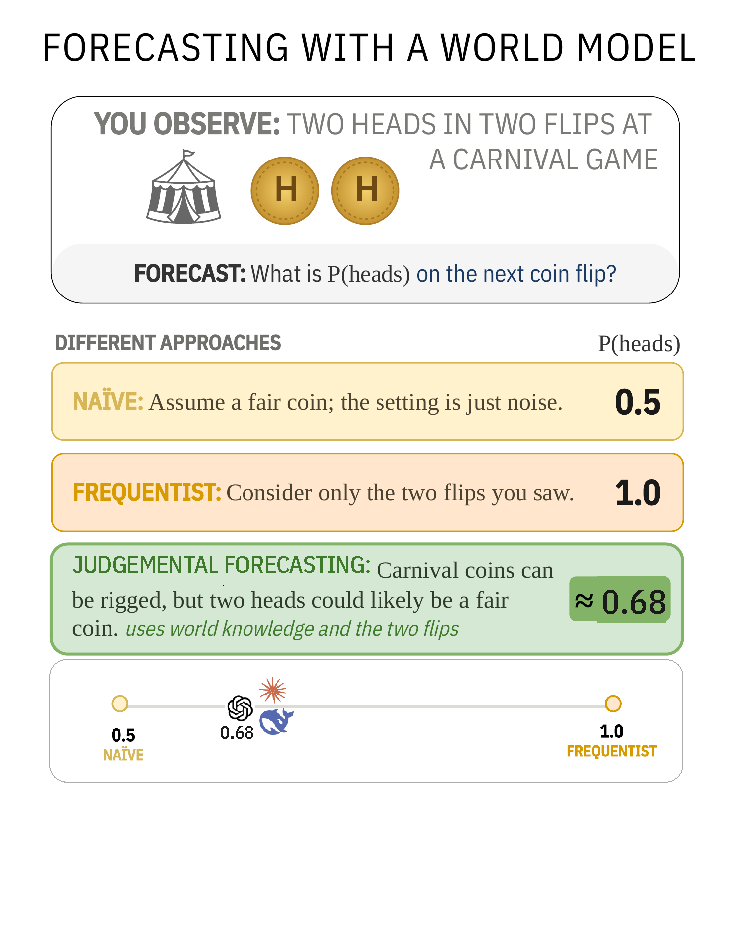
\includegraphics[width=\linewidth,trim=0 72pt 0 0,clip]{figures/teaser_revised.pdf}
\vspace{-0.6cm}
\caption{ \textbf{LM forecasts are not solely na\"\i ve or frequentists.}
\small
After two heads in a carnival coin game, LMs forecast another head more often
when the coin may be rigged. Mean forecasts are $.644$, $.681$, and $.712$ for
GPT-5.4, Claude Opus~4.8, and DeepSeek V4-Pro, respectively, over 8
temperature-$0.7$ calls each (Appendix~\ref{app:carnival-coin-probe}).}
\vspace{-0.5cm}
\label{fig:world-knowledge-evidence}
\end{wrapfigure}

Language models (LMs) achieve forecasting accuracy near a human crowd; ensembles
match it on some question sets \citep{halawi2024approaching,schoenegger2024wisdom}.
Results on Metaculus, Polymarket, and Kalshi
\citep{lu2025evaluating,cao2026auditable,zhang2026prediction} raise the question:
\emph{why are LMs competitive forecasters?} Accuracy alone cannot distinguish a
base rate, retrieved case, market signal, or predictive relationship. These
strategies can agree on familiar questions but diverge when context changes.

Figure~\ref{fig:world-knowledge-evidence} illustrates the distinction. After two
heads, the next-flip probability stays at $0.5$ for a known-fair coin but rises
when the carnival setting makes persistent bias plausible. Context, not changed
observations, selects the past--future relationship. \textbf{Judgmental
forecasting} performs this operation routinely, combining base rates, sparse
observations, qualitative evidence, and domain knowledge to estimate future
events \citep{mellers2014psychological,tetlock2016superforecasting}.


In this paper, we ask whether LM forecasts exhibit behavioral signatures of this process, which we refer to as \emph{inductive reasoning}: the selection of a predictive relationship from context and sparse observations, the revision of that selection as evidence accumulates, and the application of the relationship to a new case \citep{tenenbaum2006theory,tenenbaum2011mind,griffiths2010probabilistic,lake2015human,lake2017building}. We use \emph{world structure} to denote the predictive relationships among variables. Both definitions are behavioral and presume neither an explicit graph nor a particular internal representation.

Pointwise accuracy cannot identify this process, and generated explanations need not reflect it \citep{jacovi2020towards,turpin2023language}. We, therefore, intervene on forecasts and measure the resulting change under contrasts with predicted directions \citep{ribeiro2020beyond,elazar2021measuring}: varying evidence direction while holding topic fixed, reversing a context--regime assignment while holding all numerical inputs fixed, adding observations that conflict with a contextual cue, and preserving the distribution of training answers while breaking their episode-level correspondence.

\subsection{Empirical Progression}
\label{sec:forecasting-as-inductive}

The four experiments form a progression organized by three questions:
\begin{itemize}[nosep,leftmargin=*]
  \item \textbf{Do LMs react selectively to evidence?
  (\hyperref[sec:exp1]{Experiment~1}).}
  Across 30,094 updates on unresolved real questions, nine models move
  $1.9$--$24\times$ farther for directional evidence than for topically matched
  controls, and follow packet sign at $.89$--$.99$, where a market-held-out lexical
  classifier reaches $.69$ and human readers $.76$. Packets withhold their polarity,
  so the sign result is not surface matching, though the arms differ in wording and
  the relationships involved are ones models already hold.
  \item \textbf{Can an LM select a relationship based on context?
  (\hyperref[sec:exp2]{Experiment~2}).}
  A cue selects one of two response regimes: reversing it reverses forecasts,
  and target observations weaken its effect. When arbitrary cue meanings reverse
  across episodes, twelve of fifteen systems recover the new mapping, every hosted
  one among them, and within Qwen3 and Llama only the larger checkpoints do. On
  sealed episodes, linear probes of five open checkpoints decode the cue-selected
  regime exactly where forecasts recover the mapping, and patching that
  representation moves Qwen3-14B's zero-shot forecast.
  \item \textbf{Are finetuned LMs able to transfer contextual relationships?
  (\hyperref[sec:exp3]{Experiments~3} and~\hyperref[sec:exp4]{4}).}
  Under joint domain-and-mechanism shift, Qwen3-8B episode-matched response MAE is
  $.25$ $[.06,.47]$ lower than the population-prior control, with the same direction
  at 4B. On a new 318-market holdout, trained Brier falls from $.1366$ to
  $.1286$ to $.1270$ across Qwen3-4B, 8B, and 14B; the 14B score differs from
  the contemporaneous Polymarket crowd by $+.0004$ $[-.0003,+.0014]$.
\end{itemize}

\section{Related work: why accuracy is not enough}
\label{sec:related-work}

\noindent\textbf{Judgmental forecasting.}
Strong human forecasters combine base rates, decomposition, diverse evidence,
and repeated revision
\citep{tetlock2005expert,mellers2014psychological,tetlock2016superforecasting}.
LM benchmarks increasingly use time-indexed or leakage-controlled questions, and
retrieval or ensembling can bring systems near crowd accuracy
\citep{zou2022forecasting,karger2025forecastbench,halawi2024approaching,schoenegger2024wisdom}.
These results establish what probabilities models can produce. They do not tell
us what would make those probabilities change.

\noindent\textbf{Induction and relational reasoning.}
Transformers can infer functions from examples, and work on analogy and world
models asks whether learned representations capture relations or dynamics
\citep{garg2022what,chan2022data,webb2023emergent,yasunaga2024large,ha2018world,lecun2022path,li2023emergent}.
At the same time, shortcut research shows that surface success can fail under
structural change
\citep{geirhos2020shortcut,mitchell2023ai,vafa2025foundation}. A forecast can
therefore be right for the wrong reason: two models may report the same number
while relying on different populations, evidence, or pathways.

\noindent\textbf{Social agents and conditional validity.}
Generative agents can reproduce plausible individual and collective behavior
\citep{park2023generative,aher2023simulate,argyle2023out}, yet matching a
population average is not the same as preserving the relationships within that
population \citep{bisbee2024synthetic}. For systems intended to inform decisions,
we care about both the \emph{probability reported} and the \emph{relationship
that makes the evidence predictive}. Our experiments therefore move through
increasingly stringent tests: relevance and direction, contextual relationship
selection, revision from local evidence, induction of a novel convention, and
transfer across worlds. Each step rules out a weaker account of the same
forecast without assuming a general internal world model.

\section{Methods}
\label{sec:methods}

We pair controlled simulations with prospective and historical Polymarket questions
\citep{gentzel2019case,polymarket2026docs}. Simulations isolate information sources;
the market studies test evidence use on open questions and accuracy on held-out,
resolved events. Contrasts are paired by question or episode. For trained models,
uncertainty is propagated first across seeds and then across episodes within seed.

The sequence distinguishes four steps: relevance-sensitive updating, contextual
relationship selection, learning the episode-level evidence--outcome mapping, and
transfer to unseen synthetic mechanisms and real-event families.


\subsection{Experiment 1: Evidence-Selective Updating}
\label{sec:methods-exp1}

We sample 100 binary markets in politics, government, elections, economics, technology, and
geopolitics, each open at collection, 14--180 days from resolution, and with at
least \$1,000 in lifetime USD volume. We report three
hosted API systems \citep{openai2026gpt54,anthropic2026claude48,deepseek2026v4}
and six scale-valid Qwen~2.5 or Llama-family open-weight models
\citep{qwen2025qwen25,grattafiori2024llama}; Appendix~\ref{app:record-processing}
retains one mixed-scale deployment for compliance diagnostics.

Agents return an event model and $P(H_1)$ (YES), $P(H_2)$ (NO), with headline
forecast $\hat p=P(H_1)$. With search then disabled, they receive nine generated
packets per market---three pro-$H_1$, three anti-$H_1$, three topical but
orthogonal---giving 30,094 valid updates. The prompt carries one packet field, the
snippet text; every other field is withheld and read only at scoring
(Appendix~\ref{app:exp1-withholding}).

We report three measures. \textbf{Abstention} is the share of orthogonal
updates returning the displayed prior unchanged; \textbf{sensitivity} divides mean
absolute directional by orthogonal movement among updates that moved at all. Both
ask whether a model discriminates probative from topic-matched evidence. \textbf{Evidence--Hypothesis Consistency
(EHC)} is directional correctness for stated $P(H_1)$ among updates of at least 3
points and asks whether the forecast moves the predicted way. Appendix~\ref{app:exp1-alternatives}
gives lexical and human comparisons for packet-direction recovery and alternative
selectivity estimands. Figure color bands use
sensitivity cutpoints $2.5,4,6$ and EHC cutpoints $.90,.95,.98$. Intervals use
20,000 market-clustered resamples retaining all packets and repeated initial runs
(Appendix~\ref{app:exp1-threshold-robustness}). Eight reviewers judged 18
balanced packets against the frozen direction key, matching it on 75.0\%;
Appendix~\ref{app:exp1-limitations} gives the tally, the disclosed
post-inspection exclusion, and item-level judgments.


\begin{figure}[!ht]
\centering
% The exported figure carries ~14.5pt of blank canvas below its last box;
% trim most of it so the caption sits closer than the export padding allows.
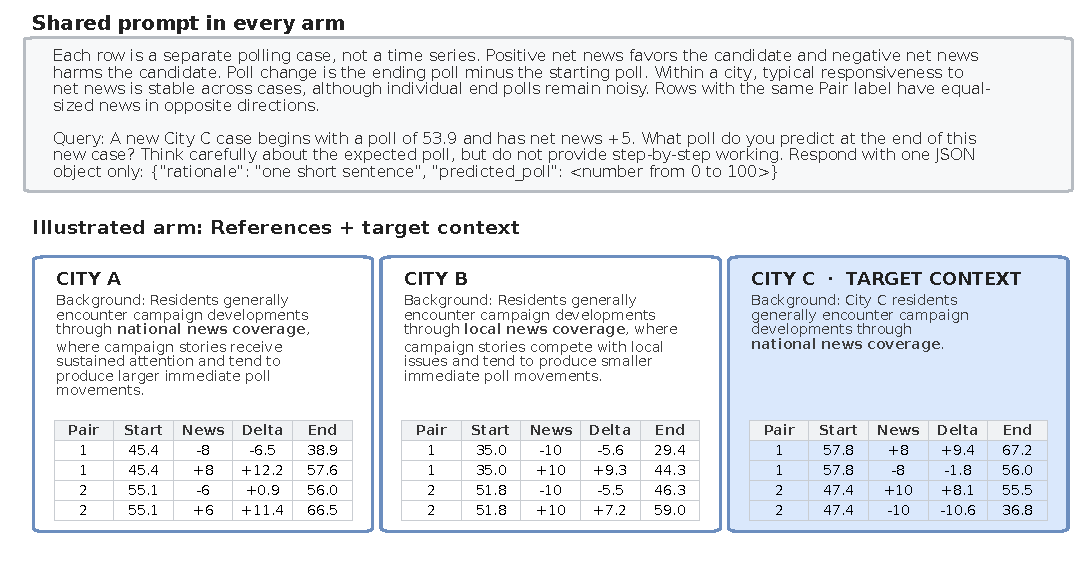
\includegraphics[width=\linewidth,trim=0 10pt 0 0,clip]{figures/exp2_coin_city_prompt_arms.pdf}
\caption{\textbf{Coin City prompt and information arms.} Every arm receives the
instructions and query shown. The illustrated episode ($k=4$) additionally provides
City A/B references and City C's qualitative context. The no-context and
opposite-context arms change only the City C sentence.}
\label{fig:coin-city-prompts}
\end{figure}

\subsection{Experiment 2: Context-Guided Relationship Selection}
\label{sec:methods-stage2}

\label{sec:methods-coin-city}

Each Coin City episode describes three cities with stable but unobserved poll
responses to news. City A and City B provide reference cases; City C provides up to
four observations and a one-sentence description naming a response regime. The
reference descriptions state which regime responds more strongly, but no prompt
states a coefficient.

We generate 250 independent episodes. For city $j$ in episode $i$,
\begin{equation}
  \Delta p_{ij}=g_jx_{ij}+\epsilon_{ij},
  \qquad \epsilon_{ij}\sim\mathcal N(0,5^2),
  \label{eq:coin-city-dgp}
\end{equation}
where $x_{ij}$ is signed net news, and strong and weak cities draw
$g_j\sim\mathcal N(0.90,0.03^2)$ and $g_j\sim\mathcal N(0.25,0.03^2)$. Each
reference city provides four cases in matched equal-and-opposite news pairs. A
query asks for City C's ending poll after news
$x\in\{-10,\ldots,-4,4,\ldots,10\}$, given $k\in\{0,1,2,3,4\}$ City C cases.

Five prompt arms vary the evidence available: target cases alone; reference cases
without City C context; references with the correct City C context; references with
the opposite context label; and an arbitrary-label arm replacing national/local
with \texttt{KIV}/\texttt{ZOR}, whose higher-response mapping changes by episode
and must be recovered from the reference cases. Paired arms share the same episode
and query values; the correct- and opposite-context prompts differ only in City C's
context sentence. Every arm reuses an episode bank under a manifest hashed before model calls
(Figure~\ref{fig:coin-city-prompts}). An open-weight activation audit reuses the
semantic and arbitrary-label arms' correct, absent, and inverted prompts and patches
the label tokens. Appendix~\ref{app:coin-city} gives full design and execution
details.

Claude Opus~4.8, Claude Opus~5, GPT-5.6, DeepSeek-V4-Pro, Kimi K3, and Gemini 3.6
Flash are evaluated on every frozen episode, evidence depth, and four semantic arms:
30,000 attempts in total. The arbitrary-label analysis extends the roster to 15
systems at $k=0$ and evaluates open-weight scale families. Forecast MAE is measured against the noise-free expectation
$p_0+g_Cx$; the forecast-implied response $\hat g=(\hat p-p_0)/x$ is reported as
MAE and as across-episode correlation with $g_C$.

A deterministic analogical benchmark uses the cue to choose City A or B, fits that
reference by through-origin OLS, and refits as City C cases arrive
(Appendix~\ref{app:coin-city-analysis}). Paired intervals use 2,000 episode
bootstrap samples \citep{efron1979bootstrap}.

\subsection{Experiment 3: Controlled Relationship Transfer}
\label{sec:methods-stage3}

\label{sec:methods-exp3-synthetic}

% Compact inline orientation graphic for the Experiment 3 transfer design: a 2x2
% grid crossing generative mechanism (rows) with surface domain (columns).
%
% Row cards carry the mechanism detail: a two-node vs three-node graph with the
% mediator drawn hollow (it is never named to the model) and a persistence loop,
% plus the six-period impulse response on labelled axes. Bar heights are the
% normalised responses to a unit shock under worlds.transition at the midpoint of
% each sampling band (direct: gain .57; mediated: gain .57, rho .61, phi .30,
% lambda .81), i.e. A = (1, 0, 0, 0, 0, 0) and B = (.81, .74, .52, .34, .21, .13).
%
% Geometry note: cards have fixed dimensions and every label is a single line
% with no text width, so nothing can rewrap into a neighbour.
\begin{wrapfigure}{r}{0.40\textwidth}
\vspace{-0.7em}
\centering
\definecolor{miniCityFill}{HTML}{E8F2FB}
\definecolor{miniCityEdge}{HTML}{4F7EA8}
\definecolor{miniHarborEdge}{HTML}{3F8E82}
\definecolor{miniTestFill}{HTML}{E7F4EA}
\definecolor{miniTestEdge}{HTML}{6FA97F}
\definecolor{miniTestChip}{HTML}{5E9470}
% Coin discs reuse Figure 1's yellow pair exactly -- the fill and stroke of its
% NAIVE box -- rather than the saturated gold used before. Figure 1's other warm
% pair (#FFE6CC on #D79B00, its FREQUENTIST box) is the orange one and is not
% used here. The glyph inside each disc still carries its domain colour.
\definecolor{miniCoinFill}{HTML}{FFF2CC}
\definecolor{miniCoinRim}{HTML}{D6B656}
\definecolor{miniMute}{HTML}{8A93A3}
\definecolor{miniInk}{HTML}{3F4550}
\definecolor{miniBar}{HTML}{7C93AD}
% Coin City: a skyline stamped into a coin.
\newcommand{\coincity}[2]{%
  \begin{scope}[shift={(#1,#2)},scale=0.70]
    \fill[miniCoinFill] (0,0) circle (.37);
    \draw[miniCoinRim,line width=.75pt] (0,0) circle (.37);
    \fill[miniCityEdge] (-.23,-.18) rectangle (-.10,.04);
    \fill[miniCityEdge] (-.07,-.18) rectangle (.07,.16);
    \fill[miniCityEdge] (.10,-.18) rectangle (.24,.09);
    \draw[miniCityEdge,line width=.65pt] (-.27,-.19)--(.27,-.19);
  \end{scope}}
% Coin Harbor: a small vessel and waves stamped into a coin.
\newcommand{\coinharbor}[2]{%
  \begin{scope}[shift={(#1,#2)},scale=0.70]
    \fill[miniCoinFill] (0,0) circle (.37);
    \draw[miniCoinRim,line width=.75pt] (0,0) circle (.37);
    \fill[miniHarborEdge] (-.24,-.05)--(.24,-.05)--(.15,-.18)--(-.15,-.18)--cycle;
    \draw[miniHarborEdge,line width=.7pt]
      (-.01,-.05)--(-.01,.15)--(.15,.02)--(-.01,.02);
    \draw[miniHarborEdge,line width=.55pt]
      (-.26,-.24)..controls(-.18,-.19)and(-.10,-.29)..(-.02,-.24)
      ..controls(.06,-.19)and(.14,-.29)..(.26,-.24);
  \end{scope}}
% Impulse response on labelled axes: response (Delta y) against period (t).
\newcommand{\impulse}[3]{% #1 = axis corner x, #2 = baseline y, #3 = bar heights
  \draw[-{Stealth[length=2.6pt,width=2.2pt]},draw=miniInk!65,line width=.5pt]
    (#1,#2) -- (#1,#2+0.40);
  \draw[-{Stealth[length=2.6pt,width=2.2pt]},draw=miniInk!65,line width=.5pt]
    (#1,#2) -- (#1+0.72,#2);
  \node[anchor=south,font=\sffamily\scriptsize,text=miniInk,inner sep=1pt]
    at (#1,#2+0.40) {$\Delta y$};
  \node[anchor=west,font=\sffamily\scriptsize,text=miniInk,inner sep=1.5pt]
    at (#1+0.72,#2) {$t$};
  \foreach \i/\h in {#3}{%
    \fill[miniBar] (#1+0.055+\i*0.105,#2) rectangle (#1+0.055+\i*0.105+0.070,#2+\h);}}
\resizebox{\linewidth}{!}{%
\begin{tikzpicture}[
  x=1cm, y=1cm,
  cell/.style={rounded corners=3pt, minimum width=1.95cm, minimum height=1.25cm,
    line width=.6pt, inner sep=0pt},
  traincell/.style={cell, draw=miniCityEdge, fill=miniCityFill},
  heldcell/.style={cell, draw=miniTestEdge, fill=miniTestFill,
    dash pattern=on 1.9pt off 1.5pt},
  rowcard/.style={rounded corners=3pt, minimum width=2.60cm,
    minimum height=1.25cm, inner sep=0pt, draw=miniMute!30, fill=black!3,
    line width=.5pt},
  dname/.style={anchor=south, font=\sffamily\bfseries\scriptsize},
  rname/.style={anchor=center, font=\sffamily\scriptsize, text=miniInk},
  note/.style={anchor=center, font=\sffamily\scriptsize, text=miniInk},
  gnode/.style={circle, draw=miniInk!75, fill=white, line width=.5pt,
    inner sep=0pt, minimum size=0.26cm, font=\sffamily\tiny, text=miniInk},
  hidden/.style={gnode, draw=miniMute, fill=miniMute!14,
    dash pattern=on 1.1pt off .9pt},
  garrow/.style={-{Stealth[length=2.4pt,width=2pt]}, draw=miniInk!70,
    line width=.45pt, shorten >=.4pt, shorten <=.4pt},
  chip/.style={anchor=center, rounded corners=1.6pt, draw=none, text=white,
    inner xsep=3pt, inner ysep=1.1pt, font=\sffamily\bfseries\tiny},
]
% ---- domain marks and names ----------------------------------------------
\coincity{0.975}{2.56}
\coinharbor{3.075}{2.56}
\node[dname, text=miniCityEdge]   at (0.975,1.80) {COIN CITY};
\node[dname, text=miniHarborEdge] at (3.075,1.80) {COIN HARBOR};

% ---- Structure A: direct, one period -------------------------------------
\node[rowcard] at (-1.50,1.00) {};
\node[rname] at (-1.50,1.45) {\textbf{Structure A} direct};
\node[gnode] (ax) at (-2.51,0.82) {$x$};
\node[gnode] (ay) at (-2.07,0.82) {$y$};
\draw[garrow] (ax) -- (ay);
\impulse{-1.22}{0.62}{0/0.360, 1/0.000, 2/0.000, 3/0.000, 4/0.000, 5/0.000}

% ---- Structure B: mediated, persistent -----------------------------------
\node[rowcard] at (-1.50,-0.42) {};
\node[rname] at (-1.50,0.03) {\textbf{Structure B} mediated};
\node[gnode]  (bx) at (-2.51,-0.60) {$x$};
\node[hidden] (bm) at (-2.07,-0.60) {$m$};
\node[gnode]  (by) at (-1.63,-0.60) {$y$};
\draw[garrow] (bx) -- (bm);
\draw[garrow] (bm) -- (by);
\draw[garrow] (bm) to[out=118,in=62,looseness=4.5] (bm);
\impulse{-1.22}{-0.80}{0/0.292, 1/0.265, 2/0.188, 3/0.123, 4/0.077, 5/0.048}

% ---- the four evaluation cells -------------------------------------------
\node[traincell] at (0.975,1.00) {};
\node[heldcell]  at (3.075,1.00) {};
\node[heldcell]  at (0.975,-0.42) {};
\node[heldcell]  at (3.075,-0.42) {};

\node[chip, fill=miniCityEdge] at (0.975,1.26) {TRAINED};
\node[chip, fill=miniTestChip] at (3.075,1.26) {TEST};
\node[chip, fill=miniTestChip] at (0.975,-0.16) {TEST};
\node[chip, fill=miniTestChip] at (3.075,-0.16) {TEST};

\node[note] at (0.975,0.80) {in-distribution};
\node[note] at (3.075,0.80) {domain shift};
\node[note] at (0.975,-0.62) {structure shift};
\node[note] at (3.075,-0.62) {joint shift};
\end{tikzpicture}%
}
\vspace{-0.3em}
\caption{\footnotesize\textbf{Transfer grid.} Training uses the shaded cell only; all
four are evaluated. Bars are each mechanism's response $\Delta y$ over the
periods $t$ following one shock: A returns to baseline at once, B builds through
the unobserved mediator $m$ and persists.}
\label{fig:exp3-transfer-grid}
\vspace{-0.5em}
\end{wrapfigure}

Training uses the direct, one-period relationship in
Equation~\ref{eq:coin-city-dgp}. Each prompt shows two complete 14-case references,
a target with $k$ observed cases, and a ten-outcome query. The episode-matched and
population-prior arms use byte-identical prompts and the same multiset of answer
keys. Matched training pairs episode $i$ with its own key $\mathbf y^\star_i$;
the control uses a fixed within-$k$ derangement $\mathbf y^\star_{\pi_k(i)}$.
This preserves the answer distribution while breaking the prompt--target link,
making the contrast a training analogue of Experiment~2: only the matched arm
rewards recovering the episode-specific evidence--outcome mapping. Neither arm
supplies graph labels. A structureless diagnostic scrambles the
displayed drivers and rewards a flat response; the untrained base receives the
same evaluation prompts without training.
Table~\ref{tab:exp3-training-policies}
in Appendix~\ref{app:exp3-coin-structural} shows all four conditions on one episode.


Policies train only on Coin City under Structure~A, the direct mechanism
$x_t\to y_{t+1}$. Figure~\ref{fig:exp3-transfer-grid} crosses this trained cell
with a new surface domain (Coin Harbor), the mediated Structure~B
($x_t\to m_{t+1}\to y_{t+1}$), and both shifts together.

Evaluation crosses domain, mechanism, pathway hint, and
$k\in\{0,2,4,8\}$, yielding $1{,}440$ paired prompts; each training run contains
4,800 Coin City/Structure~A prompts. The primary estimand is population-prior
minus episode-matched response MAE under joint shift and the correct hint. The
joint cell asks whether learning to bind each prompt to its own response pattern
transfers beyond the domain and mechanism on which that binding was rewarded. We use
three Qwen3-8B seeds per arm at round 300 and average five stochastic draws within
task before a paired seed-first bootstrap. The Qwen3-4B scale replication,
structureless control, Llama-8B comparator, prompts, and parameters appear in
Appendix~\ref{app:exp3-coin-structural}.

\begin{figure}[b]
\centering
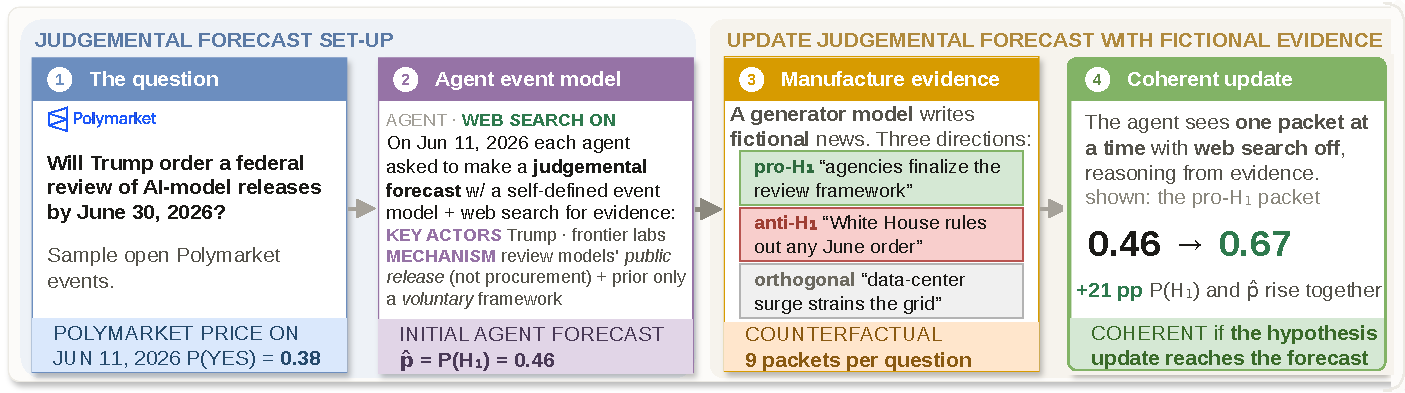
\includegraphics[width=\linewidth]{figures/exp1_protocol_four_panels.pdf}
\caption{\textbf{Prospective evidence-intervention protocol.} An agent forecasts an
unresolved question, then receives one generated evidence packet with search off.
The packet's intended direction is never shown to the agent; it is read only when
the update is scored.
Directional correctness asks whether the update follows a pro- or anti-$H_1$
packet. Selectivity compares movement under directional and orthogonal packets.
The output contract requires $\hat p=P(H_1)$, so agreement between those fields is
partly schema compliance.}
\label{fig:exp1-pipeline}
\end{figure}

\subsection{Experiment 4: Historical-Market Training and Sealed Evaluation}
\label{sec:methods-exp4-polymarket}

Experiment~4 moves from identified synthetic relationships to real questions,
where the relevant structure is unobserved. It tests whether outcome training
generalizes to unseen event families, not which relationship the model inferred.
Resolved political, governmental, macroeconomic, and geopolitical markets are cut
off 30 days before their earliest archived terminal timestamp. Prompts retain only
the question, rules, cutoff, and genuine pre-cutoff prices. Outcomes and post-cutoff
fields are withheld. Calendar splits contain 1,736 training, 512 development, and
1,024 test markets, with no event or normalized question family shared across
splits.

We train Qwen3 and Llama checkpoints \citep{qwen2025qwen3,grattafiori2024llama} with
rank-32 LoRA \citep{hu2022lora} and Dr.~GRPO
\citep{liu2025understanding} for 300 rollout-and-update rounds (4,800 prompt
presentations) at each of three seeds. Reward is the proper score
$1-(\hat p-y)^2$ \citep{brier1950verification}; training alone supplies
gradients. Development selects no endpoint, and test data are absent from
training.

The scale comparison evaluates three-seed Qwen3 checkpoints at 1.7B, 4B, 8B, 14B, and
32B parameters and Llama checkpoints at 3B and 8B on a 318-market holdout disjoint
from all training, development, and test families. Every base and trained endpoint is
scored from five non-thinking stochastic draws. Brier intervals resample connected
event/template families \citep{brier1950verification,good1952rational}. A Qwen3-4B
evidence-updating evaluation also applies the Experiment~1 packets to the base and
final adapters. Appendix~\ref{app:exp3b-protocol} gives the censoring, checksums,
optimization, held-out evaluation, scale comparison, and revision-analysis details.

\section{Results}
\label{sec:results}

Results follow an inductive-forecasting progression. Experiment~1 tests whether
updates distinguish probative from topic-matched evidence. Experiment~2 tests
whether context selects an episode-local relationship and observations revise it.
Experiment~3 asks whether training that episode-level mapping transfers across a
controlled domain-and-mechanism shift. Experiment~4 asks whether outcome training
generalizes to unseen real-event families, where accuracy can establish transfer
but cannot identify the relationship used.

\begin{figure}[!ht]
\centering
\begin{subfigure}[c]{0.525\textwidth}
\centering
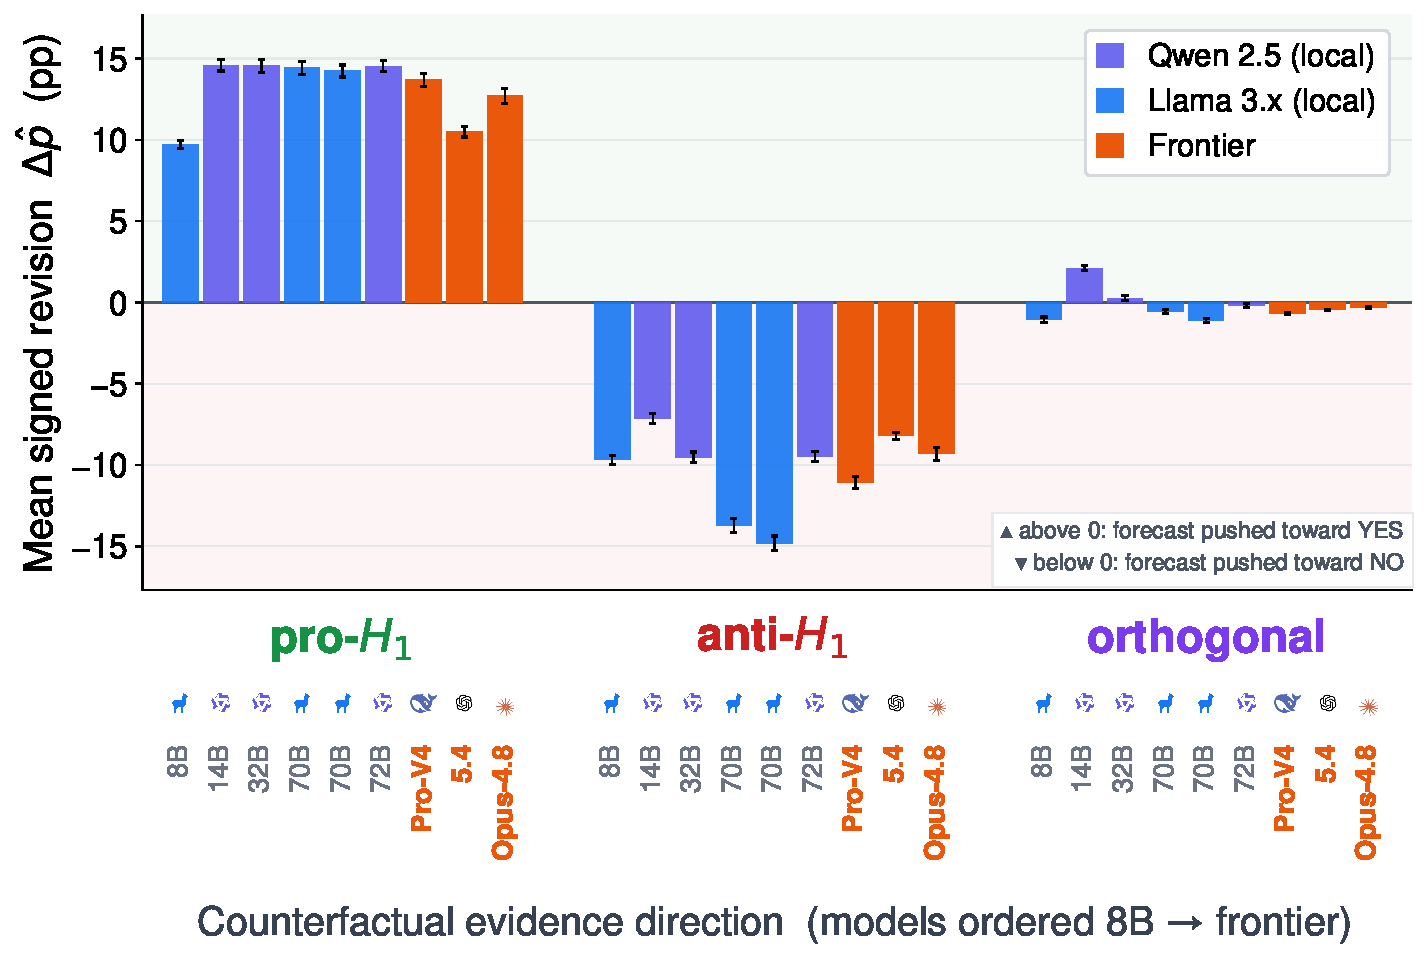
\includegraphics[width=\linewidth]{figures/exp1_direction_selective_updating.pdf}
\caption{}
\label{fig:exp1-bars}
\end{subfigure}\hspace{0.01\textwidth}
\begin{subfigure}[c]{0.455\textwidth}
\centering
\footnotesize
\setlength{\tabcolsep}{3pt}
\begin{tabular*}{\linewidth}{@{}l@{\extracolsep{\fill}}rccc@{}}
\toprule
\textbf{Model} & \textbf{Size} & \textbf{Abst.} & \textbf{Sens.}$\uparrow$ & \textbf{EHC$_{\geq3}$}$\uparrow$ \\
\midrule
\multicolumn{5}{@{}l}{\emph{Hosted API (parameters undisclosed)}}\\
\micon{claude.png}~Opus~4.8 & --- & 71.4\% & \cellcolor{heatgreen}$7.0\times$ & \cellcolor{heatgreen}.990 \\
\micon{openai.png}~GPT-5.4 & --- & 8.4\% & \cellcolor{heatgreen}$7.5\times$ & \cellcolor{heatgreen}.987 \\
\micon{deepseek.png}~V4-Pro & --- & 44.4\% & \cellcolor{heatyellow}$4.9\times$ & \cellcolor{heatyellow}.977 \\
\midrule
\multicolumn{5}{@{}l}{\emph{Open-weight, descending parameters} $\downarrow$}\\
\micon{qwen.pdf}~2.5-72B & 72B & 24.2\% & \cellcolor{heatorange}$3.2\times$ & \cellcolor{heatyellow}.963 \\
\micon{llamma.pdf}~3.3-70B & 70B & 10.7\% & \cellcolor{heatyellow}$5.7\times$ & \cellcolor{heatyellow}.965 \\
\micon{llamma.pdf}~3.1-70B & 70B & 2.5\% & \cellcolor{heatyellow}$4.5\times$ & \cellcolor{heatyellow}.961 \\
\micon{qwen.pdf}~2.5-32B & 32B & 11.1\% & \cellcolor{heatorange}$2.8\times$ & \cellcolor{heatyellow}.964 \\
\micon{qwen.pdf}~2.5-14B & 14B & 26.1\% & \cellcolor{heatred}$2.2\times$ & \cellcolor{heatorange}.943 \\
\micon{llamma.pdf}~3.1-8B & 8B & 1.1\% & \cellcolor{heatred}$1.9\times$ & \cellcolor{heatred}.887 \\
\bottomrule
\end{tabular*}
\caption{}
\label{fig:exp1-table}
\label{tab:consistency}
\end{subfigure}
\caption{\textbf{Direction-selective updating across nine models and 30,094 valid update
records.} \textbf{(a)} Mean signed forecast revision by counterfactual direction;
error bars are 95\% market-clustered bootstrap intervals. The orthogonal arm
carries no intended sign, so its signed mean is near zero by construction; its
absolute revisions are $0.5$--$5.9$~pp. \textbf{(b)} Hosted systems first,
open-weight rows in descending parameter count; measures and color bands are
defined in Methods, and abstention is uncolored because a high rate is not
unambiguously better. Appendix Table~\ref{tab:exp1-abstention} gives the product
of the two selectivity measures, and
Appendix~\ref{app:exp1-threshold-robustness} the output-field compliance and
threshold sweep.}
\label{fig:exp1-updating}
\end{figure}

\subsection{Experiment 1: Evidence-Selective Forecast Updating}
\label{sec:exp1}

Experiment~1 asks whether forecasts respond to probative evidence more than to
topic-matched controls. The agent sees only its own prior forecast and the
snippet: no packet names $H_1$, $H_2$, or the market's resolution, and 2.4\% use
any likelihood wording at all (Appendix~\ref{app:exp1-withholding}). The direction
key is therefore never supplied, although the snippet's words can carry partial
directional signal.

\textbf{Discrimination.} Selective updating has two separable components, and the
table reports them side by side. The first is declining to revise at all: every
deployment holds the prior on $1.1$--$71.4\%$ of topic-matched controls but on
only $0.0$--$1.4\%$ of directional packets. The second is how far it moves when it
does move, which is $1.9$--$7.5\times$ farther on directional packets, every
market-clustered 95\% interval excluding one. A ratio can be inflated by a small
denominator, so two checks avoid dividing: every model moves further on
directional packets in every market it covers, and the within-market probability
that it does so for a random packet pair runs from $.791$ to $.994$. Hosted
systems lead on both components on average, but neither separates the two classes
(Appendix~\ref{app:exp1-alternatives}).

\textbf{Directional correctness.} Across 30,094 valid updates, EHC runs from .887
to .990. All three hosted agents exceed .97; without the three-point movement
threshold, their correctness remains 97.3--98.4\%. A bag-of-words classifier trained on the packet
texts, markets held out, recovers the sign at $.688$, and adding the market
question does not help. Eight human reviewers match the frozen direction on
75.0\% of judgments in a smaller, categorical materials check (pairwise
$\kappa=.47$; Appendix~\ref{app:exp1-human-review}). The tasks are not a
human--model ranking. They show that wording carries partial signal, but this
shallow classifier falls well short of the agents' $.89$--$.99$ directional
accuracy. This within-directional-arm comparison does not depend on the
orthogonal arm's different wording.

Two caveats qualify the selectivity result. Wording differs across arms, so models
may use arm-correlated cues rather than derive relevance, although stated relevance
predicts their updates (Appendix~\ref{app:exp1-alternatives}). The tested
relationships may also be familiar; Experiment~2 requires inferring a novel one.
Full protocol, robustness, and materials details appear in
Appendix~\ref{app:exp1}.

\subsection{Experiment 2: Context-Conditioned Relationship Selection}
\label{sec:exp2}

Experiment~2 asks which numerical relationship a model applies to a new target.
Two reference cities demonstrate a strong and a weak response regime, a
one-sentence cue assigns target City C to one of them, and City C's own cases
accumulate from $k=0$ to $k=4$. Arms are matched on every displayed number, so a
contrast isolates the cue. Because the reference sentences state which regime
responds more strongly, the semantic arms measure how a stated assignment becomes
a number; the induction claim rests on an arbitrary-label arm whose
\texttt{KIV}/\texttt{ZOR} mapping reverses across episodes.
Appendix~\ref{app:coin-city} gives prompts, results and analysis details.

\begin{figure}[!ht]
\centering
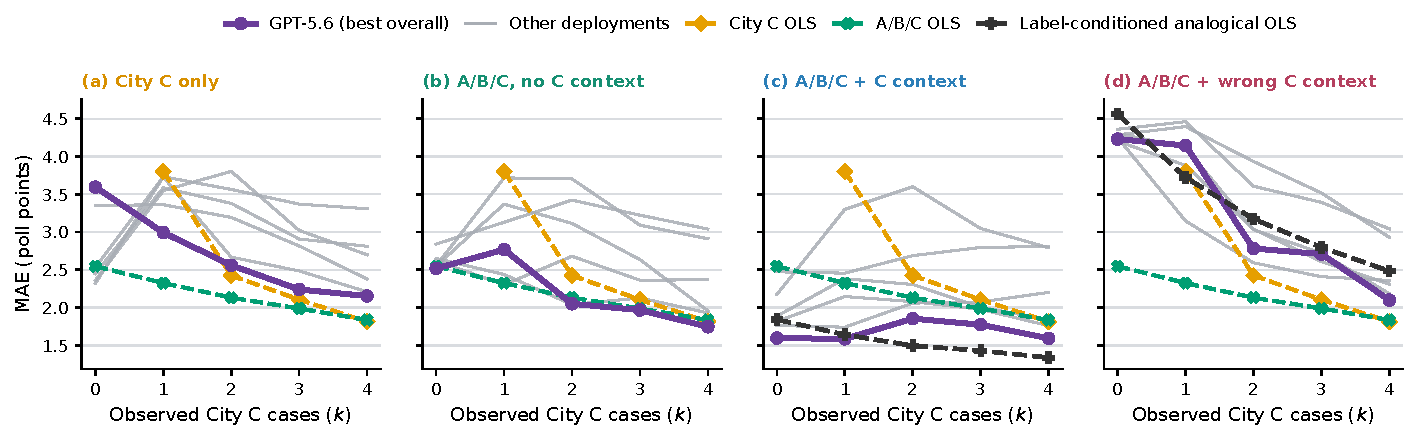
\includegraphics[width=\linewidth]{figures/exp2_coin_city_results.pdf}
\vspace{3pt}
\begin{minipage}{\linewidth}
\centering
\footnotesize
\setlength{\tabcolsep}{4pt}
\resizebox{\linewidth}{!}{%
\begin{tabular}{l r rrrr rr}
\toprule
& & \multicolumn{4}{c}{Forecast MAE [95\% CI]} & \multicolumn{2}{c}{$\rho(\hat g,g_C)$} \\
\cmidrule(lr){3-6}\cmidrule(lr){7-8}
Model & Paired $n$ & Target only & No C context & $+$ C context &
$+$ wrong C context & No context & $+$ context \\
\midrule
\micon{claude.png}~Opus~4.8 & 250 & 2.32 [2.20,\,2.46] & 2.65 [2.41,\,2.89] & \textbf{1.82} [1.64,\,2.02] & 4.20 [3.87,\,4.54] & $-.06$ & \textbf{.70} \\
\micon{claude.png}~Opus~5 & 250 & 2.36 [2.12,\,2.59] & 2.62 [2.38,\,2.84] & \textbf{1.76} [1.57,\,1.99] & 4.25 [3.92,\,4.57] & $-.01$ & \textbf{.62} \\
\micon{openai.png}~GPT-5.6 & 250 & 3.60 [3.28,\,3.94] & 2.52 [2.33,\,2.75] & \textbf{1.60} [1.42,\,1.77] & 4.23 [3.90,\,4.55] & $-.04$ & \textbf{.68} \\
\micon{deepseek.png}~V4-Pro & 250 & \textbf{2.45} [2.27,\,2.61] & 2.84 [2.55,\,3.15] & 2.47 [2.19,\,2.77] & 4.36 [4.01,\,4.74] & $-.03$ & \textbf{.52} \\
\micon{kimi.png}~K3 & 250 & 3.35 [3.04,\,3.67] & 2.55 [2.32,\,2.78] & \textbf{1.89} [1.66,\,2.13] & 4.31 [3.98,\,4.62] & $-.02$ & \textbf{.59} \\
\micon{gemini.png}~3.6 Flash & 250 & 2.53 [2.35,\,2.73] & 2.55 [2.31,\,2.80] & \textbf{2.17} [1.89,\,2.48] & 4.29 [3.94,\,4.66] & $.08$ & \textbf{.56} \\
\bottomrule
\end{tabular}
}
\end{minipage}
\caption{\textbf{Context improves zero-shot forecasts and response-regime assignment
across six deployments.} The plots show forecast MAE as City C observations
accumulate. Panels successively add references, the correct target context, and
a misleading context naming the opposite regime. Gray lines are deployments,
purple is the best overall deployment, and dashed curves are context-blind OLS
benchmarks. The table gives per-model MAE and latent-slope correlation at $k=0$,
with 95\% bootstrap intervals over 2,000 episode resamples. Paired contrasts are
in Appendix~\ref{app:coin-city-results}.}
\label{fig:coin-city-results}
\end{figure}

\textbf{Selection and revision.} The cue lowers zero-shot error for every
deployment, by $0.37$ to $0.92$ poll points with all six paired intervals
excluding zero, and every deployment matches or beats a context-blind OLS
benchmark fitted on all displayed rows
(Appendix Table~\ref{tab:coin-city-vs-ols}). Naming the opposite regime reverses
the assignment rather than degrading it. Both effects are transient: by $k=4$ the
cue advantage narrows to $0.12$--$0.23$ points and the wrong-label penalty to
$-0.01$--$+0.38$, so target observations displace the cue once they disagree.

\textbf{The cue selects a displayed reference, not a prior on its words.} Since
those sentences name the direction, the numbers above could come from a prior
about news coverage alone. Partialling out the regime separates the accounts,
because a fit to four noisy reference cases carries sampling error no
cue-determined prior can reproduce. All four arms then behave as reference
selection predicts at $k=0$: with no reference cases neither loads, with no cue
both load equally, the correct cue concentrates loading on the named reference
($.51$--$.86$) and strips it from the other ($.04$--$.10$), and inversion moves it
wholesale onto the reference the false cue names ($.61$--$.90$). It also explains
why implied-slope correlations plateau near $.66$ rather than $.996$: transferring
a noisy estimate is capped at that estimate's own correlation with the truth
(Appendix~\ref{app:coin-city-reference-selection}).

\textbf{Induction of a novel mapping.} This mapping must be inferred from each
episode's own examples. Twelve of fifteen systems recover it at $k=0$, all five
hosted ones among them, and within both Qwen3 and Llama only the larger
checkpoints do---a transition that differs by family rather than tracking
parameter count. Hidden states carry the mapping weakly and only after
computation: semantic-arm probes reach AUC $1.000$ but read the first transformer
block, where input embeddings alone already reach $1.000$. Under arbitrary labels
that control falls to $.555$ while mid-network AUC is $.678$ for Qwen3-14B and
$.778$ for Qwen2.5-32B, and Llama~3.1-8B---whose forecasts do not recover the
mapping---is null throughout. Patching those states at the two label tokens shifts
Qwen3-14B's forecast by $.333$ at $k=0$ ($p<.0001$) and does nothing at $k=4$
(Appendix~\ref{app:coin-city-mechanistic-probe}).

Context therefore selects which demonstrated relationship a model applies, that
selection reaches a particular displayed reference rather than a remembered
association, and target evidence overrides it. Three things bound the reading. The
cue is binary and the regimes far apart, so selection here is a two-way choice
rather than a graded one. The exact within-regime coefficient is never recovered,
failing in every model--$k$ cell. And the mechanistic evidence covers three open
checkpoints with the causal test on one; the hosted deployments are behavioral
throughout. Experiment~3 tests transfer after episode-matched training.

\subsection{Experiment 3: What Training Transfers, and What It Does Not}
\label{sec:exp3}

% Generated by exp3_training_transfer/render_exp3_paper_macros.py
% Do not edit. Every Experiment 3 number in the prose comes from here.
\providecommand{\eEightBaseParse}{99.83}
\providecommand{\eEightDomainBaseGainCi}{[5.266,5.454]}
\providecommand{\eEightDomainBaseGainParsedCi}{[5.266,5.454]}
\providecommand{\eEightDomainBaseGainParsed}{5.360}
\providecommand{\eEightDomainBaseGain}{5.360}
\providecommand{\eEightDomainBase}{7.30}
\providecommand{\eEightDomainCi}{[-.026,.269]}
\providecommand{\eEightDomainEst}{.110}
\providecommand{\eEightDomainMatched}{1.89}
\providecommand{\eEightDomainPrior}{2.00}
\providecommand{\eEightDomainSignP}{.1445}
\providecommand{\eEightDomainSign}{6/8}
\providecommand{\eEightDomainTci}{[-.072,.292]}
\providecommand{\eEightDomainWild}{.1772}
\providecommand{\eEightG}{8}
\providecommand{\eEightIdBaseGainCi}{[3.437,3.481]}
\providecommand{\eEightIdBaseGainParsedCi}{[3.119,3.163]}
\providecommand{\eEightIdBaseGainParsed}{3.141}
\providecommand{\eEightIdBaseGain}{3.459}
\providecommand{\eEightIdBase}{3.96}
\providecommand{\eEightIdCi}{[.018,.112]}
\providecommand{\eEightIdEst}{.060}
\providecommand{\eEightIdMatched}{.47}
\providecommand{\eEightIdPrior}{.53}
\providecommand{\eEightIdSignP}{.0039}
\providecommand{\eEightIdSign}{8/8}
\providecommand{\eEightIdTci}{[.005,.115]}
\providecommand{\eEightIdWild}{.0089}
\providecommand{\eEightJointBaseGainCi}{[1.063,1.196]}
\providecommand{\eEightJointBaseGainParsedCi}{[.611,.744]}
\providecommand{\eEightJointBaseGainParsed}{.677}
\providecommand{\eEightJointBaseGain}{1.129}
\providecommand{\eEightJointBase}{5.72}
\providecommand{\eEightJointCi}{[-.002,.265]}
\providecommand{\eEightJointEst}{.126}
\providecommand{\eEightJointMatched}{4.53}
\providecommand{\eEightJointPrior}{4.65}
\providecommand{\eEightJointSignP}{.1445}
\providecommand{\eEightJointSign}{6/8}
\providecommand{\eEightJointTci}{[-.035,.287]}
\providecommand{\eEightJointWild}{.0906}
\providecommand{\eEightStructureBaseGainCi}{[-.051,-.023]}
\providecommand{\eEightStructureBaseGainParsedCi}{[-.051,-.023]}
\providecommand{\eEightStructureBaseGainParsed}{-.037}
\providecommand{\eEightStructureBaseGain}{-.037}
\providecommand{\eEightStructureBase}{2.30}
\providecommand{\eEightStructureCi}{[-.056,.040]}
\providecommand{\eEightStructureEst}{-.003}
\providecommand{\eEightStructureMatched}{2.34}
\providecommand{\eEightStructurePrior}{2.34}
\providecommand{\eEightStructureSignP}{.1445}
\providecommand{\eEightStructureSign}{6/8}
\providecommand{\eEightStructureTci}{[-.057,.051]}
\providecommand{\eEightStructureWild}{.9177}
\providecommand{\eFourbBaseParse}{99.97}
\providecommand{\eFourbDomainBaseGainCi}{[6.581,6.802]}
\providecommand{\eFourbDomainBaseGainParsedCi}{[6.581,6.802]}
\providecommand{\eFourbDomainBaseGainParsed}{6.692}
\providecommand{\eFourbDomainBaseGain}{6.692}
\providecommand{\eFourbDomainBase}{8.53}
\providecommand{\eFourbDomainCi}{[-.091,.255]}
\providecommand{\eFourbDomainEst}{.087}
\providecommand{\eFourbDomainMatched}{1.80}
\providecommand{\eFourbDomainPrior}{1.88}
\providecommand{\eFourbDomainSignP}{.3633}
\providecommand{\eFourbDomainSign}{5/8}
\providecommand{\eFourbDomainTci}{[-.130,.303]}
\providecommand{\eFourbDomainWild}{.3569}
\providecommand{\eFourbG}{8}
\providecommand{\eFourbIdBaseGainCi}{[3.075,3.166]}
\providecommand{\eFourbIdBaseGainParsedCi}{[3.075,3.166]}
\providecommand{\eFourbIdBaseGainParsed}{3.121}
\providecommand{\eFourbIdBaseGain}{3.121}
\providecommand{\eFourbIdBase}{3.82}
\providecommand{\eFourbIdCi}{[-.056,.194]}
\providecommand{\eFourbIdEst}{.067}
\providecommand{\eFourbIdMatched}{.67}
\providecommand{\eFourbIdPrior}{.74}
\providecommand{\eFourbIdSignP}{.6367}
\providecommand{\eFourbIdSign}{4/8}
\providecommand{\eFourbIdTci}{[-.091,.225]}
\providecommand{\eFourbIdWild}{.3444}
\providecommand{\eFourbJointBaseGainCi}{[1.362,1.551]}
\providecommand{\eFourbJointBaseGainParsedCi}{[1.362,1.551]}
\providecommand{\eFourbJointBaseGainParsed}{1.457}
\providecommand{\eFourbJointBaseGain}{1.457}
\providecommand{\eFourbJointBase}{6.15}
\providecommand{\eFourbJointCi}{[-.032,.298]}
\providecommand{\eFourbJointEst}{.136}
\providecommand{\eFourbJointMatched}{4.63}
\providecommand{\eFourbJointPrior}{4.76}
\providecommand{\eFourbJointSignP}{.1445}
\providecommand{\eFourbJointSign}{6/8}
\providecommand{\eFourbJointTci}{[-.072,.344]}
\providecommand{\eFourbJointWild}{.1583}
\providecommand{\eFourbStructureBaseGainCi}{[.153,.275]}
\providecommand{\eFourbStructureBaseGainParsedCi}{[.153,.275]}
\providecommand{\eFourbStructureBaseGainParsed}{.214}
\providecommand{\eFourbStructureBaseGain}{.214}
\providecommand{\eFourbStructureBase}{2.66}
\providecommand{\eFourbStructureCi}{[-.075,.179]}
\providecommand{\eFourbStructureEst}{.052}
\providecommand{\eFourbStructureMatched}{2.43}
\providecommand{\eFourbStructurePrior}{2.48}
\providecommand{\eFourbStructureSignP}{.3633}
\providecommand{\eFourbStructureSign}{5/8}
\providecommand{\eFourbStructureTci}{[-.110,.214]}
\providecommand{\eFourbStructureWild}{.4623}
\providecommand{\eMechDiscCi}{[.278,.404]}
\providecommand{\eMechDiscEst}{.337}
\providecommand{\eMechDiscSd}{.073}
\providecommand{\eMechDiscSignP}{.0312}
\providecommand{\eMechDiscSign}{5/5}
\providecommand{\eMechDiscTci}{[.247,.428]}
\providecommand{\eMechDiscWild}{.0130}
\providecommand{\eMechG}{5}
\providecommand{\eMechUndiscCi}{[.328,.387]}
\providecommand{\eMechUndiscEst}{.357}
\providecommand{\eMechUndiscSd}{.033}
\providecommand{\eMechUndiscSignP}{.0312}
\providecommand{\eMechUndiscSign}{5/5}
\providecommand{\eMechUndiscTci}{[.316,.399]}
\providecommand{\eMechUndiscWild}{.0021}
\providecommand{\ePubEightDomainCi}{[.026,.545]}
\providecommand{\ePubEightDomainEst}{.241}
\providecommand{\ePubEightIdCi}{[.002,.187]}
\providecommand{\ePubEightIdEst}{.081}
\providecommand{\ePubEightJointCi}{[.058,.470]}
\providecommand{\ePubEightJointEst}{.251}
\providecommand{\ePubEightStructureCi}{[-.011,.071]}
\providecommand{\ePubEightStructureEst}{.029}
\providecommand{\ePubFourbDomainCi}{[.039,.383]}
\providecommand{\ePubFourbDomainEst}{.230}
\providecommand{\ePubFourbIdCi}{[.112,.319]}
\providecommand{\ePubFourbIdEst}{.209}
\providecommand{\ePubFourbJointCi}{[.134,.489]}
\providecommand{\ePubFourbJointEst}{.319}
\providecommand{\ePubFourbStructureCi}{[.023,.353]}
\providecommand{\ePubFourbStructureEst}{.190}
\providecommand{\ePubLlamaDomainCi}{[-.868,-.243]}
\providecommand{\ePubLlamaDomainEst}{-.581}
\providecommand{\ePubLlamaIdCi}{[-.680,-.130]}
\providecommand{\ePubLlamaIdEst}{-.351}
\providecommand{\ePubLlamaJointCi}{[-.115,.958]}
\providecommand{\ePubLlamaJointEst}{.420}
\providecommand{\ePubLlamaStructureCi}{[-.862,.306]}
\providecommand{\ePubLlamaStructureEst}{-.167}
\providecommand{\eSelBasePersistDir}{1.19}
\providecommand{\eSelBasePersistMed}{1.21}
\providecommand{\eSelCityArbBase}{-.005}
\providecommand{\eSelCityArbCi}{[-.012,.001]}
\providecommand{\eSelCityArbEst}{-.005}
\providecommand{\eSelCitySemBase}{.020}
\providecommand{\eSelCitySemCi}{[-.011,.019]}
\providecommand{\eSelCitySemEst}{.004}
\providecommand{\eSelHarborArbBase}{.002}
\providecommand{\eSelHarborArbCi}{[-.016,.009]}
\providecommand{\eSelHarborArbEst}{-.004}
\providecommand{\eSelHarborSemBase}{.068}
\providecommand{\eSelHarborSemCi}{[-.023,.022]}
\providecommand{\eSelHarborSemEst}{-.001}
\providecommand{\eSelTrainedPersistHi}{.59}
\providecommand{\eSelTrainedPersistLo}{.49}


Experiment~2 showed that a cue can select which of two displayed references a
model applies, and that inverting the cue inverts the selection. Experiment~3
asks two questions that follow from it. Does training strengthen and transfer
that operation? And does the operation extend from the dimension Experiment~2
tested---the magnitude of a response---to the dimension that matters for
structural generalisation, its functional form?

The answers separate. Training transfers strongly across surface domain.
Selection does not extend to functional form, for trained or untrained models,
and does not appear even when training is redesigned so that selecting on form
is the rewarded behaviour.

\textbf{Training transfers across surface domain.}
Coin City trains on episode-matched references in a direct response setting;
evaluation holds out a second surface, Coin Harbor
(Figure~\ref{fig:exp3-transfer-grid}). Averaged over both trained arms and
\eEightG{} training seeds, Qwen3-8B reduces response error from
\eEightIdBase{} to \eEightIdMatched{} in distribution and from
\eEightDomainBase{} to \eEightDomainMatched{} under domain shift, a gain of
\eEightDomainBaseGain{} points \eEightDomainBaseGainCi{} with every seed
agreeing; Qwen3-4B behaves the same way. Cosine to the true response shape rises
from $.55$ to $.95$ under domain shift. Surface generalisation is the clearest
positive result in this experiment.

Two qualifications belong with it. Unparsed draws take the full
observable-range penalty, so a base contrast is partly a parse-rate comparison:
the base parses \eEightBaseParse{}\% of draws against the trained arms' 100\%,
and the joint-cell gain falls from \eEightJointBaseGain{}
\eEightJointBaseGainCi{} to \eEightJointBaseGainParsed{}
\eEightJointBaseGainParsedCi{} on parsed draws alone. Both are reported
throughout. And the structure column of the transfer grid is not a transfer
test at all, for reasons given below; it is a control, and it shows no gain
(\eEightStructureBase{} base against \eEightStructureMatched{} matched).

\textbf{The episode-matching contrast does not survive replication.}
The registered contrast between episode-matched and population-prior training
was estimated at three seeds. Extended to eight under a pre-registered
amendment, it moves toward zero in both Qwen sizes. The Qwen3-8B joint-shift
contrast goes from \ePubEightJointEst{} \ePubEightJointCi{} at three seeds to
\eEightJointEst{} \eEightJointCi{} at eight; Qwen3-4B's four transfer cells all
excluded zero at three seeds and all span it at eight, with its
in-distribution cell at \eFourbIdEst{} \eFourbIdCi{} on \eFourbIdSign{} seeds.
A crossover control re-ran seeds 42--44 under the current training wrapper and
reproduced their original contrasts, so the shift is a property of the seeds
rather than of the pipeline (Appendix~\ref{app:exp3-coin-cluster-sensitivity}).

One cell survives. Qwen3-8B in distribution is \eEightIdEst{} \eEightIdCi{},
\eEightIdSign{} seeds positive, and it clears the conservative Student-$t$
interval \eEightIdTci{}, a wild cluster bootstrap with Webb weights
($p=\eEightIdWild{}$), and an exact one-sided sign test
($p=\eEightIdSignP{}$). It does not replicate on Qwen3-4B, whose point estimate
is close (\eFourbIdEst{}) but whose between-seed dispersion is roughly three
times larger, and Llama-3.1-8B's in-distribution contrast has the opposite
sign. We therefore report the effect as real for one checkpoint and not
established across the family.

% Experiment 3 transfer results, laid out on the same 2x2 grid as the design
% figure (Figure~\ref{fig:exp3-transfer-grid}) so the reader reads results in the
% cells they were introduced in: mechanism down the rows, surface domain across
% the columns, the trained cell shaded blue and the three held-out cells green.
%
% Every number comes from tables/exp3_coin_qwen3_4b_stochastic_data.tex,
% regenerated by coin_city_structural/make_qwen3_4b_endpoint_outputs.py. Bar
% lengths share one scale
% (\cciPeak) across all four cells so cells are comparable by eye. Do not put
% formatting logic here: emphasis on an interval that excludes zero is decided
% by the generator and arrives pre-set in \cci*delta.
\input{tables/exp3_coin_qwen3_4b_stochastic_data}
\begin{center}
\begin{minipage}{\linewidth}
\centering
\definecolor{gCityFill}{HTML}{E8F2FB}
\definecolor{gCityEdge}{HTML}{4F7EA8}
\definecolor{gHarborEdge}{HTML}{3F8E82}
\definecolor{gTestFill}{HTML}{E7F4EA}
\definecolor{gTestEdge}{HTML}{6FA97F}
\definecolor{gTestChip}{HTML}{5E9470}
\definecolor{gCoinFill}{HTML}{FFF2CC}
\definecolor{gCoinRim}{HTML}{D6B656}
\definecolor{gInk}{HTML}{3F4550}
\definecolor{gMute}{HTML}{8A93A3}
\definecolor{gBarBase}{HTML}{C3CBD4}
\definecolor{gBarLess}{HTML}{A9B4C0}
\definecolor{gBarPrior}{HTML}{7C93AD}
\definecolor{gBarCausal}{HTML}{4F7EA8}
\newcommand{\gcoincity}[2]{%
  \begin{scope}[shift={(#1,#2)},scale=0.70]
    \fill[gCoinFill] (0,0) circle (.37);
    \draw[gCoinRim,line width=.75pt] (0,0) circle (.37);
    \fill[gCityEdge] (-.23,-.18) rectangle (-.10,.04);
    \fill[gCityEdge] (-.07,-.18) rectangle (.07,.16);
    \fill[gCityEdge] (.10,-.18) rectangle (.24,.09);
    \draw[gCityEdge,line width=.65pt] (-.27,-.19)--(.27,-.19);
  \end{scope}}
\newcommand{\gcoinharbor}[2]{%
  \begin{scope}[shift={(#1,#2)},scale=0.70]
    \fill[gCoinFill] (0,0) circle (.37);
    \draw[gCoinRim,line width=.75pt] (0,0) circle (.37);
    \fill[gHarborEdge] (-.24,-.05)--(.24,-.05)--(.15,-.18)--(-.15,-.18)--cycle;
    \draw[gHarborEdge,line width=.7pt] (-.01,-.05)--(-.01,.15)--(.15,.02)--(-.01,.02);
    \draw[gHarborEdge,line width=.55pt]
      (-.26,-.24)..controls(-.18,-.19)and(-.10,-.29)..(-.02,-.24)
      ..controls(.06,-.19)and(.14,-.29)..(.26,-.24);
  \end{scope}}
% One results card. #1 cx, #2 cy, #3 cell name, #4 chip text, #5 chip fill,
% #6..#9 base/structureless/prior/causal MAE, #10 preformatted contrast.
\newcommand{\gcard}[9]{%
  \node[cellname] at (#1-2.66,#2+0.78) {#3};
  \node[chip, fill=#5] at (#1+2.66,#2+0.78) {#4};
  \foreach \arm/\val/\col/\dy in {%
      base/#6/gBarBase/0.40, structureless/#7/gBarLess/0.12,
      prior/#8/gBarPrior/-0.16, causal/#9/gBarCausal/-0.44}{%
    \node[armlab] at (#1-2.66,#2+\dy) {\arm};
    \fill[\col, rounded corners=1pt]
      (#1-0.95,#2+\dy-0.075) rectangle (#1-0.95+\val*2.95/\cciPeak,#2+\dy+0.075);
    \node[armval] at (#1-0.83+\val*2.95/\cciPeak,#2+\dy) {\val};}}
\resizebox{\linewidth}{!}{%
\begin{tikzpicture}[
  x=1cm, y=1cm,
  card/.style={rounded corners=3pt, minimum width=5.80cm, minimum height=1.95cm,
    line width=.6pt, inner sep=0pt},
  traincard/.style={card, draw=gCityEdge, fill=gCityFill},
  testcard/.style={card, draw=gTestEdge, fill=gTestFill,
    dash pattern=on 1.9pt off 1.5pt},
  dname/.style={anchor=south, font=\sffamily\bfseries\small},
  rname/.style={anchor=east, align=right, font=\sffamily\small, text=gInk},
  cellname/.style={anchor=west, font=\sffamily\bfseries\footnotesize, text=gInk},
  chip/.style={anchor=east, rounded corners=1.6pt, draw=none, text=white,
    inner xsep=3pt, inner ysep=1.1pt, font=\sffamily\bfseries\scriptsize},
  armlab/.style={anchor=west, font=\sffamily\scriptsize, text=gInk},
  armval/.style={anchor=west, font=\sffamily\scriptsize, text=gInk},
  delta/.style={anchor=center, font=\sffamily\scriptsize, text=gInk},
  legend/.style={anchor=east, font=\sffamily\scriptsize},
]
% ---- domain columns ------------------------------------------------------
\gcoincity{2.90}{3.22}
\gcoinharbor{9.00}{3.22}
\node[dname, text=gCityEdge]   at (2.90,2.40) {COIN CITY};
\node[dname, text=gHarborEdge] at (9.00,2.40) {COIN HARBOR};

% ---- what the bars mean, and which way is good --------------------------
\node[legend, text=gInk]  at (-0.20,2.62) {bars: response MAE};
\node[legend, text=gMute] at (-0.20,2.28) {$\leftarrow$ lower is better};

% ---- mechanism rows ------------------------------------------------------
\node[rname] at (-0.20,1.25) {\textbf{Structure A}\\ direct};
\node[rname] at (-0.20,-0.85) {\textbf{Structure B}\\ mediated};

% ---- the four result cards ----------------------------------------------
\node[traincard] at (2.90,1.25) {};
\node[testcard]  at (9.00,1.25) {};
\node[testcard]  at (2.90,-0.85) {};
\node[testcard]  at (9.00,-0.85) {};

\gcard{2.90}{1.25}{in-distribution}{TRAINED}{gCityEdge}
  {\cciIDbase}{\cciIDless}{\cciIDprior}{\cciIDcausal}
\node[delta] at (2.90,0.42) {prior $-$ causal\ \ \cciIDdelta};

\gcard{9.00}{1.25}{domain shift}{TEST}{gTestChip}
  {\cciDomainbase}{\cciDomainless}{\cciDomainprior}{\cciDomaincausal}
\node[delta] at (9.00,0.42) {prior $-$ causal\ \ \cciDomaindelta};

\gcard{2.90}{-0.85}{structure shift}{TEST}{gTestChip}
  {\cciStructurebase}{\cciStructureless}{\cciStructureprior}{\cciStructurecausal}
\node[delta] at (2.90,-1.68) {prior $-$ causal\ \ \cciStructuredelta};

\gcard{9.00}{-0.85}{joint shift}{TEST}{gTestChip}
  {\cciJointbase}{\cciJointless}{\cciJointprior}{\cciJointcausal}
\node[delta] at (9.00,-1.68) {prior $-$ causal\ \ \cciJointdelta};
\end{tikzpicture}%
}
\captionof{figure}{\textbf{Qwen3-4B Coin City transfer at round 300 under five-draw
stochastic decoding}, on the design grid of
Figure~\ref{fig:exp3-transfer-grid}. Each bar is response MAE after averaging
five draws within task and four evidence depths; shorter is better, and trained
arms average three seeds. The paired seed-first prior-minus-causal difference is
printed under each cell, in bold where its 95\% interval excludes zero; positive
values favor episode-specific reward.}
\label{fig:exp3-transfer-results}
\end{minipage}
\end{center}


\textbf{Selection does not extend from magnitude to functional form.}
Experiment~2's cue shifts loading onto the named reference by $.51$--$.86$ and
reverses under inversion. The analogous quantity here---the change in implied
persistence when the cue names a persistent rather than an immediate
response---is at most $.026$ across three model families, for untrained and
trained checkpoints alike. Neither conditions on the cue. The untrained models
predict full persistence everywhere; the trained ones, in the parent design,
predict none.

That parent result is an artefact of the design and we report it as one.
Training contains only the direct structure, so emitting no delayed response is
the optimal training policy, and every trained checkpoint adopts it: measured
horizon-3 output is exactly zero in every cell and every seed. The structure
cells cannot measure whether selection transfers; they measure whether a model
trained on one functional form spontaneously produces another.

To ask the intended question we built a second dataset in which structure is
selectable: each episode displays one immediate and one persistent reference
with horizon-1 responses matched exactly, so persistence is the only
discriminating feature, and the cue names which the target follows. Structure
is balanced in training and the reward is the cue-named structure's own
forecast. Coin Harbor and an arbitrary-label variant, whose symbol-to-structure
mapping is redrawn each episode, are held out entirely.

Training works, and selection still does not appear. Implied persistence falls
from the untrained \eSelBasePersistMed{} to \eSelTrainedPersistLo--%
\eSelTrainedPersistHi{}, approaching the marginal value of a half-immediate,
half-persistent training set. But it falls by the same amount whichever
structure the cue names. The cue-following index is \eSelCitySemEst{}
\eSelCitySemCi{} in distribution and \eSelHarborSemEst{} \eSelHarborSemCi{}
under domain shift, against an untrained baseline of \eSelCitySemBase{} and
\eSelHarborSemBase{} and a value of roughly $.65$ for a model that selects. The
arbitrary-label arm is likewise flat, which excludes the reading that any
apparent effect is a learned association with the words describing persistence.
Models acquire the average relationship, not a policy for choosing between
relationships.

\textbf{What training installs when the primitives are familiar.}
The mechanism-family benchmark varies structure in training---eight worlds
expose persistence, mediation, feedback, saturation and thresholds as
primitives---and holds out compositions of them. No collapse occurs there:
trained checkpoints produce delayed responses at $0.43$--$0.87$ of their true
magnitude rather than zero, which shows the collapse in Coin City is caused by
its training distribution and not by a limitation of these models. On this
benchmark Qwen3-4B shows a robust episode-matched advantage at
\eMechG{} seeds, \eMechDiscEst{} \eMechDiscCi{} when the held-out mechanism is
described and \eMechUndiscEst{} \eMechUndiscCi{} when it must be inferred from
calibration trajectories, both clearing the conservative $t$
(\eMechDiscTci{}, \eMechUndiscTci{}), the wild cluster bootstrap
($p=\eMechDiscWild{}$, $p=\eMechUndiscWild{}$) and the sign test
(\eMechDiscSign{} and \eMechUndiscSign{} seeds, $p=\eMechDiscSignP{}$). Explicit
mechanism identification remains at chance for trained and untrained models
alike, so the gain is behavioural rather than a recovered label.

\textbf{Reading.}
Training transfers across surface form and not across relational form. Models
select among displayed references on magnitude, as Experiment~2 shows, but not
on functional form, even when training varies it and rewards the selection.
What training installs is the marginal relationship of its own distribution.
The episode-matching benefit is real where the relational primitives are
familiar and the composition is new; it is not established where the functional
form itself is new.

Three limits bound this. The Qwen3-8B in-distribution effect replicates on
neither of the other two checkpoints tested. The mechanism-family advantage is
demonstrated for Qwen3-4B, and Qwen3-8B's estimate in the same roster carries
the opposite sign. And the structure-selection result rests on a three-seed
pilot whose control arm is reported in
Appendix~\ref{app:exp3-structure-selection}; it establishes the absence of a
large effect, not the absence of a small one.

\subsection{Experiment 4: Historical-Market Training and Held-Out Evaluation}
\label{sec:exp4}

Experiment~4 is the real-world transfer step. Unlike Coin City, historical
markets do not reveal a ground-truth response relationship that can be selectively
broken while preserving answer marginals. The experiment therefore asks whether
outcome training generalizes to 318 markets disjoint in task, event, series, and
template family from training, development, and the 1,024-market appendix
evaluation; it does not identify which relationship produces any gain. Figure~\ref{fig:exp4-scale-results} places
Qwen3 at 1.7B, 4B, 8B, 14B, and 32B on a logarithmic parameter axis; API
references are categorical. A Llama 3B/8B replication shows the same qualitative
convergence pattern (Appendix Figure~\ref{fig:exp4-llama-scale-results}). Local
points use five-draw non-thinking stochastic decoding (Appendix~\ref{app:exp4}).

\begin{center}
\begin{minipage}{\linewidth}
\centering
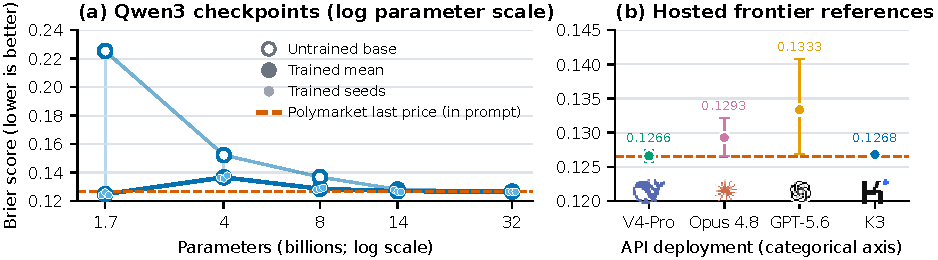
\includegraphics[width=\linewidth]{figures/exp4_qwen_scale_results.pdf}
\captionof{figure}{\textbf{Qwen scaling and hosted frontier references.}
Left: base/trained means and seeds on a log parameter axis. Right: clustered
95\% intervals versus contemporaneous Polymarket; Brier scales differ.}
\label{fig:exp4-scale-results}
\end{minipage}
\end{center}

\textbf{Scale profile.}
Qwen3 trained/base means are $.1248/.2253$, $.1366/.1522$, $.1286/.1369$,
$.1270/.1281$, and $.1265/.1266$ at 1.7B/4B/8B/14B/32B. Across the dense
4B--32B series, the gap contracts as bases approach the trained frontier. The
Llama replication shows the same qualitative trend: the larger base improves
and training approaches the same frontier
(Figure~\ref{fig:exp4-llama-scale-results}). This is consistent with pretraining
and outcome training providing partly substitutable routes to out-of-family
forecast accuracy; Brier scores alone cannot show that they recover the same
relationships.

\textbf{Scale-comparison limits.}
At 32B, trained-minus-base is $-.00007$ $[-.00045,+.00029]$ and trained
minus the contemporaneous crowd (Brier $.12655$) is $-.00003$
$[-.00009,+.00002]$; both intervals cross zero. Thus base scaling, not a larger
marginal training gain, drives convergence under this recipe. Optimization was
not size-tuned and Qwen is nonmonotone; the results establish neither crowd
superiority nor a universal scaling law.


\section{Limitations}
\label{sec:limitations}

\textbf{Behavior does not identify internal computation.}
Experiment~1 is compatible with semantic polarity classification followed by a
learned update size. A label-conditioned analogical regression matches Coin City.
In Experiment~3, lower forecast error coexists with near-chance mechanism labels.
The experiments establish specific input--output behavior but remain compatible
with several internal algorithms and representations.

\textbf{The evaluated environments remain limited.}
The prospective evidence packets are generated and usually state their direction;
the seven-reviewer packet ratings fall short of the registered agreement thresholds,
and the nine-reviewer extension remains incomplete. Experiment~2 uses two
well-separated linear response regimes and a cue that is correct or inverted; its
arbitrary-symbol control covers one deployment. Experiment~3 trains on one direct
Coin City family and evaluates one held-out mediated family in two surface domains.
Its hints are correct, absent, or misleading, but remain categorical descriptions
from a fixed template. The appendix composition study adds unseen nonlinear and
temporal compositions and parameter extrapolation, but every world comes from a
finite catalog and shared prompt format. We do not test graded cue reliability,
ambiguous mechanisms, or new sets of variables.

\textbf{The Coin City model comparison remains incomplete.}
The Coin City result covers Qwen3-4B at the registered round-300 checkpoint under
both greedy and five-draw stochastic decoding, but its Qwen3-8B and Llama-3.1-8B
endpoints were incomplete when this analysis was finalized. The separate
broad-composition study includes all three models and finds heterogeneous
causal-versus-prior effects rather than a roster-wide advantage. Both studies use
one LoRA/Dr.~GRPO recipe and three seeds per arm, and five draws do not
characterize the full output distribution.

\textbf{The market studies have separate validity constraints.}
The unresolved-market interventions cannot be scored against outcomes, and their
evidence packets are hypothetical. Historical markets use one 30-day cutoff and
selected binary domains. Pretraining exposure cannot be audited, archived text
does not include edit histories, and the update analysis fixes the initial
forecast. Historical training improves on the base model but is not statistically distinguishable
from contemporaneous market prices.

\section{Conclusion}
\label{sec:conclusion}

Forecast accuracy alone does not establish inductive reasoning. Models select
relevant evidence and revise contextual relationships, while training improves
forecasts across domains and held-out markets. A supervised pilot learns
response-form selection in distribution but fails to transfer across domains or
arbitrary labels. Composition accuracy exceeds a fixed prior without establishing
transferred evidence use. These contrasts distinguish predictive accuracy from
reliable relationship use without presuming a general world model.

\section*{Acknowledgements}
Acknowledgements are redacted for double-blind review.


\IfFileExists{ICLR/iclr2026_conference.bib}{
  \bibliographystyle{ICLR/iclr2026_conference}
  \bibliography{ICLR/iclr2026_conference}
}{}

\clearpage
\appendix
\section*{Appendices}
\pdfbookmark[1]{Appendices}{appendix-guide}

The supplement is organized by experiment. A descriptive coin-flip elicitation
precedes the Experiment~1 evidence-response details. Experiment~2 documents
contextual relationship selection and revision, including a linear-probe
representation analysis; Experiments~3--4 document controlled and historical
transfer, replication, structure-selection diagnostics, supervised learnability,
and mechanism evidence use. Shared training details
and the artifact map close the appendix.

% Every entry below is derived from its \label: \ref* supplies the number,
% \nameref* the heading text, and \pageref* the page. Nothing here is typed by
% hand, so the guide cannot drift out of sync with the appendix headings the way
% a hard-coded list does. Adding or reordering an appendix section only requires
% adding its label to the list.
\begingroup
\hypersetup{hidelinks}
\small
\setlength{\parskip}{0pt}
\makeatletter
\newcommand{\appendixguidechapter}[1]{%
  \par\addvspace{0.45\baselineskip}%
  \noindent\hyperref[#1]{\textbf{\makebox[2.8em][l]{\ref*{#1}}\nameref*{#1}}}%
  \nobreak\hfill\nobreak
  \hyperref[#1]{\textbf{\pageref*{#1}}}\par
}
\newcommand{\appendixguidesection}[1]{%
  \@dottedtocline{2}{1.3em}{3.4em}%
    {\hyperref[#1]{\numberline{\ref*{#1}}\nameref*{#1}}}%
    {\hyperref[#1]{\pageref*{#1}}}%
}
\makeatother


\appendixguidechapter{app:carnival-coin-probe}

\appendixguidechapter{app:exp1}
\appendixguidesection{app:exp1-sample}
\appendixguidesection{app:exp1-protocol}
\appendixguidesection{app:metrics}
\appendixguidesection{app:extended-results}
\appendixguidesection{app:exp1-limitations}
\appendixguidesection{app:fig-code}
\ifdefined\includeContextReversalPilot
\appendixguidesection{app:exp1-context-reversal}
\fi

\appendixguidechapter{app:coin-city}
\appendixguidesection{app:coin-city-design}
\appendixguidesection{app:coin-city-arms}
\appendixguidesection{app:coin-city-execution}
\appendixguidesection{app:coin-city-analysis}
\appendixguidesection{app:coin-city-results}
\appendixguidesection{app:coin-city-mechanistic-probe}
\appendixguidesection{app:coin-city-limitations}

\appendixguidechapter{app:exp3}
\appendixguidesection{app:exp3-coin-structural}
\appendixguidesection{app:exp3-eight-seed}
\appendixguidesection{app:exp3-structure-selection}
\appendixguidesection{app:exp3-components}
\appendixguidesection{app:exp3-learnability}
\appendixguidesection{app:exp3-evidence-use}

\appendixguidechapter{app:exp4}
\appendixguidesection{app:exp3b-results}
\appendixguidesection{app:exp3b-update}

\appendixguidechapter{app:exp3-complete-training-setup}
\appendixguidesection{app:exp3-coin-structural-hparams}

\appendixguidechapter{app:exp3-repro}

\endgroup

% ============================================================
%  APPENDIX — EXPERIMENT 1 FULL DETAILS
%  Place after the main body, e.g. \appendix\section{...}
% ============================================================

\section{Experiment 1: prospective forecast updating}
\label{app:exp1}

Experiment~1 tests whether
forecast revisions follow evidence direction and whether directional packets
produce larger changes than orthogonal packets.
All reported counts refer to parseable records in the frozen consistency report
unless stated otherwise.

The main comparison reports the nine deployments with scale-valid archived
revisions. This appendix retains Qwen~2.5-7B for directional-compliance diagnostics
and documents why its magnitude-based statistics are excluded.

\subsection{Study design, sample, and agent roster}
\label{app:exp1-sample}

\noindent\textbf{Protocol summary.}
Experiment~1 crosses ten forecasting agents with a frozen set of unresolved binary
Polymarket questions.  The study has four stages: (1)~freeze the market sample;
(2)~obtain one or more initial forecasts from each agent; (3)~generate nine synthetic
evidence packets for each of the 100 core markets (three pro-$H_1$, three
anti-$H_1$, and three outcome-orthogonal); and (4)~ask the same agent to revise each
parseable initial forecast after receiving one packet at a time.  The unit of analysis is an \emph{agent $\times$ market $\times$ initial run
$\times$ counterfactual packet} update.  Requested repeat
counts were five initial runs for hosted agents and three for local agents; realized
valid counts are uneven because of provider failures, parsing failures, and targeted
top-ups.  Section~\ref{app:metrics} specifies how those records are normalized and
aggregated.

\subsubsection{Sampling frame and market selection}
\label{app:market-selection}

The primary sampling frame is a Polymarket API snapshot taken on June~9, 2026.
Selection was deterministic given that snapshot.  We retained markets that were
binary, active and unresolved, scheduled to resolve 14--180 days after sampling,
priced strictly between 0.10 and 0.90 on the YES contract, and supported by at least
\$1,000 in USD volume.  A keyword-based relevance filter retained politics,
government, elections, economics, technology, and geopolitics while excluding
sports, cryptocurrency, entertainment, and other out-of-scope topics.  When several
contracts belonged to the same event, we retained the highest-volume contract.

The recorded filter funnel makes the sampling loss explicit.  The snapshot contained
60,989 binary records; 37,386 were active, 8,639 passed the topic filter, 3,570 passed
the resolution-window filter, 1,403 passed the price filter, 839 passed the volume
filter, and event-level deduplication left 436 candidates.  A diversity pass selected
the 100-market core using a cosine-similarity threshold of 0.25 and a maximum of
16 markets per topical bucket.  The frozen core contains 16 global-election,
16 other, 15 Iran-nuclear, 12 U.S.-federal-policy, 10 AI/technology, 9 U.S.
state-election, 7 Russia--Ukraine, 5 Brazil, 5 U.S.-midterm, 3 macroeconomic,
and 2 China--Taiwan markets.

Counterfactual generation and Stage~3 updating target this 100-market core for
every model, but per-model coverage of it is not uniform. Llama~3.1-70B has 99
analyzable markets because one market has no parseable initial forecast, and
Claude Opus~4.8 has usable updates on all three packet arms in 73 markets;
Section~\ref{app:exp1-alternatives} reports the coverage table and the resulting
robustness checks.

\begin{center}
\begin{minipage}{\linewidth}
\centering
\captionof{table}{Representative markets from the frozen 100-market core.
Snapshot mid is the stored YES midpoint on June~9, 2026 rather than an eventual
outcome.}
\label{tab:markets}
\footnotesize
\resizebox{\linewidth}{!}{%
\begin{tabular}{llc}
\toprule
\textbf{Question} & \textbf{Topic} & \textbf{Snapshot mid} \\
\midrule
Will Renan Santos win the 2026 Brazilian presidential election? & Brazil & 0.17 \\
US--Iran nuclear deal by June~30? & Middle East & 0.20 \\
US $\times$ Iran permanent peace deal by July~31, 2026? & Iran & 0.32 \\
Will a new Gemini flagship be released by June~30, 2026? & AI/technology & 0.89 \\
\bottomrule
\end{tabular}%
}
\end{minipage}
\end{center}

\subsubsection{Agent roster and execution modes}
\label{app:agent-roster}

The roster comprises three hosted API systems and seven open-weight local systems
(Table~\ref{tab:agent-roster}).  The hosted models ran through Azure AI~Foundry and used
its native search-supported Responses workflow \citep{microsoft2026foundry}.  Local
models were served by Ollama \citep{ollama2026} on cluster GPUs; their research turn was supplied by Tavily search.  All agents received the same substantive three-step contract: build an event
model, gather current evidence, and emit a structured forecast. Provider-specific
search orchestration and model runtimes were not identical.

\begin{center}
\begin{minipage}{\linewidth}
\centering
\captionof{table}{Experiment~1 agent roster and requested initial-forecast repeats.  Requested
$k$ is the collection target rather than an analysis denominator; exact realized coverage
appears in Table~\ref{tab:model-summary}.}
\label{tab:agent-roster}
\small
\begin{tabular}{llllc}
\toprule
\textbf{Model} & \textbf{Runtime} & \textbf{Research search} &
\textbf{Nominal params} & \textbf{Requested $k$} \\
\midrule
GPT-5.4          & Azure Foundry & Foundry native & --- & 5 \\
Claude Opus~4.8  & Azure Foundry & Foundry native & --- & 5 \\
DeepSeek V4-Pro  & Azure Foundry & Foundry native & --- & 5 \\
Qwen~2.5-7B      & Ollama & Tavily & 7B  & 3 \\
Qwen~2.5-14B     & Ollama & Tavily & 14B & 3 \\
Qwen~2.5-32B     & Ollama & Tavily & 32B & 3 \\
Qwen~2.5-72B     & Ollama & Tavily & 72B & 3 \\
Llama~3.1-8B     & Ollama & Tavily & 8B  & 3 \\
Llama~3.1-70B    & Ollama & Tavily & 70B & 3 \\
Llama~3.3-70B    & Ollama & Tavily & 70B & 3 \\
\bottomrule
\end{tabular}
\end{minipage}
\end{center}

For local models, reasoning calls used the frozen configuration temperature of 0.1 and
the final JSON-formatting call used temperature 0.0.  Search queries, tool responses,
token counts, parse errors, and provider errors were retained with each run.  Some
smaller models returned probabilities on a 0--100 rather than 0--1 scale.  The
initial-forecast parser converted those values, but the frozen Stage~3 data retain a
mixed-scale Qwen~2.5-7B subset documented in
Section~\ref{app:record-processing}.

\subsection{Forecast, intervention, and validation protocol}
\label{app:exp1-protocol}

\subsubsection{Initial forecast elicitation}
\label{app:prompts}

\noindent\textbf{Design rationale.}
The elicitation asks each agent to restate the resolution criterion, construct
explicit YES and NO hypotheses, identify a status-quo trajectory, research
current evidence, and map its final YES probability to the posterior assigned to
$H_1$. Question restatement and status-quo anchoring follow prior
forecasting-prompt evidence \citep{halawi2024approaching,wilson2025automated}.

\noindent\textbf{Executed three-turn sequence.}
Every frozen initial forecast followed the same substantive sequence, with
provider-specific tool plumbing:

\begin{enumerate}
  \item \textbf{Event model.}  The agent received the question, full resolution
        description, days to resolution, and category.  It restated what would count
        as YES versus NO; identified actors, mechanisms, and latent variables; formed
        $H_1$ (YES) and $H_2$ (NO); and described the status-quo outcome.
  \item \textbf{Current-evidence research.}  The agent gathered evidence for and
        against each hypothesis, checked whether the required chain of events was
        plausible within the remaining time, and revised its assessment.  Hosted
        systems used Azure Foundry's native search workflow; local systems generated
        queries that were executed through Tavily and received the returned evidence
        in context.
  \item \textbf{Structured forecast.}  A final call converted the accumulated analysis
        to the common JSON contract below.  A run entered downstream processing only
        when this object was parseable.
\end{enumerate}

The research turn included this calibration instruction:

\begin{small}
\begin{verbatim}
Given the days remaining, what chain of events is required for H1, and
is that pace of change plausible? Give extra weight to the status quo;
depart substantially only when concrete directional evidence warrants it.
\end{verbatim}
\end{small}

The common output contract was:

\begin{small}
\begin{verbatim}
{
  "event_model": {
    "key_actors": [str],
    "key_mechanisms": [str],
    "latent_variables": [str]
  },
  "hypotheses": [
    {"id": "H1", "description": str,
     "prior_probability": float, "posterior_probability": float,
     "supporting_evidence": [str], "contradicting_evidence": [str]},
    {"id": "H2", ...}
  ],
  "hypothesis_to_forecast_mapping": str,
  "yes_prob": float,
  "confidence": "low"|"medium"|"high",
  "rationale": str,
  "evidence_sources": [str]
}
\end{verbatim}
\end{small}

The contract makes the intended invariant explicit: \(\hat p=P(H_1)\).  The ICS
metric tests whether the returned fields obey that invariant after an intervention.
The substantive prompt contract was common, but prompts were not byte-identical across
runtimes because the hosted and local search interfaces require different orchestration.

\subsubsection{Counterfactual packet construction and validation}
\label{app:cf-taxonomy}

For each of the 100 core markets, GPT-5.4 generated nine synthetic evidence packets:
three pro-$H_1$, three anti-$H_1$, and three orthogonal.  Each generation call received
the market question, resolution description, and a canonical parseable initial event
model and forecast.  It produced:

\begin{itemize}
  \item \textbf{evidence\_headline}: one sentence that states the new development;
  \item \textbf{evidence\_text}: a 2--4 sentence synthetic wire-style item;
  \item \textbf{mechanism\_targeted}: the causal pathway by which the item should
        affect, or remain irrelevant to, resolution;
  \item \textbf{direction}: \texttt{pro\_H1}, \texttt{anti\_H1}, or
        \texttt{orthogonal};
  \item \textbf{slot\_type}: one of the six roles in
        Table~\ref{tab:slot-taxonomy}; and
  \item \textbf{plausibility\_rating}: the generator's 1--5 self-rating.
\end{itemize}

Within each direction, sequential exclusion required a new packet to target a different
actor and mechanism from earlier packets.  Search was disabled so the packets remained
controlled synthetic premises rather than paraphrases of live reporting.

\begin{center}
\begin{minipage}{\linewidth}
\centering
\captionof{table}{Counterfactual slot taxonomy.  Each market receives one packet of every
direction--slot combination shown, for nine packets total.}
\label{tab:slot-taxonomy}
\small
\begin{tabular}{p{2.5cm} p{1.8cm} p{7.5cm}}
\toprule
\textbf{Slot type} & \textbf{Direction} & \textbf{Role in the intervention} \\
\midrule
DATA        & pro, anti & A measurement, price signal, statistic, or poll that
               shifts the likelihood of $H_1$. \\
DECISION    & pro, anti & An actor decision, official statement, policy announcement,
               commitment, or refusal bearing on $H_1$. \\
STRUCTURAL  & pro, anti & A technical, logistical, legal, or contextual change that
               makes $H_1$ more or less likely. \\
PROCEDURAL  & orthogonal & A same-domain administrative or process update without a
               direct causal path to $H_1$ versus $H_2$. \\
PERSONNEL   & orthogonal & A staffing or leadership change involving a relevant actor
               but an issue unrelated to $H_1$ versus $H_2$. \\
BACKDROP    & orthogonal & Contextual economic, logistical, or social information that
               sets the scene without shifting the outcome odds. \\
\bottomrule
\end{tabular}
\end{minipage}
\end{center}

\noindent\textbf{Packet-level integrity checks.}
The frozen packet file contains 900/900 parseable records: 100 markets multiplied by
nine packets, with exactly 300 pro-$H_1$, 300 anti-$H_1$, and 300 orthogonal records.
Every packet has a nonempty headline, and the logs contain zero search calls.  All 900
generator-assigned plausibility ratings equal 4/5. That field documents the
generator's compliance claim but provides neither variation nor independent
validation; the separate human materials review is reported below.
These checks verify structural completeness; they do not establish that directional
strength or difficulty is perfectly matched across packets.

As an illustration, for the Hormuz market the pro-$H_1$ headline
\textit{Oman says Iran agrees daily protected windows for commercial Hormuz transits}
elicited the largest single update reported in the viewer: Claude Opus~4.8 revised
from 10\% to 45\% (\(\Delta\hat p=+35\)~pp).  The orthogonal IMO
incident-reporting item produced negligible movement.

\subsubsection{Stage~3 update and pairing}
\label{app:update-protocol}

Each packet was presented separately with the agent's own parseable initial structured
forecast.  The agent was told to reason only from that forecast and the packet and to
return the same structured forecast with revised $H_1$, $H_2$, and YES probabilities.
Search was disabled.

\noindent\textbf{One deployment received an extra instruction.}
The Stage~3 template was not common across the roster.  GPT-5.4 alone was run with the
runner's \texttt{novelty} option, which appends a rule asking for a
\texttt{novelty\_assessment}: \emph{a single sentence stating whether this evidence was
likely already reflected in your initial forecast as background knowledge (suggesting a
small update) or is genuinely new and surprising (warranting a larger revision)}.
The frozen records show the asymmetry exactly: 3{,}838 of 3{,}921 GPT-5.4 updates carry
the field and no other deployment carries it in any record.  The instruction tells a
model to modulate revision size by perceived novelty, which is close to the construct
Section~\ref{app:exp1-alternatives} estimates, and GPT-5.4 is the deployment that
behaves differently on exactly that dimension: it returns the prior unchanged on
$8.4\%$ of orthogonal packets against $71.4\%$ and $44.4\%$ for the other two hosted
systems, writing a small revision where they abstain.  We cannot separate that
difference from the prompt difference, so GPT-5.4's abstention rate is not comparable to
the rest of the roster and we do not read the hosted ordering on abstention as a model
difference.  Its conditional magnitude, directional correctness, and AUC use the same
scoring as every other deployment.

For an agent--market cell with \(k\) parseable initial runs, the intended crossed design
contains \(9k\) update records.  Each update is conditionally independent in prompt
context: it contains one initial run and one packet, never another packet or another
agent's answer.  The novelty field is not a reported endpoint and should not be
viewed as a validated correction.

Provider interruptions, parse failures, and subsequent top-ups make realized cells
uneven.  We therefore report exact valid record and market denominators by model in
Table~\ref{tab:model-summary} rather than treating requested \(k\) or the theoretical
\(9k\) as observed sample sizes.

\subsection{Estimands, record processing, and aggregation}
\label{app:metrics}

\subsubsection{Record construction, deduplication, and missingness}
\label{app:record-processing}

The frozen analysis artifact is
\path{exp1_prospective/data/results/consistency_report_2026-06-17.json}; tables in
this paper use its stored denominators rather than a fresh scan of the evolving
collection directories.  During report construction, date suffixes are stripped from
task identifiers so daily collection files join to the same market.  Counterfactuals
are deduplicated by \texttt{cf\_id}; updates are deduplicated by
\texttt{update\_id}, with a parseable record preferred over an error record when both
exist.  Files are read newest first for the initial-forecast and market-price lookup.
Malformed JSON lines are skipped.  Missing values are handled per estimand: a record
may therefore contribute to ICS but not EHC, or vice versa, depending on which fields
parse.

Stage~3 update fields were evaluated on their stored scale in the frozen report.
For Qwen~2.5-7B, 207 of 8,636 deduplicated records store
\texttt{updated\_yes\_prob} above 1.5; no other model does. Its directional sign
metrics remain usable, but its absolute revision magnitudes and sensitivity
ratio are scale-contaminated and are omitted from the paper tables.

\subsubsection{Consistency estimands}
\label{app:metric-definitions}

For update record \(i\), let \(d_i\in\{+1,-1\}\) denote the intended direction
(\(+1\) for pro-$H_1$, \(-1\) for anti-$H_1$).  Orthogonal packets do not have an
intended sign and are excluded from EHC and HFC.  The 3~pp movement threshold excludes
cases in which a model effectively leaves the forecast unchanged.

\noindent\textbf{Evidence--hypothesis consistency (EHC).}
Let \(\Delta p(H_1)_i=p(H_1)_i^{\mathrm{post}}-\hat p_i^{\mathrm{initial}}\).
For directional records with \(|\Delta p(H_1)_i|\geq0.03\),
\begin{equation}
  \mathrm{EHC}_i=\mathbf{1}\!\left[\Delta p(H_1)_i d_i>0\right].
  \label{eq:ehc}
\end{equation}
EHC asks whether the updated hypothesis field moves in the direction implied by the
packet; it does not score the size of that movement.

\noindent\textbf{Hypothesis--forecast consistency (HFC).}
Let \(\Delta\hat p_i=\hat p_i^{\mathrm{post}}-\hat p_i^{\mathrm{initial}}\).
For directional records with \(|\Delta\hat p_i|\geq0.03\),
\begin{equation}
  \mathrm{HFC}_i=\mathbf{1}\!\left[\Delta\hat p_i d_i>0\right].
  \label{eq:hfc}
\end{equation}
HFC asks the same directional question of the headline YES probability. Because
the output contract requires this probability to equal $P(H_1)$, we retain HFC in
the appendix as a compliance diagnostic rather than as a separate main-text result.

\noindent\textbf{Internal coherence score (ICS).}
ICS is defined whenever both updated fields parse and is unconditional on movement:
\begin{equation}
  \mathrm{ICS}_i=\mathbf{1}\!\left[
  \left|\hat p_i^{\mathrm{post}}-p(H_1)_i^{\mathrm{post}}\right|<0.02\right].
  \label{eq:ics}
\end{equation}
The inequality is strict: a discrepancy of exactly 2~pp does not pass.

\noindent\textbf{Directional sensitivity.}
Packet selectivity is summarized by
\begin{equation}
  \mathrm{Sensitivity}=
  \frac{\overline{|\Delta\hat p|}_{\mathrm{pro}+\mathrm{anti}}}
       {\overline{|\Delta\hat p|}_{\mathrm{orthogonal}}}.
  \label{eq:sensitivity}
\end{equation}
A value near one indicates comparable movement for directional and orthogonal
packets; larger values indicate preferential response to directional packets. This
ratio is descriptive.  It cancels a uniform multiplicative scale within a model, but
does not repair mixed scales across records, hence the Qwen~2.5-7B caveat above.

\subsubsection{Aggregation and uncertainty}
\label{app:aggregation}

For EHC, HFC, and ICS, the evaluator first pools eligible records within each
model--market cell to obtain a market-level rate.  The reported model score is the
unweighted mean of those market rates, so a market with more successful repeat runs
does not receive greater weight.  Reported standard errors are the sample standard
deviation of market-level rates divided by the square root of the number of markets.

Revision magnitudes and sensitivity retain the record-pooled point estimands.
Uncertainty uses 20,000 percentile cluster-bootstrap draws over represented markets.
All nine packets and every repeated initial-run update from a selected market remain
together, and sensitivity is recomputed from pooled directional and orthogonal
movement within each draw. This accounts for dependence among records from the same
market while preserving the published estimand.

\subsubsection{Output compliance and threshold robustness}
\label{app:exp1-threshold-robustness}

\noindent\textbf{Output-field coupling.}
The final-output schema explicitly instructs the agent that
$\hat p=P(H_1)$, and the Stage~3 prompt requests the same structure after
updating. EHC and HFC are therefore not independent tests of an inferred
hypothesis-to-forecast link. ICS is a schema-adherence diagnostic, while close
EHC--HFC agreement reflects a mixture of directional updating and compliance
with the prompted equality. Among the 26,010 relevant records with both updated
fields present, 25,984 (99.90\%) satisfy the equality exactly after scale
normalisation and 25,987 (99.91\%) satisfy it within the 2-pp ICS tolerance. We
therefore do not treat EHC--HFC parity as independent evidence for a latent
representation or for spontaneous propagation between separately elicited
quantities.

\noindent\textbf{Unconditional estimand.}
For threshold $t$, Table~\ref{tab:exp1-threshold-robustness} retains a valid
directional update when $|\Delta|\geq t$ and reports the fraction for which
$d_i\Delta_i>0$. At $t=0$, every valid pro- and anti-$H_1$ update enters the
denominator and a zero change is scored incorrect. We first compute correctness
within market and then average markets equally, matching the primary analysis.
The \emph{Below 3 pp} column is the record-weighted fraction and count excluded
by the published 3-pp conditional metric. The table's $n$ is the complete
pre-threshold denominator: records require a parseable initial probability and
the applicable updated field, but are not selected on the direction or magnitude
of movement.

\begin{center}
\begin{minipage}{\linewidth}
\centering
\captionof{table}{Unconditional directional correctness and robustness to 0-,
1-, 3-, and 5-percentage-point movement thresholds. The 0-pp column is
unconditional over all valid directional updates and scores zero movement as
incorrect; positive-threshold columns condition on the stated magnitude.
\emph{Below 3 pp} gives the percentage and count omitted from the corresponding
published 3-pp EHC or HFC denominator. Rates are macro-averaged across markets.}
\label{tab:exp1-threshold-robustness}
\scriptsize
\setlength{\tabcolsep}{4pt}
\resizebox{\linewidth}{!}{%
% Generated by exp1_prospective/agent/evaluate_threshold_robustness.py
\begin{tabular}{llrrrrrr}
\toprule
& & & \multicolumn{4}{c}{Directional correctness} & \\
\cmidrule(lr){4-7}
\textbf{Model} & \textbf{Metric} & \textbf{$n$ valid} &
\textbf{0 pp} & \textbf{1 pp} & \textbf{3 pp} & \textbf{5 pp} &
\textbf{Below 3 pp} \\
\midrule
Claude Opus~4.8 & EHC & 2,119 & 98.2\% & 98.6\% & 99.0\% & 99.5\% & 18.1\% (383) \\
 & HFC & 2,119 & 98.3\% & 98.6\% & 99.0\% & 99.5\% & 18.1\% (383) \\
GPT-5.4 & EHC & 2,678 & 98.4\% & 98.4\% & 98.7\% & 98.8\% & 6.9\% (185) \\
 & HFC & 2,684 & 98.4\% & 98.4\% & 98.7\% & 98.8\% & 6.9\% (185) \\
DeepSeek V4-Pro & EHC & 2,929 & 97.3\% & 97.6\% & 97.7\% & 98.0\% & 12.7\% (371) \\
 & HFC & 2,929 & 97.3\% & 97.6\% & 97.7\% & 98.0\% & 12.6\% (370) \\
\midrule
Llama~3.3-70B & EHC & 1,788 & 96.4\% & 96.4\% & 96.5\% & 97.4\% & 0.7\% (12) \\
 & HFC & 1,788 & 96.4\% & 96.4\% & 96.5\% & 97.4\% & 0.7\% (12) \\
Llama~3.1-70B & EHC & 1,659 & 96.1\% & 96.1\% & 96.1\% & 96.7\% & 0.6\% (10) \\
 & HFC & 1,659 & 96.1\% & 96.1\% & 96.1\% & 96.7\% & 0.6\% (10) \\
Qwen~2.5-72B & EHC & 1,795 & 96.3\% & 96.3\% & 96.3\% & 96.4\% & 0.8\% (15) \\
 & HFC & 1,795 & 96.3\% & 96.3\% & 96.3\% & 96.4\% & 0.8\% (15) \\
Qwen~2.5-32B & EHC & 1,795 & 96.4\% & 96.4\% & 96.4\% & 96.5\% & 1.9\% (34) \\
 & HFC & 1,795 & 96.4\% & 96.4\% & 96.4\% & 96.5\% & 1.9\% (34) \\
Qwen~2.5-14B & EHC & 1,800 & 93.1\% & 94.4\% & 94.3\% & 94.3\% & 2.9\% (52) \\
 & HFC & 1,800 & 93.1\% & 94.4\% & 94.3\% & 94.3\% & 2.9\% (52) \\
Qwen~2.5-7B & EHC & 5,759 & 90.2\% & 90.2\% & 90.6\% & 90.8\% & 2.2\% (129) \\
 & HFC & 5,759 & 89.9\% & 90.2\% & 90.5\% & 90.8\% & 2.4\% (140) \\
Llama~3.1-8B & EHC & 3,601 & 88.1\% & 88.7\% & 88.7\% & 88.9\% & 1.7\% (62) \\
 & HFC & 3,604 & 88.4\% & 88.7\% & 88.7\% & 88.9\% & 1.4\% (52) \\
\bottomrule
\end{tabular}

}
\end{minipage}
\end{center}

\noindent\textbf{Threshold-sweep results.}
The threshold sweep preserves the qualitative conclusion but narrows its
wording. Hosted-model unconditional correctness is 97.3--98.4\%; at the
published 3-pp threshold it is 97.7--99.0\%. The 3-pp rule excludes 6.9\% of
GPT-5.4, 12.6--12.7\% of DeepSeek V4-Pro, and 18.1\% of Claude Opus~4.8
directional updates. Thus, the near-1.0 EHC/HFC values do not result from
discarding a majority of cases, and the conclusion is stable across 0, 1, 3,
and 5~pp. The precise statement is \emph{99\% directionally correct among updates
of at least 3~pp}. It is not \emph{99\% coherent updating}. Small local
models have fewer sub-3-pp updates (0.6--2.9\%) but lower unconditional
correctness (88.1--96.4\%), so their errors are not hidden primarily by the
movement filter.

\noindent\textbf{Normalisation and reproducibility.}
Before recomputing deltas, the analysis independently normalises the initial
headline probability, updated headline probability, and updated $H_1$
posterior from the documented $[0,1]$ or $[0,100]$ formats. This matters for
166 relevant Llama~3.1-8B records in which $H_1$ was emitted as a percentage
while \texttt{yes\_prob} was emitted as a proportion. The complete eligible
record and market counts at every threshold, invalid-field counts, market-level
standard errors, input-file SHA-256 hashes, and full-precision estimates are in
\path{exp1_prospective/data/results/threshold_robustness.json}. The table is
regenerated by
\path{exp1_prospective/agent/evaluate_threshold_robustness.py}; neither script
nor table filters items using realized outcomes.

\subsection{Extended results}
\label{app:extended-results}

\subsubsection{Analysis coverage}
Table~\ref{tab:model-summary} gives the exact Stage~3 record and market counts.
The market column counts markets with at least one valid update. Coverage of all
three packet arms is not uniform across models: Llama~3.1-70B has 99 analyzable
markets because one market has no parseable initial forecast, and Claude Opus~4.8
has all three arms in 73 of 100. Section~\ref{app:exp1-alternatives} gives the
per-arm coverage and assesses whether missingness is arm-selective.

\begin{center}
\begin{minipage}{\linewidth}
\centering
\captionof{table}{Valid Stage~3 update records and represented core markets by
agent.  Hosted systems first; open-weight rows in descending parameter count.}
\label{tab:model-summary}
\small
\begin{tabular}{llrr}
\toprule
\textbf{Model} & \textbf{Type} & \textbf{Records} & \textbf{Markets} \\
\midrule
Claude Opus~4.8 & Hosted  & 3{,}125 & 100 \\
GPT-5.4         & Hosted  & 3{,}913 & 100 \\
DeepSeek V4-Pro & Hosted  & 4{,}395 & 100 \\
Qwen~2.5-72B    & Local 72B & 2{,}692 & 100 \\
Llama~3.3-70B   & Local 70B & 2{,}682 & 100 \\
Llama~3.1-70B   & Local 70B & 2{,}490 &  99 \\
Qwen~2.5-32B    & Local 32B & 2{,}693 & 100 \\
Qwen~2.5-14B    & Local 14B & 2{,}700 & 100 \\
Llama~3.1-8B    & Local 8B  & 5{,}404 & 100 \\
Qwen~2.5-7B     & Local 7B  & 8{,}636 & 100 \\
\midrule
\textbf{Total}  &           & \textbf{38{,}730} & \\
\bottomrule
\end{tabular}
\end{minipage}
\end{center}

\subsubsection{Prospective settlement audit}
\label{app:exp1-outcome-followup}

The frozen-cohort evaluation includes a dated settlement audit that leaves the
directional-updating estimand unchanged. On August~24, 2026, we queried the public
Polymarket market endpoint for the exact 100 frozen IDs. We admitted a label only
when the market was closed and the YES/NO token prices were exactly
\([1,0]\) or \([0,1]\).  This strict rule yielded 60 scoreable markets
(21 YES and 39 NO). One additional closed market had an invalid \(0.5/0.5\)
settlement and 39 remained unresolved at the audit cutoff; all 40 were excluded.

For each agent--market cell, the forecast is the median of its parseable repeated
initial YES probabilities, matching the maintained Experiment~1 viewer.  The crowd
benchmark is the YES price stored in the frozen June~9 selection record.  We report
threshold accuracy (YES iff \(p>0.5\)), Brier score, and natural-log loss.  Proper-score
contrasts are paired agent-minus-market differences; negative values favor the
agent.  Percentile intervals use 20,000 market-level bootstrap resamples.

\begin{center}
\begin{minipage}{\linewidth}
\centering
\captionof{table}{Descriptive accuracy on the first 60 strictly settled markets.
A/M denotes agent/June~9 market on the same rows; Correct is the number of
thresholded calls matching the outcome.  Lower Brier and log loss are better, and
each \(\Delta\) is agent minus market.  Llama~3.1-70B lacks a parseable initial
forecast for one settled market, so its paired denominator is 59.}
\label{tab:exp1-resolved-outcomes}
\scriptsize
\resizebox{\linewidth}{!}{%
% Generated by exp1_prospective/agent/evaluate_resolved_outcomes.py
\begin{tabular}{lrrrrrr}
\toprule
\textbf{Model} & \textbf{$n$} & \textbf{Correct A/M} & \textbf{Brier A/M} & \textbf{$\Delta$Brier [95\% CI]} & \textbf{Log A/M} & \textbf{$\Delta$log [95\% CI]} \\
\midrule
Claude Opus~4.8 & 60 & 41/39 & $.242/.246$ & $-.004 [-.063,.054]$ & $.738/.700$ & $.038 [-.129,.210]$ \\
GPT-5.4 & 60 & 40/39 & $.225/.246$ & $-.021 [-.074,.030]$ & $.663/.700$ & $-.037 [-.178,.103]$ \\
DeepSeek V4-Pro & 60 & 40/39 & $.257/.246$ & $.011 [-.050,.069]$ & $.793/.700$ & $.093 [-.093,.282]$ \\
\midrule
Qwen2.5-72B & 60 & 32/39 & $.265/.246$ & $.019 [-.031,.066]$ & $.728/.700$ & $.028 [-.097,.144]$ \\
Llama-3.3-70B & 60 & 30/39 & $.266/.246$ & $.020 [-.038,.078]$ & $.732/.700$ & $.032 [-.113,.177]$ \\
Llama-3.1-70B & 59 & 33/38 & $.258/.249$ & $.008 [-.058,.075]$ & $.712/.707$ & $.004 [-.155,.164]$ \\
Qwen2.5-32B & 60 & 32/39 & $.264/.246$ & $.018 [-.044,.078]$ & $.728/.700$ & $.028 [-.126,.178]$ \\
Qwen2.5-14B & 60 & 37/39 & $.277/.246$ & $.031 [-.031,.092]$ & $.827/.700$ & $.127 [-.049,.308]$ \\
Llama-3.1-8B & 60 & 31/39 & $.266/.246$ & $.020 [-.047,.085]$ & $.741/.700$ & $.041 [-.127,.202]$ \\
Qwen2.5-7B & 60 & 38/39 & $.230/.246$ & $-.016 [-.075,.041]$ & $.651/.700$ & $-.049 [-.195,.090]$ \\
\bottomrule
\end{tabular}

}
\end{minipage}
\end{center}

The raw correct-call counts are close for the hosted agents and crowd:
Claude Opus~4.8 gets 41/60 correct, GPT-5.4 and DeepSeek V4-Pro each get
40/60, and the June~9 market side gets 39/60.  GPT-5.4 has the lowest Brier
score (\(.225\) versus \(.246\) for the market), a paired difference of
\(-.021\;[-.074,.030]\); its log-loss difference is
\(-.037\;[-.178,.103]\).  Qwen~2.5-7B has the lowest log loss (\(.651\)
versus \(.700\)), but gets 38/60 thresholded calls correct.  No agent's paired
Brier or log-loss interval excludes zero.

This audit describes the outcome-ready slice of the frozen cohort. Settlement by
the audit date censors the cohort toward shorter-horizon and early-resolving
questions, so the 60 are not a random subset of the frozen 100.  Moreover, the
benchmark is the June~9 snapshot whereas agent forecasts were collected from
June~10 through June~17; later-running agents may have had additional public
information.  The result therefore does not establish superiority to the crowd.
It documents the prospective check; the directional-update estimates do not, by
themselves, imply a detectable accuracy advantage.

\subsubsection{Revision magnitudes and packet selectivity}
Table~\ref{tab:anchoring} reports mean absolute forecast revision
\(\overline{|\Delta\hat p|}\) by packet direction.  For the nine models whose updates
are consistently stored on 0--1, hosted-system sensitivity is $8.2$--$24.0\times$,
compared with $1.9$--$6.4\times$ for local systems. These are the unconditional
ratios; Table~\ref{tab:exp1-abstention} separates the abstention and magnitude
factors behind them, and the main text reports those two rather than the product.

Qwen~2.5-7B has mixed 0--1 and 0--100 stored updates
(Section~\ref{app:record-processing}); we therefore omit its absolute magnitudes
and sensitivity ratio rather than present them as comparable estimates.

\begin{center}
\begin{minipage}{\linewidth}
\centering
\captionof{table}{Mean absolute forecast revision by counterfactual direction.
Hosted systems first; open-weight rows in descending parameter count.
Sensitivity is mean directional divided by mean orthogonal movement; \(n\) is the
valid Stage~3 record count. Values are percentage points for models with
consistently stored 0--1 updates.}
\label{tab:anchoring}
\small
\begin{tabular}{llccccc}
\toprule
\textbf{Model} & \textbf{Type} & pro-$H_1$ & anti-$H_1$ & orthogonal
  & \textbf{Sensitivity} & $n$ \\
\midrule
Claude Opus~4.8 & Hosted  & 12.7\,pp & 9.6\,pp  & 0.5\,pp & $24.0\times$ & 3{,}125 \\
DeepSeek V4-Pro & Hosted  & 13.9\,pp & 11.4\,pp & 1.4\,pp & $8.9\times$  & 4{,}395 \\
GPT-5.4         & Hosted  & 10.6\,pp & 8.5\,pp  & 1.2\,pp & $8.2\times$  & 3{,}913 \\
\midrule
Qwen~2.5-72B    & Local 72B & 15.0\,pp & 10.2\,pp & 3.0\,pp & $4.2\times$  & 2{,}692 \\
Llama~3.3-70B   & Local 70B & 14.8\,pp & 14.3\,pp & 2.3\,pp & $6.4\times$  & 2{,}682 \\
Llama~3.1-70B   & Local 70B & 14.8\,pp & 15.5\,pp & 3.3\,pp & $4.6\times$  & 2{,}490 \\
Qwen~2.5-32B    & Local 32B & 15.0\,pp & 10.3\,pp & 4.0\,pp & $3.2\times$  & 2{,}693 \\
Qwen~2.5-14B    & Local 14B & 14.8\,pp &  8.6\,pp & 4.1\,pp & $2.9\times$  & 2{,}700 \\
Llama~3.1-8B    & Local 8B  & 11.1\,pp & 12.0\,pp & 5.9\,pp & $1.9\times$ & 5{,}404 \\
Qwen~2.5-7B     & Local 7B  & --- & --- & --- & --- & 8{,}636 \\
\bottomrule
\end{tabular}
\end{minipage}
\end{center}
Qwen~2.5-7B magnitude cells are omitted because 207 deduplicated updates are
stored above 1.5, mixing probability scales within the row.
Table~\ref{tab:anchoring} documents the magnitude contrast; Figure~\ref{fig:causal-coherent} then places directional consistency and packet selectivity on a common visual scale.

\begin{center}
\begin{minipage}{\linewidth}
\centering
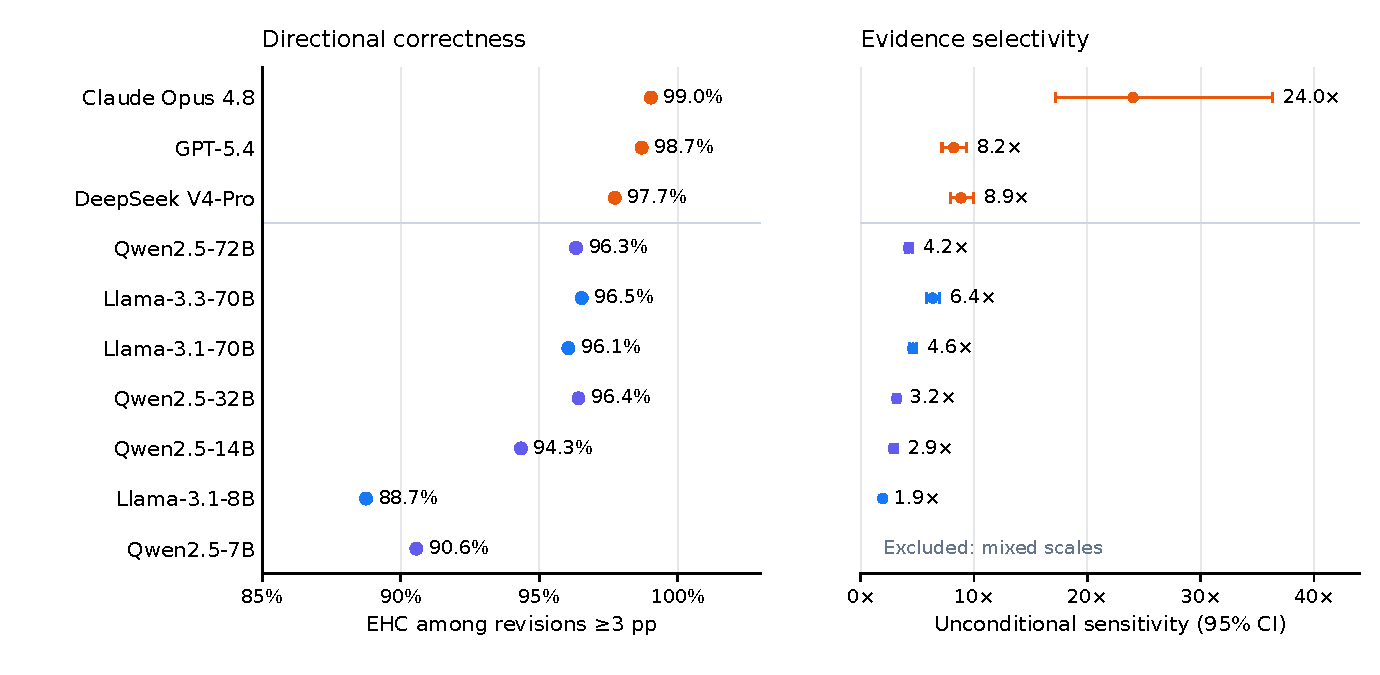
\includegraphics[width=\linewidth]{figures/exp1_ehc_sensitivity_combined.pdf}
\captionof{figure}{\textbf{Directional consistency and packet selectivity by
deployment.} \emph{Left:} EHC is $87$--$90\%$ for 7--8B local models and
$98$--$99\%$ for hosted systems. \emph{Right:} sensitivity is
$1.9$--$6.4\times$ for local models and $8.2$--$24.0\times$ for hosted systems;
Qwen~2.5-7B is omitted from this panel because its archived absolute revisions mix
0--1 and 0--100 scales and therefore do not yield a comparable ratio. The panel
plots the unconditional ratio, which Table~\ref{tab:exp1-abstention} decomposes.}
\label{fig:causal-coherent}
\end{minipage}
\end{center}






\subsection{Study limitations}
\label{app:exp1-limitations}


\subsubsection{Sampling and outcome scope}
The sample is a filtered slice of liquid, medium-horizon Polymarket questions
rather than a probability sample of forecasting tasks. Topic exclusions, the
0.10--0.90 price window, the 14--180 day horizon, event deduplication, and the
diversity cap shape its difficulty distribution.  The primary Experiment~1
estimand evaluates conditional updating on questions that were unresolved at
collection.  The settlement audit in
Section~\ref{app:exp1-outcome-followup} is naturally censored to the first 60
strict settlements and is descriptive.  Experiment~4 separately evaluates
accuracy on a locked sample of resolved historical markets with synchronized
forecast cutoffs and market-price baselines.

\subsubsection{What the update prompt withholds}
\label{app:exp1-withholding}
The Stage~3 template fills in one packet field, \texttt{evidence\_text}. The packet
record also holds the intended \texttt{direction}, \texttt{target\_hypothesis},
\texttt{expected\_hypothesis\_shift}, \texttt{slot\_type}, \texttt{evidence\_headline},
\texttt{mechanism\_targeted}, and a free-text \texttt{rationale}. None of these
reaches the agent; all are read only when the update is scored. The agent sees its
own prior forecast, the snippet, and the fixed instruction.

We checked this two ways. Over the 12{,}728 frozen records that kept their prompt
string, spanning all three hosted systems, the evidence block is identical to the
packet's \texttt{evidence\_text} and contains no private packet field. Prompt
persistence was a per-runner logging choice, so this covers a subset of records by
logging coverage rather than by outcome; the runners that stored nothing use the
same one-field template. Turning to the snippets, none of the 900 names $H_1$,
$H_2$, the market, or its resolution. Twenty-two (2.4\%, 10 pro-$H_1$ and 12
anti-$H_1$) use any likelihood wording---\emph{odds}, \emph{chance of},
\emph{more}/\emph{less likely}, \emph{probability}, \emph{likelihood}---and each
time it describes something in the world, a simulation percentage or a betting
line, not the market's resolution. The sign is not stated; it must be inferred from the relation between the
reported event and the market outcome. Reproduced by
\path{exp1_prospective/agent/audit_packet_polarity.py}.

\subsubsection{Alternative explanations for the selectivity gap}
\label{app:exp1-alternatives}
Here we state the competing accounts of the movement gap and what we find for each.
All checks come from \path{exp1_prospective/agent/audit_selectivity_robustness.py},
\path{audit_orthogonal_abstention.py}, \path{audit_lexical_sign_baseline.py}, and
\path{audit_group_contrast.py}.

\textbf{Where the numbers come from.} The checks read the frozen June~17 report,
which enumerates every scored run, so they use exactly the data behind the
published numbers. The enumeration matches the report's own per-arm counts for
seven of the nine models; Claude Opus~4.8 and GPT-5.4 carry 14 and 4 extra runs in
markets absent from the per-market join, 18 of 38{,}730. Reproduced sensitivity
ratios agree with the published ones to within $0.2$. Three checks need packet
text and so join runs to the June~10 packet set; 346 runs (1.1\%) do not join
because they come from a June~7--8 pilot against a superseded 63-packet
generation, and they are dropped from those three checks only.

\textbf{Attrition is much higher for the hosted systems.} Claude Opus~4.8 made
9{,}313 calls and yielded 3{,}232 usable updates, losing 3{,}656 to broken pipes,
914 to HTTP~401s after a key expired mid-run, and 1{,}481 to unparseable
responses. Of those, 1{,}461 come from one malfunctioning June~15 retry pass that
failed at 91\%; the main June~10 collection parsed at 99.3\%, so the published
compliance figures are not survivorship. DeepSeek~V4-Pro made 6{,}338 calls for
4{,}598 usable updates, losing 1{,}629 to HTTP~401s; GPT-5.4 made 4{,}269 for
4{,}057. The six local models lose almost nothing---four record no failed calls,
the other two lose 8 and 15 responses to parsing. Content-based exclusion is
confined to 28 GPT-5.4 calls across 2 markets. Recorded failures are predominantly
transport or parsing failures; the coverage check below assesses arm and market
imbalance, not content-specific selection. Separately, two
update streams were corrupted by concurrent writes and repaired in August~2026,
after the freeze; the original bytes and unrecoverable fragments sit in
\path{exp1_prospective/data/_recovery_audit/}. Nothing in this section reads those
files.

\textbf{The generator saw one agent's world model.} All packets were built from a
single canonical initial forecast, and it is DeepSeek~V4-Pro's: its June~10 YES
probability matches the stored generation prior on 100 of 100 markets, where no
other agent matches on more than 28. For the other eight models the evidence came
from a different system's event model. The seed model gains nothing by it---among
hosted systems it is second on sensitivity ($8.9\times$ against Claude's
$24.0\times$), third on AUC ($.967$), and last on EHC ($.977$)---but its estimates
are the least independent in the roster.

\textbf{Coverage is uneven across arms.} Table~\ref{tab:exp1-arm-coverage} gives
per-arm market coverage. Seven models cover 99 or 100 markets on every arm. Claude
Opus~4.8 covers 82 on the orthogonal arm and 77 on the directional arms, 73 in
common, so its pooled ratio divides means taken over slightly different market
sets. Restricting to its 73 common markets gives $23.7\times$ against $24.2\times$
pooled. As a proxy check, every other model has similar sensitivity on the markets
Claude covers and those it misses ($8.4$ vs.\
$7.6$ for GPT-5.4, $9.7$ vs.\ $7.2$ for DeepSeek~V4-Pro, $4.3$ vs.\ $4.2$ for
Qwen~2.5-72B, $1.9$ vs.\ $2.1$ for Llama~3.1-8B).

\textbf{The ratio has an unstable denominator.} Claude's orthogonal mean is
$0.5$~pp, so its $24\times$ comes from a small divisor rather than unusually large
directional movement, and its market-clustered interval is correspondingly wide,
$[17.3,36.9]$. Table~\ref{tab:exp1-selectivity-robustness} reports three
statistics that avoid that division. The difference of means is $5.6$--$12.3$~pp
and does not order the models the way the ratio does. The within-market
probability that a directional packet moves the forecast more than an orthogonal
one runs from $.791$ for Llama~3.1-8B to $.994$ for GPT-5.4, putting GPT-5.4 above
Claude Opus~4.8 and reversing the ratio ranking. Every model moves further on
directional packets in every market it covers.

\textbf{The denominator is mostly zeros.} That instability has a specific cause,
and naming it replaces the ratio with two statistics that are easier to read. A
revision of exactly zero---the model reproduces the probability shown to it---enters
the mean like any other record, so the ratio silently mixes how often a
deployment declines to move with how far it moves when it does. Writing $A$ for
the share of runs with $\Delta\hat p=0$ and $M$ for the mean absolute revision
among the rest, $\overline{|\Delta\hat p|}=(1-A)M$, and the ratio factors exactly:
\begin{equation}
  \mathrm{Sensitivity}
  =\underbrace{\frac{M_{\mathrm{dir}}}{M_{\mathrm{orth}}}}_{\text{magnitude}}
  \times\underbrace{\frac{1-A_{\mathrm{dir}}}{1-A_{\mathrm{orth}}}}_{\text{abstention}}.
  \label{eq:sensitivity-decomposition}
\end{equation}
Table~\ref{tab:exp1-abstention} gives both factors. Directional abstention is
$0.0$--$1.4\%$ for every deployment, so the second factor is governed entirely by
the orthogonal arm, where abstention runs from $1.1\%$ for Llama~3.1-8B to
$71.4\%$ $[63.8,78.5]$ for Claude Opus~4.8. Claude's $24\times$ is therefore
$7.0\times$ $[5.5,9.1]$ in magnitude multiplied by $3.48$ in abstention;
DeepSeek~V4-Pro's $8.9\times$ is $4.9\times$ times $1.79$; GPT-5.4's $8.2\times$
is $7.5\times$ times $1.09$, because GPT-5.4 writes a small revision where the
other two hosted systems return the prior unchanged. Across the roster the
published $1.9$--$24.2\times$ becomes $1.9$--$7.5\times$ once the zeros are
separated out, and the ordering changes: GPT-5.4 rather than Claude Opus~4.8 is
highest, and Llama~3.3-70B at $5.7\times$ sits above DeepSeek~V4-Pro at
$4.9\times$.

We report both factors rather than the product. Declining to revise at all is an
appropriate response to an outcome-irrelevant premise, so the abstention rate is
a selectivity measure in its own right and a better-behaved one: it is a bounded
proportion, it is paired within model across arms, and it needs no division by a
small number. It is also the more fragile of the two. An exact copy of a
displayed prior is a discrete act adjacent to formatting, and the update prompt
does instruct the agent to leave unaffected fields unchanged, so we do not read a
high rate as evidence about internal computation. The no-information condition
described in Section~\ref{app:exp1-limitations} is what would separate declining
to revise from copying the anchor, and it was not run. Reproduced by
\path{exp1_prospective/agent/audit_orthogonal_abstention.py}.

\begin{center}
\begin{minipage}{\linewidth}
\centering
\captionof{table}{Decomposition of the sensitivity ratio into magnitude and
abstention factors (Equation~\ref{eq:sensitivity-decomposition}). \emph{Orthogonal
abstention} is the share of orthogonal runs with $\Delta\hat p$ exactly zero; the
directional-arm rate is $0.0$--$1.4\%$ throughout. The two \emph{given a move}
columns condition on a nonzero revision, and their ratio is the magnitude factor.
Brackets are 95\% market-clustered percentile intervals from 20,000 draws, the
scheme used for the published movement intervals. Qwen~2.5-7B is omitted for
mixed probability scales.}
\label{tab:exp1-abstention}
\scriptsize
\setlength{\tabcolsep}{4pt}
\resizebox{\linewidth}{!}{%
% Generated by exp1_prospective/agent/audit_orthogonal_abstention.py; do not edit.
\begin{tabular}{lccccc}
\toprule
& \textbf{Orthogonal} & \multicolumn{2}{c}{\textbf{Mean $|\Delta\hat p|$ given a move}} & \textbf{Sens.} & \textbf{Sens.} \\
\cmidrule(lr){3-4}
\textbf{Model} & \textbf{abstention} & orthogonal & directional & \textbf{given a move} & \textbf{unconditional} \\
\midrule
Claude Opus~4.8  & 71.4\% {\scriptsize[63.8,\,78.5]} & 1.6\,pp & 11.2\,pp & $7.0\times$ {\scriptsize[5.5,\,9.1]} & $24.2\times$ {\scriptsize[17.3,\,36.9]} \\
GPT-5.4          & 8.4\% {\scriptsize[5.2,\,11.9]} & 1.3\,pp & 9.6\,pp & $7.5\times$ {\scriptsize[6.6,\,8.5]} & $8.2\times$ {\scriptsize[7.2,\,9.3]} \\
DeepSeek V4-Pro  & 44.4\% {\scriptsize[38.9,\,50.0]} & 2.6\,pp & 12.7\,pp & $4.9\times$ {\scriptsize[4.4,\,5.5]} & $8.9\times$ {\scriptsize[8.0,\,9.9]} \\
\midrule
Qwen2.5-72B     & 24.2\% {\scriptsize[19.6,\,29.0]} & 3.9\,pp & 12.6\,pp & $3.2\times$ {\scriptsize[3.0,\,3.4]} & $4.2\times$ {\scriptsize[3.9,\,4.6]} \\
Llama-3.3-70B    & 10.7\% {\scriptsize[7.0,\,14.8]} & 2.6\,pp & 14.6\,pp & $5.7\times$ {\scriptsize[5.2,\,6.2]} & $6.4\times$ {\scriptsize[5.8,\,7.0]} \\
Llama-3.1-70B    & 2.5\% {\scriptsize[0.8,\,5.0]} & 3.4\,pp & 15.2\,pp & $4.5\times$ {\scriptsize[4.2,\,4.8]} & $4.6\times$ {\scriptsize[4.3,\,4.9]} \\
Qwen2.5-32B     & 11.1\% {\scriptsize[8.0,\,14.6]} & 4.5\,pp & 12.6\,pp & $2.8\times$ {\scriptsize[2.6,\,3.1]} & $3.2\times$ {\scriptsize[2.9,\,3.5]} \\
Qwen2.5-14B     & 26.1\% {\scriptsize[20.7,\,31.9]} & 5.5\,pp & 11.9\,pp & $2.2\times$ {\scriptsize[2.0,\,2.3]} & $2.9\times$ {\scriptsize[2.6,\,3.2]} \\
Llama-3.1-8B     & 1.1\% {\scriptsize[0.5,\,1.9]} & 6.0\,pp & 11.6\,pp & $1.9\times$ {\scriptsize[1.8,\,2.0]} & $1.9\times$ {\scriptsize[1.8,\,2.1]} \\
\bottomrule
\end{tabular}

}
\end{minipage}
\end{center}

\textbf{The deployment contrast depends on the statistic.} Comparing the three
hosted systems against the six scale-valid open-weight models by market-clustered
bootstrap (20{,}000 replicates, macro-averaged within group so a model with more
runs does not dominate), the statistics disagree. On the ratio the
difference is $+9.8$ $[7.2,14.2]$, group means $13.7\times$ and $3.9\times$, and
the per-model ranges do not overlap. On AUC it is $+.070$ $[.062,.079]$, which
excludes zero, but the ranges do overlap: Llama~3.3-70B at $.989$ and
Llama~3.1-70B at $.978$ both beat DeepSeek~V4-Pro at $.967$. On raw movement there
is no difference at all, $+0.8$ $[-0.0,1.7]$~pp around means of $10.1$ and $9.3$.

The decomposition explains why the ratio is the one statistic that separates the
groups completely. Both of its factors favour the hosted systems on average and
neither separates them on its own: orthogonal abstention differs by $+.286$
$[.244,.329]$ around group means of $.413$ and $.126$, with four open-weight
deployments at or above GPT-5.4's $8.4\%$; the magnitude factor differs by
$+3.10$ $[2.31,4.08]$ around $6.5\times$ and $3.4\times$, with Llama~3.3-70B
above DeepSeek~V4-Pro. Multiplying two partially separating factors yields a
product whose ranges happen not to overlap, so we do not report that non-overlap
as a finding. The two classes move about equally far on directional evidence; the
hosted systems more often decline to move at all on controls, and move somewhat
less far when they do. We state the deployment result that way rather than as a
general selectivity ordering. Group contrasts come from
\path{exp1_prospective/agent/audit_group_contrast.py}.

\textbf{The arms differ in wording.} By construction directional packets take the
DATA, DECISION, and STRUCTURAL slots and orthogonal packets take PROCEDURAL,
PERSONNEL, and BACKDROP, and the text differs accordingly: directional snippets
average $96.8$ words and $7.1$ digits, orthogonal ones $85.7$ and $3.7$. Movement
could track density rather than content. Two checks argue otherwise. Within the
directional arm, where length cannot indicate sign, Spearman correlation between
word count and $|\Delta\hat p|$ is $-.06$ to $.00$ and between digit count and
$|\Delta\hat p|$ is $.01$ to $.10$. And the arms' word counts almost fully overlap
(orthogonal 66--114, directional 66--121); restricting to that band keeps 889 of
900 packets and moves every sensitivity estimate by at most $0.1$
(Table~\ref{tab:exp1-selectivity-robustness}, last column). The arms are not
matched on surface form. These checks show that word and digit counts do not
explain the effect; other surface differences remain. Directional correctness is
not explained by length, since length cannot say which way to move.

\textbf{A shallow classifier might be enough.} We tested it. Multinomial naive
Bayes and L2-regularised logistic regression were fit on the 900 packet texts with
five-fold cross-validation grouped by market, so no market appears on both sides
of a fold. Telling directional from orthogonal packets is nearly free: naive Bayes
reaches $.989$ against a $.667$ majority rate. That follows from the slot-type
plan rather than revealing anything---the most distinctive orthogonal tokens are
\emph{appointed}, \emph{appointment}, \emph{oversee}, and \emph{accreditation},
which name the roles the generator was told to write. So a model could route on
that marking without weighing content, and the sensitivity ratio alone cannot rule
it out. Matching the control arm on evidence type would need a different packet
design; the checks above bound only the length part of the problem.

Recovering the \emph{sign} is another matter. On pro-$H_1$ versus anti-$H_1$ the
same classifiers reach $.688$ and $.675$ against $.500$ chance, and prepending the
market question does not help ($.665$ and $.680$): these bag-of-words models do
not combine question polarity with event valence. The tokens it keys on carry no
consistent sign---\emph{vessel}, \emph{venue}, \emph{signature} for pro-$H_1$,
\emph{table}, \emph{materials}, \emph{findings} for anti-$H_1$. Against this $.69$ lexical baseline, the human panel reaches $.762$ on its
smaller categorical task and the hosted agents $.973$--$.984$ on probability
revision. These are not matched performance comparisons. The agent--classifier gap
is evidence against this bag-of-words account, not proof that no surface heuristic
can recover sign; unlike the arm contrast, it stays within pro- versus anti-$H_1$
packets.

\textbf{Does the stated reasoning track the packet?} If movement were routed on
surface marking, a model's written rationale would not need to bear any particular
relation to what it does with the forecast. We tested two versions of this
(\path{exp1_prospective/agent/audit_mechanism_tracking.py}).

The first asks whether a rationale identifies the specific mechanism its packet was
built to target, ranking the true \texttt{mechanism\_targeted} against the other
eight from the same market so that question, actors, and domain vocabulary are held
fixed. Rationales rank it first on $.278$--$.430$ of records against $1/9$ chance,
but the snippet alone scores $.516$, so most of that is echo of the text the model
just read. Removing every token the snippet supplied leaves $.128$--$.195$ under
matched query length, still above chance---but the generator's own rationale for
the packet, scored the same way, lands at $.119$, essentially chance, because it
paraphrases the mechanism rather than restating it. With the reference writer at
chance the metric has no usable dynamic range, and we draw no conclusion from it.

Models often declare orthogonal packets irrelevant: explicit non-relevance wording appears in
$4.9$--$61.9\%$ of orthogonal rationales against $0.1$--$2.8\%$ of directional
ones. What matters is whether saying it predicts doing it. Within the orthogonal
arm, records whose rationale declares irrelevance move less than those that do not,
and the market-clustered gap excludes zero for eight of the nine scale-valid
deployments: $0.88$~pp $[0.56,1.22]$ for Claude Opus~4.8, $1.70$
$[1.45,1.96]$ for DeepSeek~V4-Pro, $2.73$ $[2.28,3.19]$ for Qwen~2.5-72B, down to
$0.36$ $[0.21,0.54]$ for GPT-5.4, whose unflagged orthogonal movement is already
$1.3$~pp. The exception is Llama~3.1-8B at $0.26$ $[-0.64,1.06]$, where no coupling is
detectable; it is also the weakest deployment on sensitivity and directional
correctness, though we do not test whether the two are related. Qwen~2.5-7B is
omitted for mixed probability scales.

For eight of nine deployments, then, the revision a model makes is not independent
of the relevance it states, and the one deployment where that link is undetectable
is the weakest on every other measure. Two limits: the flag is a hand-built
lexicon, so it captures what a rationale declares rather than what the model
understood; and consistent self-description is compatible with surface routing, so
this does not show relevance was derived from the mechanism.

\textbf{One deployment was prompted differently.} GPT-5.4, and only GPT-5.4,
received the \texttt{novelty\_assessment} rule at Stage~3
(Section~\ref{app:update-protocol}).  Because that rule speaks directly to revision
size, its abstention rate is not comparable to the other deployments'. The
within-GPT contrast uses one template, but the extra instruction could interact
with packet arm, so its contrast should not be attributed to model differences
alone.

\textbf{Two remaining caveats.} A single generator wrote all packets and scored its
own work at a uniform 4/5 for plausibility, so automated validation establishes
structural completeness but not equal difficulty or independent content validity.
And the local models ran through Ollama at the default tag for each name, with the
served weight precision not recorded per run; rows ordered by parameter count also
vary in quantization and inference stack, so we do not attribute the open-weight
ordering to parameter count alone.

\begin{center}
\begin{minipage}{\linewidth}
\centering
\captionof{table}{Per-arm market coverage in the frozen June~17 report. Markets
counts entries in the model's per-market block, which for three Qwen rows
includes 20 carrying no scored update; the arm columns count markets with at
least one.}
\label{tab:exp1-arm-coverage}
\small
\begin{tabular}{lcccc}
\toprule
\textbf{Model} & \textbf{Markets} & \textbf{pro-$H_1$/anti-$H_1$} & \textbf{orthogonal} & \textbf{all three} \\
\midrule
Claude Opus~4.8 & 100 & 77 & 82 & 73 \\
GPT-5.4         & 100 & 99 & 99 & 99 \\
DeepSeek V4-Pro & 100 & 100 & 100 & 100 \\
\midrule
Qwen~2.5-72B    & 120 & 100 & 100 & 100 \\
Llama~3.3-70B   & 100 & 100 & 100 & 100 \\
Llama~3.1-70B   & 100 & 99 & 99 & 99 \\
Qwen~2.5-32B    & 120 & 100 & 100 & 100 \\
Qwen~2.5-14B    & 120 & 100 & 100 & 100 \\
Llama~3.1-8B    & 100 & 100 & 100 & 100 \\
\bottomrule
\end{tabular}
\end{minipage}
\end{center}

\begin{center}
\begin{minipage}{\linewidth}
\centering
\captionof{table}{Selectivity under statistics that do not divide by the orthogonal
mean. \emph{Sens.} is the frozen ratio; \emph{Diff.} is mean directional minus mean
orthogonal absolute revision; \emph{AUC} is the within-market probability that a
directional packet moves the forecast more than an orthogonal one, averaged over
markets; \emph{Markets} counts markets where mean directional movement exceeds
mean orthogonal movement; \emph{Length-m.} recomputes the ratio on the 66--114-word
band the arms share. Qwen~2.5-7B is omitted for mixed probability scales.}
\label{tab:exp1-selectivity-robustness}
\small
% Generated by exp1_prospective/agent/audit_selectivity_robustness.py
\begin{tabular}{lccccc}
\toprule
\textbf{Model} & \textbf{Sens.} & \textbf{Diff.} & \textbf{AUC} & \textbf{Markets} & \textbf{Length-restr.} \\
\midrule
Claude Opus~4.8  & $24.0\times$ & 10.7\,pp & 0.984 & 77/77 & $24.3\times$ \\
GPT-5.4          & $8.2\times$ & 8.4\,pp & 0.994 & 99/99 & $8.1\times$ \\
DeepSeek V4-Pro  & $8.9\times$ & 11.2\,pp & 0.967 & 100/100 & $8.8\times$ \\
\midrule
Qwen2.5-72B     & $4.2\times$ & 9.6\,pp & 0.950 & 100/100 & $4.2\times$ \\
Llama-3.3-70B    & $6.4\times$ & 12.3\,pp & 0.989 & 100/100 & $6.4\times$ \\
Llama-3.1-70B    & $4.6\times$ & 11.9\,pp & 0.978 & 99/99 & $4.6\times$ \\
Qwen2.5-32B     & $3.2\times$ & 8.7\,pp & 0.906 & 100/100 & $3.2\times$ \\
Qwen2.5-14B     & $2.9\times$ & 7.7\,pp & 0.852 & 100/100 & $2.9\times$ \\
Llama-3.1-8B     & $1.9\times$ & 5.6\,pp & 0.791 & 100/100 & $1.9\times$ \\
\bottomrule
\end{tabular}

\end{minipage}
\end{center}

\subsubsection{Human materials review}
\label{app:exp1-human-review}
Nine adult reviewers submitted the 18-item materials protocol. It samples one
report from each of 18 distinct markets, balanced across six pro-YES, six
anti-YES, and six orthogonal packets. One reviewer met the disclosed
response-pattern exclusion below, leaving eight quality-eligible reviewers.
We treat the study as descriptive materials evidence. Before the synthetic
report, every item shows the market question,
resolution criteria, and matching summary from the frozen June~10 initial
forecast. The consent screen and every item instruct reviewers to treat
June~10, 2026 as the current date and use no external information or assistance.
Intended directions, source IDs, generator
metadata, and model responses remain hidden.

Reviewers record the report's conditional direction, confidence, clarity,
real-world plausibility, and usability as an explicit hypothetical premise.
We report exact agreement with the frozen direction and Cohen's $\kappa$
between the panel-majority labels and the frozen key. Reviewer-level Cohen's
$\kappa$, the component ratings, and every item-level judgment appear below.
Ambiguous judgments remain in every denominator.

Practice responses are stored separately and excluded from the analysis.

The analyzed sample contains eight quality-eligible reviewers (R1 and R3--R9),
exceeding the six-reviewer target for this descriptive materials check.
Table~\ref{tab:stage3-human} includes every eligible reviewer.

Exact-direction agreement is 108/144 (75.0\%). The panel-majority label matches
the frozen direction on 17 of 18 items (94.4\%; Cohen's $\kappa=.919$): all six
anti-$H_1$ items, all six orthogonal items, and five of six pro-$H_1$ items.
Across individual judgments, exact agreement is 35/48 for pro-$H_1$, 37/48 for
anti-$H_1$, and 36/48 for orthogonal packets. Reviewers marked the premise usable
on 124/144 judgments (86.1\%). The corresponding all-reviewer sensitivity is
reported below. These descriptive results indicate that readers usually recovered
the intended conditional direction and could use the reports as stipulated premises.
They also bound how legible that direction is: 75.0\% exact agreement and mean
pairwise Cohen's $\kappa=.47$ indicate substantial but imperfect recovery across
the four response labels. The panel is not a matched baseline for the agents---reviewers
emit a categorical label on 18 items, agents emit a revised probability against
their own prior on all 900---so we read it as evidence that sign had to be
inferred, not as a human--model comparison.
\begin{center}
\begin{minipage}{\linewidth}
\centering
\small
\captionof{table}{\textbf{Stage~3 human materials judgments for eight quality-eligible reviewers.}
Direction is exact agreement with the frozen conditional direction and
$\kappa$ is Cohen's $\kappa$ against that key over the four response options.
Confidence, clarity, and plausibility (C/C/P) are reviewer-level medians on 1--5
scales. The pooled row is descriptive because reviewers rated the same items; the
majority row takes the modal label per item, resolving ties to \emph{ambiguous}.}
\label{tab:stage3-human}
\begin{tabular}{lcccc}
\toprule
Reviewer & Direction agreement & $\kappa$ vs. key & Premise usable & C/C/P \\
\midrule
R1 & 12/18 (66.7\%) & .54 & 10/18 & 4/4/4 \\
R3 & 12/18 (66.7\%) & .51 & 13/18 & 4/4/3 \\
R4 & 18/18 (100.0\%) & 1.00 & 18/18 & 5/5/5 \\
R5 & 10/18 (55.6\%) & .38 & 18/18 & 4/4/4 \\
R6 & 13/18 (72.2\%) & .61 & 12/18 & 4/4/5 \\
R7 & 15/18 (83.3\%) & .76 & 17/18 & 5/4/3 \\
R8 & 12/18 (66.7\%) & .55 & 18/18 & 4/5/4 \\
R9 & 16/18 (88.9\%) & .84 & 18/18 & 5/5/5 \\
\midrule
Pooled & 108/144 (75.0\%) & --- & 124/144 & --- \\
Majority label & 17/18 (94.4\%) & .92 & --- & --- \\
\bottomrule
\end{tabular}
\end{minipage}
\end{center}

\begin{center}
\begin{minipage}{\linewidth}
\centering
\scriptsize
\setlength{\tabcolsep}{3pt}
\captionof{table}{\textbf{Item-level Stage~3 judgments for eight quality-eligible reviewers.}
Key is the frozen conditional direction; Majority is the modal panel response,
with ties assigned to \emph{ambiguous}. Agree and Usable give counts out of eight;
C/L/P gives median direction confidence, clarity, and plausibility on 1--5 scales.
Item numbers follow the frozen public packet order.}
\label{tab:stage3-items}
\begin{tabular}{@{}p{.38\linewidth}llcccc@{}}
\toprule
Question & Key & Majority & Agree & C/L/P & Usable & Gate \\
\midrule
1. Hormuz traffic normal by July 31 & More & More & 7/7 & 5/5/5 & 7/7 & Pass \\
2. Iran reaches World Cup knockouts & Less & Less & 5/7 & 5/5/5 & 6/7 & Fail (D) \\
3. Israel strikes Yemen by June 30 & No effect & No effect & 7/7 & 5/4/4 & 5/7 & Fail (U) \\
4. Netanyahu exits election by July 31 & More & More & 5/7 & 5/5/4 & 7/7 & Fail (D) \\
5. Anthropic valuation reaches \$1.1T & Less & Less & 6/7 & 4/4/5 & 7/7 & Pass \\
6. Oladokun starts Chiefs Week 1 & No effect & No effect & 6/7 & 4/4/3 & 6/7 & Pass \\
7. S\&P 500 reaches 7,700 in June & More & Ambig. & 3/7 & 4/4/5 & 6/7 & Fail (D) \\
8. Trump unfreezes Iranian assets & Less & Less & 5/7 & 4/4/4 & 6/7 & Fail (D) \\
9. May durable-goods orders: 0--2\% & No effect & No effect & 4/7 & 3/3/3 & 5/7 & Fail (D,C,L,U) \\
10. China Q2 growth: 4.6--4.9\% & More & Ambig. & 2/7 & 3/4/4 & 4/7 & Fail (D,C,U) \\
11. Eisenkot joins Bennett--Lapid alliance & Less & Less & 5/7 & 5/5/5 & 6/7 & Fail (D) \\
12. Russia enters Orikhiv by July 31 & No effect & No effect & 7/7 & 5/4/4 & 5/7 & Fail (U) \\
13. Romanian PM is independent/technocrat & More & More & 5/7 & 4/4/4 & 7/7 & Fail (D) \\
14. Russia captures Kostyantynivka & Less & Less & 5/7 & 3/5/5 & 6/7 & Fail (D,C) \\
15. At least four June ChatGPT outages & No effect & No effect & 4/7 & 3/4/4 & 6/7 & Fail (D,C) \\
16. El-Sayed wins Michigan primary & More & More & 7/7 & 5/5/5 & 7/7 & Pass \\
17. Little is MN-02 Democratic nominee & Less & Less & 7/7 & 5/5/4 & 6/7 & Pass \\
18. OpenAI IPO close: \$1.25--1.5T & No effect & No effect & 6/7 & 4/3/4 & 4/7 & Fail (L,U) \\
\bottomrule
\end{tabular}

\end{minipage}
\end{center}


The response-pattern quality rule excludes any reviewer who selects one direction
on at least 17 of 18 balanced items. R2 met this rule by selecting \emph{more
likely} on 17 of 18 balanced items, including all six frozen negative items
and five of six frozen null items. Raw responses are retained, and no item is
removed or relabeled. Retaining R2 gives 115/162 (71.0\%) exact agreement across
all nine reviewers.


The task requests no identifying or sensitive information. It was conducted as
an internal materials review under the authors' institutional guidance; no IRB
protocol was opened.

Figure~\ref{fig:exp1-review-interface} records the reviewer-facing workflow. The
capture script at
\path{exp1_prospective/stage3_materials_annotation/capture_review_screenshots.py}
loads the frozen item packet against an empty temporary annotation database.
Item order was independently randomized by reviewer.


\begin{figure}[p]
\centering
\begin{subfigure}[t]{0.36\linewidth}
  \centering
  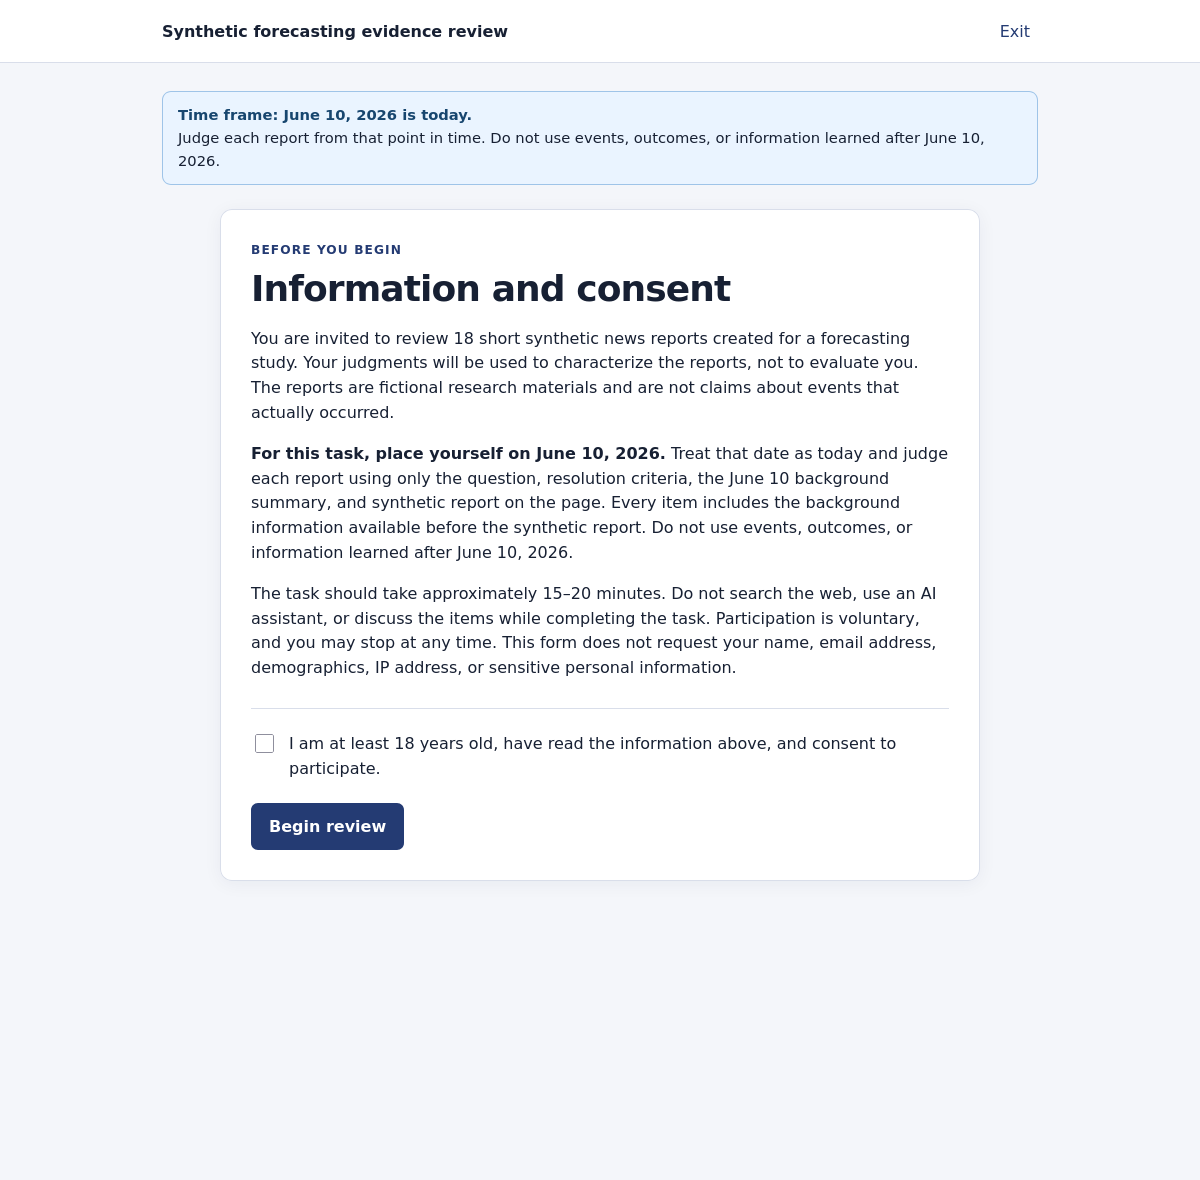
\includegraphics[width=\linewidth]{figures/exp1_stage3_review_consent.png}
  \caption{Information, temporal frame, and consent.}
\end{subfigure}\hfill
\begin{subfigure}[t]{0.60\linewidth}
  \centering
  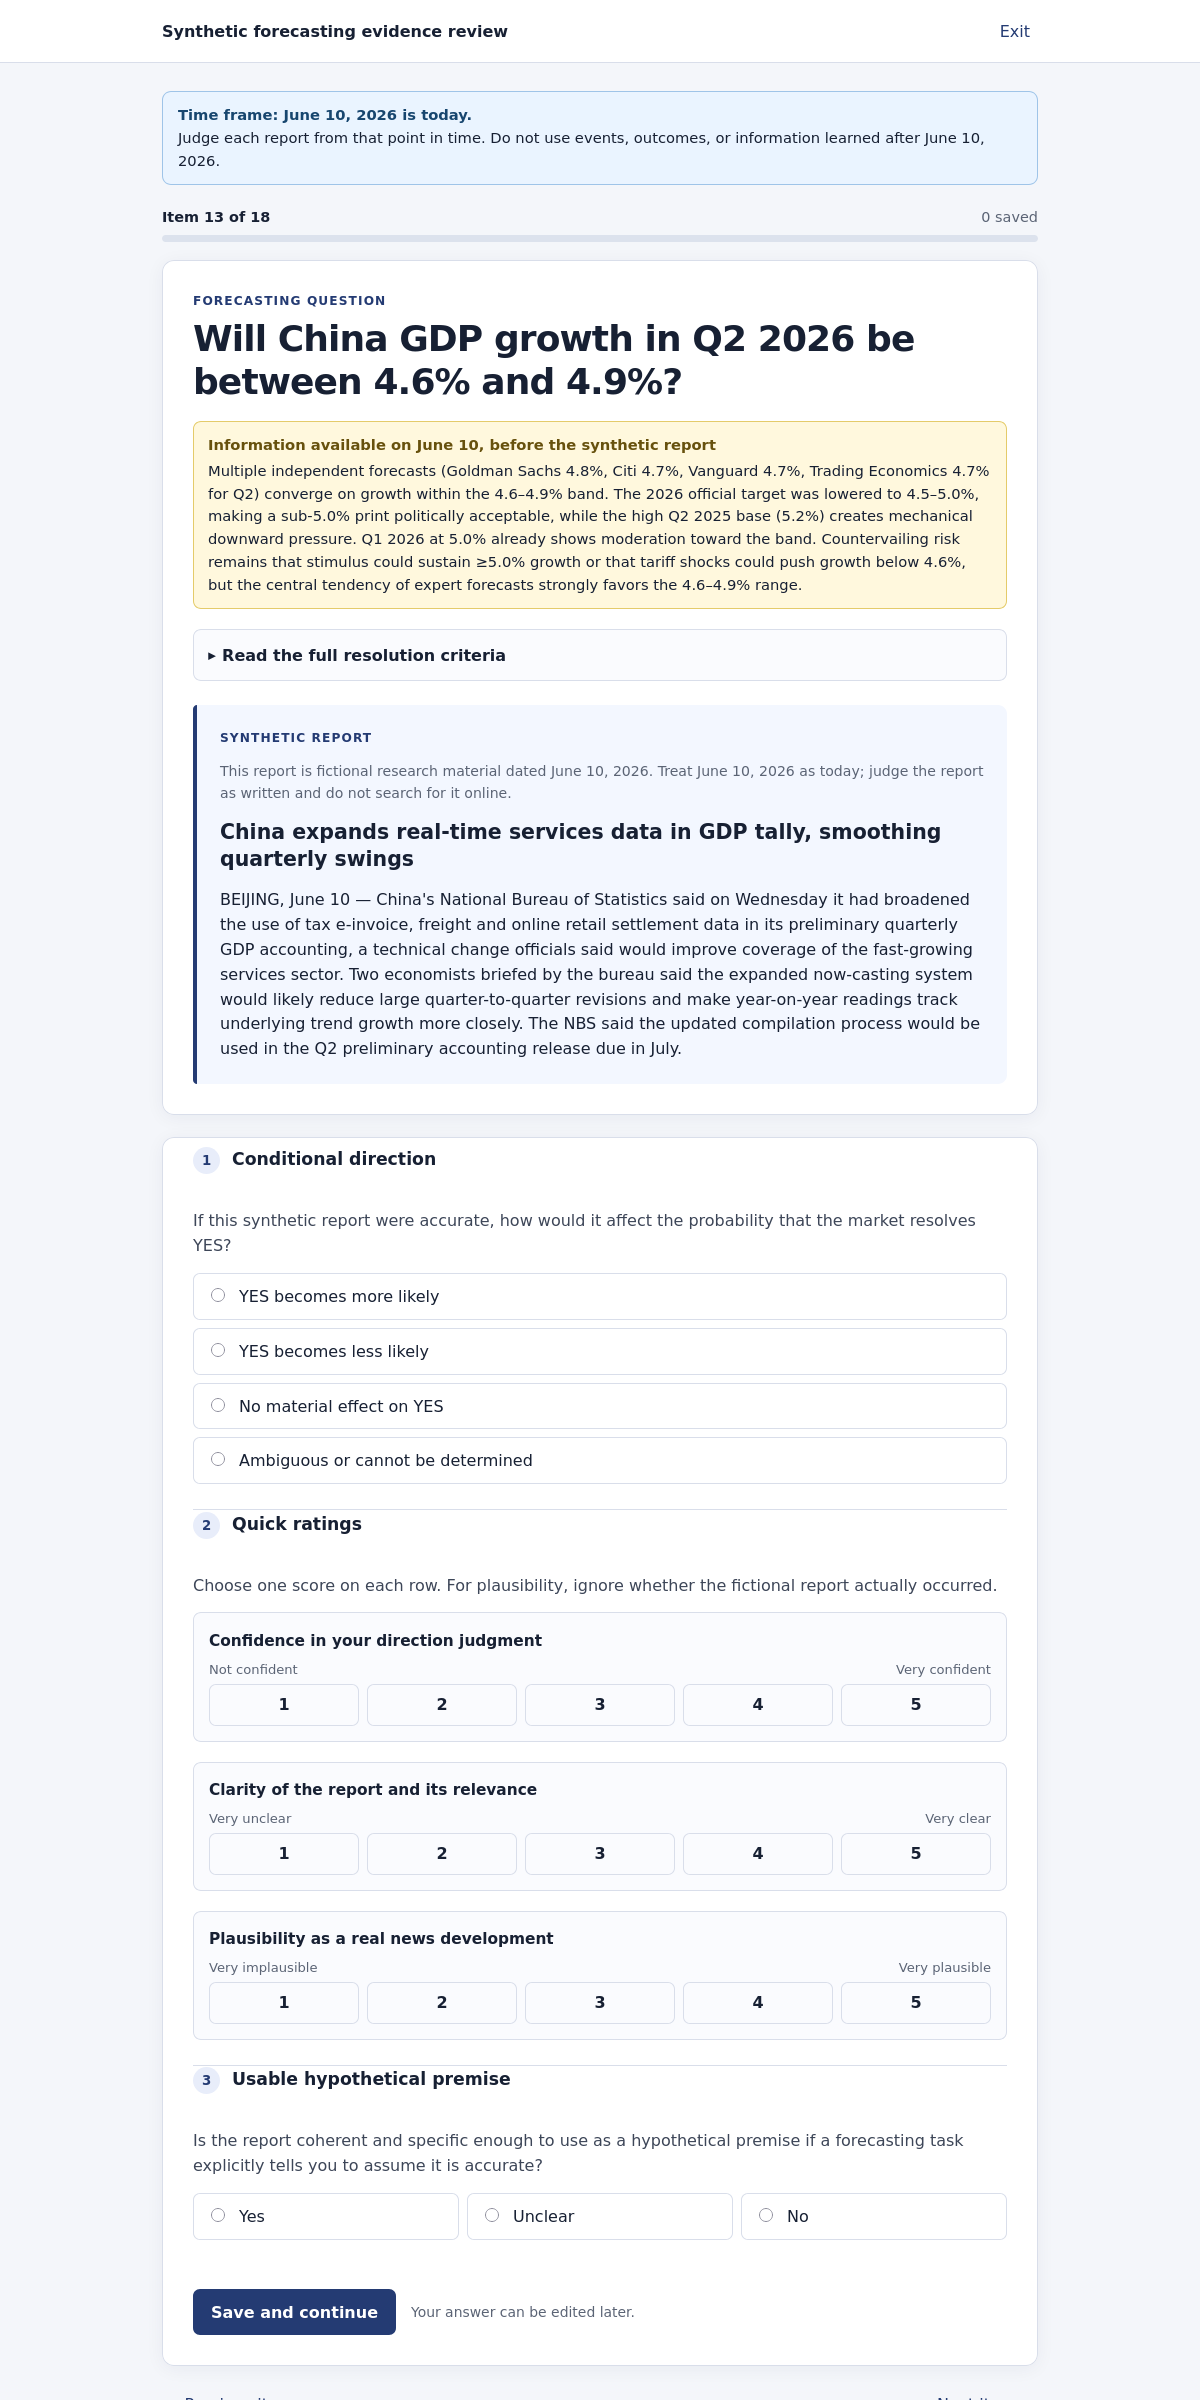
\includegraphics[width=\linewidth]{figures/exp1_stage3_review_item.png}
  \caption{A complete item with June~10 context, synthetic report, and five judgments.}
\end{subfigure}
\caption{\textbf{Stage~3 materials-review interface.} Reviewers enter a private
code before seeing the information-and-consent screen. Each item repeats the
June~10 temporal frame, presents the question and pre-report background, labels
the fictional evidence as a synthetic report, and collects conditional
direction, confidence, clarity, plausibility, and premise usability. Item order
was independently randomized by reviewer. Intended direction and private packet
metadata are hidden.}
\label{fig:exp1-review-interface}
\end{figure}

Orthogonal packets are a useful outcome-relevance control, but are not equivalent
to receiving no new text. A literal no-information update condition would separate
generic prompt-induced revision from response to topically adjacent content.  The very
small hosted-system orthogonal revisions (0.5--1.4~pp) do not substitute for
that control.

\subsubsection{Prompt, retrieval, and runtime confounding}
Agents shared a substantive task contract, while execution was not byte-identical. Hosted
models used Azure Foundry search, while local models used Tavily results in an
Ollama workflow; temperatures and provider behavior also differ. Hosted--local
gaps therefore combine model capability with retrieval and runtime differences.

\subsubsection{Scale, missingness, and dependence}
Realized repeat counts are uneven because failures and top-ups differ by provider.
Equal-weight market aggregation prevents high-coverage markets from dominating
EHC, HFC, and ICS. Movement and sensitivity intervals use 20,000
market-clustered bootstrap draws that retain every packet and repeated initial-run
update from each selected market. The mixed-scale Qwen~2.5-7B row described in
Section~\ref{app:record-processing} remains an appendix compliance diagnostic and is
excluded from the main magnitude comparison.

\subsubsection{Premise acceptance at Stage~3}
Search is intentionally unavailable during updating, and agents are told to
accept the synthetic headline as true. This design measures conditional premise
use rather than source verification or epistemic refusal. The human materials review
uses the same instruction and therefore assesses comprehension and premise
usability. These results do not establish whether a model should trust or verify
the synthetic report.

\subsection{Reproducibility and artifact map}
\label{app:fig-code}

The paper treats the June~17 model-update report and the August~23 final
materials-review summary as the frozen numerical authorities. The relevant
artifacts are:

\begin{itemize}
  \item \textbf{Sampling:}
        \path{exp1_prospective/fetch_markets/select_markets.py} and the June~9
        selection/diversity JSON and manifests in
        \path{exp1_prospective/data/selected_markets/}.
  \item \textbf{Initial elicitation:}
        \path{exp1_prospective/agent/forecast_agent.py} for hosted runs and
        \path{exp1_prospective/agent/run_local_forecast.py} for Ollama runs, with
        records and manifests in \path{exp1_prospective/data/initial_forecasts/}.
  \item \textbf{Interventions:}
        \path{exp1_prospective/agent/build_counterfactuals.py} and the frozen
        \path{exp1_prospective/data/counterfactuals/counterfactuals_2026-06-10.jsonl}.
  \item \textbf{Updates:}
        hosted and local update runners under \path{exp1_prospective/agent/}, with
        update records in \path{exp1_prospective/data/updated_forecasts/}.
  \item \textbf{Evaluation:}
        \path{exp1_prospective/agent/evaluate_consistency.py} and
        \path{exp1_prospective/data/results/consistency_report_2026-06-17.json};
        \path{exp1_prospective/agent/evaluate_clustered_uncertainty.py}
        reconstructs the 20,000-draw market-clustered intervals in
        \path{exp1_prospective/data/results/clustered_movement_uncertainty.json};
        \path{exp1_prospective/agent/audit_orthogonal_abstention.py} writes the
        abstention/magnitude decomposition of Table~\ref{tab:exp1-abstention} to
        \path{exp1_prospective/data/results/orthogonal_abstention.json} and its
        table source, under the same resampling scheme.
  \item \textbf{Human materials review:}
        the frozen protocol, blinded packet, browser application, and tests in
        \path{exp1_prospective/stage3_materials_annotation/};
        \path{make_final_summary.py} reconstructs
        \path{data/exports/final_summary_current.json}, while
        \path{data/exports/agreement_current.json} is the paper-facing agreement
        export.
  \item \textbf{Figures:}
        \path{paper/generate_figures.py} writes the direction-selective panel;
        \path{paper/generate_paper_figures.py} writes the combined
        EHC/sensitivity panel.
\end{itemize}

The model-update tables are defined by the June~17 frozen JSON. The mutable collection
directories contain later records, so evaluating their present contents would
define a different dataset. Bit-for-bit reconstruction begins from the frozen
JSON; a full pipeline reconstruction uses only the manifests and records included
in that freeze.

% ============================================================
% EXPERIMENT 2 -- COIN CITY FULL DETAILS
% ============================================================

\section{Experiment 2: Contextual Relationship Selection and Revision in Coin City}
\label{app:coin-city}

Experiment~2 tests whether context
selects which response relationship a model applies and whether direct target
observations revise that selection. The six primary deployments and symbol-control
comparisons reuse the same 250 seeded episodes, so prompt-arm differences are
paired rather than comparisons between independently sampled tests.

\subsection{Design, Data-Generating Process, and Freeze}
\label{app:coin-city-design}

\subsubsection{Design summary}
The frozen design identifier is
\path{coin_city_stable_relationship_claude_n250_v4}. It contains 250 independent
episodes generated from seeds 930000--930249, five target-city prefixes
\(k\in\{0,1,2,3,4\}\), and three semantic-selection arms frozen before the initial
model calls. Cue-inversion and arbitrary-symbol modules reuse those episode
identities and numerical inputs; each has its own task manifest frozen before its
calls (Section~\ref{app:coin-city-execution}). Every model received the same
episode records, queries, and arm-specific prompt text.

\subsubsection{Balanced latent regimes}
Each episode crosses two binary factors: whether City A or City B is the strongly
responsive reference city, and whether target City C is strongly or weakly
responsive. The closest-balanced allocation contains 63 A-strong/C-strong,
62 A-strong/C-weak, 62 B-strong/C-strong, and 63 B-strong/C-weak episodes.
Within an episode, each city receives an independently sampled stable slope
\[
  g_{ec}\sim
  \begin{cases}
    \mathcal N(0.90,0.03^2), & \text{strong regime},\\
    \mathcal N(0.25,0.03^2), & \text{weak regime}.
  \end{cases}
\]
Thus the cue identifies a response regime but not the realized coefficient.

\subsubsection{Observed cases and forecast query}
Every city has four reference cases arranged as two matched pairs. Rows in a pair
share a starting poll and news magnitude but have opposite signs; the first sign is
random. For reference row \(r\),
\[
  p^{\mathrm{end}}_{ecr}
    = \operatorname{round}_{0.1}
      \left(p^{\mathrm{start}}_{ecr}+g_{ec}x_{ecr}
      +\epsilon_{ecr}\right),
  \qquad \epsilon_{ecr}\sim\mathcal N(0,5^2).
\]
Starting polls are uniform on \([35,65]\), and reference-news magnitudes are drawn
from \(\{6,7,8,9,10\}\). The query shock is drawn from
\(\{-10,\ldots,-4,4,\ldots,10\}\). Its scoring target is the latent conditional
expectation \(p_0+g_Cx\), with no additional query-time observation noise.

The prefix \(k\) exposes the first \(k\) City C rows in their frozen order.
Consequently, \(k=2\) completes the first matched pair and \(k=4\) completes both;
\(k=1\) and \(k=3\) deliberately expose partial pairs. City A and B always
contribute all four rows in the ABC arms.

\begin{center}
\begin{minipage}{\linewidth}
\centering
\captionof{table}{Frozen Coin City design and evaluation dimensions. Final analytic
record counts retain one record per task cell; raw transport-level calls are
discussed in Section~\ref{app:coin-city-limitations}.}
\label{tab:coin-city-design}
\small
\begin{tabular}{p{0.31\linewidth} p{0.62\linewidth}}
\toprule
Quantity & Frozen value \\
\midrule
Independent episodes & 250 \\
Factorial cells & 63, 62, 62, 63 across the four A/B-by-C regimes \\
Target-city prefixes & \(k\in\{0,1,2,3,4\}\) \\
Primary prompt arms & target only; ABC/no C context; ABC/correct C context \\
Intervention modules & ABC/misleading C context; ABC/episode-randomized arbitrary labels \\
Primary deployment roster & Claude Opus~4.8; GPT-5.6; DeepSeek-V4-Pro; Kimi K3; Gemini 3.6 Flash; Claude Opus~5 \\
Symbol-comparison roster & Qwen3 4B/8B/14B/32B; Qwen2.5 7B/14B/32B/72B;
Llama~3.1 8B/70B; DeepSeek-V4-Pro; Kimi K3; Claude Opus~4.8/5; GPT-5.6 Sol \\
Primary task cells / final records & 22,500 / 22,500 (22,497 parseable) \\
Misleading task cells / final records & 7,500 / 7,500 (all parseable) \\
Symbol-comparison task cells / response records & 56,250 / 56,250 (15 models) \\
Strong / weak slope means & 0.90 / 0.25 poll points per news point \\
Slope standard deviation & 0.03 within each regime \\
Reference-case noise & 5 poll points \\
Reference cases per city & 4 (two matched pairs) \\
\bottomrule
\end{tabular}
\end{minipage}
\end{center}

\subsubsection{Freeze and preflight validation}
The GPT-5.6, DeepSeek-V4-Pro, Kimi K3, Gemini 3.6 Flash, and Claude Opus~5
replications reuse the exact task files and prompt hashes created for the original
Claude Opus~4.8 evaluation; no episode was regenerated. Before model calls, the
manifest hashed the engine, task files, answer and scoring keys, validator, runner,
renderer, and launcher. Automated validation confirmed the intended dimensions and
factorial balance, prompt contracts and hashes, correct cue-to-regime mapping,
visible matched pairs, and benchmark reconstruction. No model response or
performance statistic was used by this preflight validator.

\subsection{Prompt Arms and Information Available}
\label{app:coin-city-arms}

\subsubsection{Shared task instructions}
All prompts state that rows are separate polling cases rather than a time series,
positive news favors the candidate, poll change is end minus start, and
within-city responsiveness is stable even though individual polls are noisy. Rows
sharing a pair label are described as having the same starting poll and
equal-magnitude, opposite-sign news. Every displayed row includes the starting
poll, news value, change, and ending poll.

The required answer is a JSON object with exactly a one-sentence
\texttt{rationale} and a numeric \texttt{predicted\_poll} between 0 and 100. The
prompt asks for no step-by-step derivation.

\subsubsection{Five information conditions}
\begin{description}
  \item[Target only.]
  The model sees the first \(k\) City C cases and is explicitly told that no
  additional background information is available. This arm measures recovery
  from target-city evidence alone.

  \item[ABC, no City C context.]
  The model also sees four cases from each reference city, each introduced by a
  background sentence. The strongly responsive reference city is described
  verbatim as receiving ``national news coverage, where campaign stories receive
  sustained attention and tend to produce larger immediate poll movements'', and
  the weakly responsive city as receiving ``local news coverage, where campaign
  stories compete with local issues and tend to produce smaller immediate poll
  movements''. The direction of the coverage-to-response mapping is therefore
  stated in words, though no numerical value is. City C receives no background
  description. This arm tests numeric transfer without a cue that aligns C to
  either reference regime.

  \item[ABC plus correct City C context.]
  The numeric rows and query are identical to the preceding arm. The sole added
  information is that City C receives national or local coverage, correctly
  aligned with its latent strong or weak regime. This is the primary cue-transfer
  condition.

  \item[ABC plus misleading City C context.]
  This intervention arm is identical to the correct-context prompt except that its
  City C sentence names the opposite coverage regime. Every number, case row,
  query, and other instruction is unchanged. This arm tests whether the model
  follows the semantic cue when it conflicts with the truth.

  \item[ABC plus an arbitrary City C label.]
  Every national/local description is replaced by one of two arbitrary labels,
  \texttt{KIV} or \texttt{ZOR}. The prompt states only that cities sharing a label
  share a typical response regime and that the labels have no inherent meaning or
  ordering. Their higher/lower-response mapping reverses on alternating episodes;
  City A and B's numerical cases are therefore the only evidence from which the
  episode-local mapping can be induced before applying City C's label.
\end{description}

No prompt contains a fitted coefficient, an estimator, the strong or weak
numerical means, the case-noise scale, a rule for pooling cities, or any analyst
benchmark. The correct-versus-no-context contrast therefore isolates the one City
C background sentence while holding all displayed numeric evidence fixed; the
correct-versus-misleading comparison isolates the sentence's regime assignment.
The symbol-versus-no-context contrast asks whether the same assignment can be
induced without lexical knowledge of national and local coverage.

Because the reference sentences state the direction of the mapping, the semantic
arms are not by themselves a test of whether that direction can be induced. A
policy that reads no displayed number and assigns slope $1.0$ to the
nationally covered regime and $0.2$ to the locally covered one attains $k=0$
forecast MAE $0.523$ and implied-slope correlation $.996$, better than any
deployment and better than the analogical-regression benchmark of
Table~\ref{tab:coin-city-analogical}; $42$ of $108$ prior pairs on the grid
$\{0.4,\dots,1.5\}\times\{0.0,\dots,0.8\}$ beat every deployment's $k=0$ MAE.
The semantic arms therefore measure how a stated regime assignment is converted
into a numerical response. Two separate controls carry the induction claim: the
arbitrary-symbol arm, whose labels have no stated direction and whose mapping
reverses across episodes, and the reference-selection analysis of
Section~\ref{app:coin-city-reference-selection}, which shows that the forecast
tracks the named reference city's own sampling error rather than any fixed prior.

\subsection{Model Execution and Response Processing}
\label{app:coin-city-execution}

\subsubsection{Deployment configurations}
Table~\ref{tab:coin-city-execution} reports the effective API settings used for
production. Temperature refers to the value sent to the provider: GPT-5.6 and
Claude Opus~5 omit it even though the local GPT run manifest records a default of
zero. No deployment used tools or retrieval.

\begin{center}
\begin{minipage}{\linewidth}
\centering
\captionof{table}{Production deployment configuration and primary-arm parse counts.}
\label{tab:coin-city-execution}
\scriptsize
\setlength{\tabcolsep}{3.5pt}
\begin{tabular}{p{0.16\linewidth} p{0.21\linewidth} p{0.27\linewidth} @{\hspace{1.5em}} r r}
\toprule
Deployment & Interface & Reasoning / sampling & Output ceiling & Parsed \\
\midrule
Claude Opus~4.8 & Anthropic Messages via Azure & temperature 0 & 512 & 3,750 \\
GPT-5.6 & OpenAI Responses & low reasoning; temperature omitted & 4,096 & 3,749 \\
DeepSeek-V4-Pro & OpenAI Chat Completions & temperature 0 & 4,096 & 3,750 \\
Kimi K3 & OpenAI Chat Completions & low reasoning; temperature 0 & 16,384 & 3,750 \\
Gemini 3.6 Flash & Gemini OpenAI-compatible Chat & low reasoning; temperature 0 & 16,384 & 3,750 \\
Claude Opus~5 & Foundry Anthropic Messages & default extended thinking; temperature omitted & 4,096 & 3,748 \\
\bottomrule
\end{tabular}
\end{minipage}
\end{center}

Claude Opus~5 returns extended thinking before its answer; the runner therefore
selects its first text block. Gemini is the sole fast-tier deployment, so the six
systems should be read as a replication set rather than a tier-matched leaderboard.
Authentication material was supplied at runtime and was not written to source,
manifests, logs, or response files.

\subsubsection{Deployment attempts, retries, and pilots}
Every primary model--prompt pair received one application-level attempt. A failed
or answerless task was not re-asked. HTTP-client retries were disabled for GPT,
DeepSeek, Kimi, and Opus~5. The original Opus~4.8 client allowed up to two
transport retries. Gemini's runner allowed adaptive pre-model transport retries
but recorded none in the completed shards. These transport policies do not alter
the one-answer-per-task analytic rule.

Before production, 119 Kimi, 15 Gemini, and 17 Opus~5 task-shaped calls were used
only to select configurations that reliably returned the required JSON schema.
Forecast accuracy was not inspected. The calls are archived separately and are
excluded from every denominator and analysis; each production namespace began
empty. Production tasks were sharded only for throughput.

\subsubsection{Response parsing and record selection}
The parser scans the raw reply for JSON objects, retains the last object with an
exact \texttt{predicted\_poll} key whose value converts to a number in
\([0,100]\), truncates the retained rationale to 500 characters, and stores at
most 8,000 raw characters. When duplicate task records exist, the analysis keeps
the latest parseable response, allowing a valid response to supersede an earlier
error. A single offline normalization removed whitespace from JSON keys in one
otherwise valid Opus~4.8 reply; this recovered one primary record without another
model call. Other record-level corrections are documented in
Section~\ref{app:coin-city-limitations}.

\subsubsection{Misleading-context design}
The cue-inversion module begins from the frozen semantic-selection tasks. Before
any inversion call, its builder verifies that every prompt equals its
correct-context counterpart under
exactly one sentence substitution and that all numeric content is unchanged. The
cue is inverted for all 1,250 episode-prefix tasks: 625 strong-city tasks are
described as weak and 625 weak-city tasks as strong. Each deployment uses the
same client and production configuration as its correct-context arm.

\subsubsection{Arbitrary-symbol design}
The symbol builder generates 1,250 matched prompts from the same frozen
episodes and verifies that their complete sequence of numeric tokens is identical
to the correct-context arm. The higher-response label is \texttt{KIV} in 125
episodes and \texttt{ZOR} in 125; the target regime-by-label cells contain 62--63
episodes each. A prompt validator rejects national/local and strong/weak semantic
descriptions. At \(k=0\), City C supplies no numerical cases, so its correct regime
can be recovered only by decoding the label from City A and B's examples.

For DeepSeek-V4-Pro, we collected all 1,250 symbol tasks and contemporaneously
re-collected all 2,500 no-context and semantic-context tasks on the same reachable
Azure resource, using one deployment identifier and configuration. The released
15-model comparison combines that triplet with Qwen3-4B, Qwen3-8B,
Qwen3-14B, Qwen3-32B, Qwen2.5-7B, Qwen2.5-14B, Qwen2.5-32B, Qwen2.5-72B,
Llama~3.1-8B, Llama~3.1-70B, Kimi K3, Claude Opus~4.8, Claude Opus~5, and
GPT-5.6 Sol.

The eight Qwen and two Llama checkpoints received all 3,750 prompts through vLLM
in bfloat16, with temperature-zero decoding, a 3,072-token model context, and a
512-token output ceiling. Qwen uses the no-thinking chat template; Llama uses its
native instruction template. Qwen2.5-14B uses two-way and Qwen3-32B and
Qwen2.5-32B four-way tensor parallelism, while Qwen2.5-72B and Llama~3.1-70B use
eight-way tensor parallelism.

For Kimi K3, Claude Opus~5, and GPT-5.6 Sol, the comparison reuses each
deployment's preserved no-context and semantic-context responses and adds only
the 1,250 symbol prompts under the same model-specific production protocol.
Claude Opus~4.8's symbol arm instead ran on a second Azure resource serving the
same deployment and used a 1,024-token rather than 512-token ceiling; all 1,250
responses returned valid JSON. We therefore treat its arm contrast as a
cross-run robustness result and do not use it to rank providers.

Every runner verifies the frozen task hash before generation and writes a
timestamped manifest. Each released model has 1,250 unique response records in
every arm; this count does not imply that every prediction parsed. No primary
response file or frozen task is overwritten. Original outputs are preserved, and
the final tables use matched complete cases after the no-call arithmetic reparse
described in Section~\ref{app:coin-city-limitations}.

\subsection{Estimands, Benchmarks, and Statistical Inference}
\label{app:coin-city-analysis}

\subsubsection{Forecast and latent-response estimands}
Forecast error is measured against the latent conditional expectation rather than
a newly sampled noisy ending poll:
\[
  \operatorname{MAE}
  =\frac{1}{n}\sum_{e=1}^{n}
    \left|\widehat p_e-(p_{0e}+g_{Ce}x_e)\right|.
\]
For every nonzero query shock, a forecast also identifies an implied slope
\(\widehat g_e=(\widehat p_e-p_{0e})/x_e\). We report its mean absolute error from
\(g_{Ce}\) and its Pearson correlation with \(g_{Ce}\) across episodes.
Correlation is needed because a nearly constant prior-mean slope can attain
moderate MAE while failing to distinguish strong from weak cities.

Within each deployment and prefix, the three primary-arm metrics use the common
intersection of episodes with parseable responses in all three arms. Arm
contrasts are paired by episode and prefix. The misleading-arm table uses its
final unique parseable record for every task. The arbitrary-symbol analysis uses
each model's corresponding common intersection across its three matched arms.

\subsubsection{Analyst-only benchmarks}
The ABC OLS benchmark fits poll change on news through the origin using every
displayed A, B, and available C row. The target-only OLS benchmark uses only
displayed City C rows and is undefined at \(k=0\). Both are reconstructed from
the visible data by the analyst; neither the estimator nor its output appears in
a model prompt.

The label-conditioned analogical regression implements the minimal structured
inductive policy defined in Methods. It
fits separate through-origin slopes to City A and City B, uses City C's coverage
label to select the reference assigned to the same response regime, and predicts
with that slope. At $k>0$, it pools the selected reference rows with the visible
City C rows before refitting. In the misleading arm, the inverted label selects
the opposite reference. The implementation uses only displayed rows; neither the
estimator nor its output appears in a model prompt.
\begin{center}
\begin{minipage}{\linewidth}
\centering
\captionof{table}{Zero-shot behavior of the analogical policy and the six model
deployments. At $k=0$, City C has no numerical cases. Model columns give the
range across deployments; forecast MAE is in poll points.}
\label{tab:coin-city-analogical}
\small
\begin{tabular}{l r r c c}
\toprule
Cue & Policy MAE & Policy $\rho$ & Model MAE range & Model $\rho$ range \\
\midrule
Correct & 1.842 & .656 & 1.596--2.474 & [.52,\,.70] \\
Inverted & 4.561 & $-.667$ & 4.204--4.361 & [$-.68$,\,$-.50$] \\
\bottomrule
\end{tabular}
\end{minipage}
\end{center}


\subsubsection{Uncertainty and comparison families}
Primary arm contrasts use percentile intervals from 2,000 bootstrap resamples of
the paired episode-level absolute-error difference. Deterministic, model-specific
seeds make these intervals reproducible. The \(k=0\) pairwise model table uses
4,000 paired bootstrap resamples with seed 20260812 and the common episode
intersection for each model pair. Negative differences favor the first-listed
condition or model.

The episodes are the resampling units. Intervals are pointwise descriptions of
this fixed seeded synthetic evaluation: they are not simultaneous bands across
prefixes, and no multiple-comparison correction is applied. Accordingly, the
number of pairwise intervals excluding zero is not used as an estimand; each
interval supports only its displayed cell.

\subsection{Response-Inference Diagnostics}
\label{app:coin-city-results}

The tables below retain a common arm and prefix ordering. Within a deployment and
prefix, all three primary arms use the same complete-case episode set; \(n\) is
repeated so that every exception is visible. Boldface identifies the lowest
forecast MAE or slope MAE, and the highest slope correlation, within that
deployment and prefix.

\subsubsection{Per-deployment primary-arm recovery}

\begingroup
\setlength{\topsep}{3pt}
\setlength{\partopsep}{0pt}
\setlength{\parsep}{0pt}
\setlength{\itemsep}{0pt}
\begin{center}
\begin{minipage}{\linewidth}
\centering
\captionof{table}{Claude Opus~4.8 forecast and latent-response diagnostics for every prompt
arm. Forecast MAE is in poll points; slope MAE and $\rho$ compare the implied
response with the true City C slope.}
\label{tab:coin-city-recovery}
\small
\begin{tabular}{c l r r r r}
\toprule
$k$ & Arm & $n$ & Forecast MAE & Slope MAE & $\rho(\hat g,g_C)$ \\
\midrule
0 & Target only & 250 & 2.321 & .332 & .019 \\
  & ABC, no C context & 250 & 2.651 & .379 & -.063 \\
  & ABC + C context & 250 & \textbf{1.817} & \textbf{.265} & \textbf{.700} \\
\midrule
1 & Target only & 250 & 3.730 & .549 & .371 \\
  & ABC, no C context & 250 & 2.438 & .358 & .322 \\
  & ABC + C context & 250 & \textbf{2.147} & \textbf{.316} & \textbf{.584} \\
\midrule
2 & Target only & 250 & 2.668 & .403 & .383 \\
  & ABC, no C context & 250 & \textbf{2.041} & \textbf{.296} & \textbf{.492} \\
  & ABC + C context & 250 & 2.079 & .308 & .491 \\
\midrule
3 & Target only & 250 & 2.485 & .358 & .449 \\
  & ABC, no C context & 250 & 2.128 & .305 & .513 \\
  & ABC + C context & 250 & \textbf{1.977} & \textbf{.291} & \textbf{.627} \\
\midrule
4 & Target only & 250 & 2.209 & .324 & .498 \\
  & ABC, no C context & 250 & 1.929 & .281 & .542 \\
  & ABC + C context & 250 & \textbf{1.760} & \textbf{.257} & \textbf{.658} \\
\bottomrule
\end{tabular}
\end{minipage}
\end{center}

\begin{center}
\begin{minipage}{\linewidth}
\centering
\captionof{table}{GPT-5.6 forecast and latent-response diagnostics on the same frozen
prompts. Metrics use episodes parseable in all three arms at each prefix.}
\label{tab:coin-city-recovery-gpt56}
\small
\begin{tabular}{c l r r r r}
\toprule
$k$ & Arm & $n$ & Forecast MAE & Slope MAE & $\rho(\hat g,g_C)$ \\
\midrule
0 & Target only & 250 & 3.596 & .511 & .054 \\
  & ABC, no C context & 250 & 2.518 & .352 & -.041 \\
  & ABC + C context & 250 & \textbf{1.596} & \textbf{.224} & \textbf{.678} \\
\midrule
1 & Target only & 249 & 2.993 & .439 & .394 \\
  & ABC, no C context & 249 & 2.768 & .399 & .302 \\
  & ABC + C context & 249 & \textbf{1.586} & \textbf{.225} & \textbf{.669} \\
\midrule
2 & Target only & 250 & 2.560 & .387 & .459 \\
  & ABC, no C context & 250 & 2.050 & .299 & .534 \\
  & ABC + C context & 250 & \textbf{1.854} & \textbf{.268} & \textbf{.606} \\
\midrule
3 & Target only & 250 & 2.240 & .328 & .528 \\
  & ABC, no C context & 250 & 1.967 & .286 & .584 \\
  & ABC + C context & 250 & \textbf{1.773} & \textbf{.256} & \textbf{.600} \\
\midrule
4 & Target only & 250 & 2.153 & .318 & .577 \\
  & ABC, no C context & 250 & 1.746 & .253 & .653 \\
  & ABC + C context & 250 & \textbf{1.594} & \textbf{.228} & \textbf{.664} \\
\bottomrule
\end{tabular}
\end{minipage}
\end{center}

\begin{center}
\begin{minipage}{\linewidth}
\centering
\captionof{table}{DeepSeek-V4-Pro forecast and latent-response diagnostics on the same
frozen prompts. All 250 episodes parsed in every arm and prefix.}
\label{tab:coin-city-recovery-deepseek}
\small
\begin{tabular}{c l r r r r}
\toprule
$k$ & Arm & $n$ & Forecast MAE & Slope MAE & $\rho(\hat g,g_C)$ \\
\midrule
0 & Target only & 250 & \textbf{2.447} & .353 & -.027 \\
  & ABC, no C context & 250 & 2.841 & .401 & -.027 \\
  & ABC + C context & 250 & 2.474 & \textbf{.344} & \textbf{.523} \\
\midrule
1 & Target only & 250 & 3.585 & .525 & .334 \\
  & ABC, no C context & 250 & 3.130 & .458 & .302 \\
  & ABC + C context & 250 & \textbf{2.456} & \textbf{.347} & \textbf{.578} \\
\midrule
2 & Target only & 250 & 3.380 & .501 & .319 \\
  & ABC, no C context & 250 & 3.423 & .502 & .365 \\
  & ABC + C context & 250 & \textbf{2.687} & \textbf{.391} & \textbf{.492} \\
\midrule
3 & Target only & 250 & 2.908 & .424 & .454 \\
  & ABC, no C context & 250 & 3.224 & .463 & .403 \\
  & ABC + C context & 250 & \textbf{2.797} & \textbf{.403} & \textbf{.504} \\
\midrule
4 & Target only & 250 & 2.812 & .415 & .430 \\
  & ABC, no C context & 250 & 3.040 & .459 & .366 \\
  & ABC + C context & 250 & \textbf{2.809} & \textbf{.409} & \textbf{.470} \\
\bottomrule
\end{tabular}
\end{minipage}
\end{center}

\begin{center}
\begin{minipage}{\linewidth}
\centering
\captionof{table}{Kimi K3 forecast and latent-response diagnostics on the same frozen
prompts. All 250 episodes parsed in every arm and prefix.}
\label{tab:coin-city-recovery-kimi}
\small
\begin{tabular}{c l r r r r}
\toprule
$k$ & Arm & $n$ & Forecast MAE & Slope MAE & $\rho(\hat g,g_C)$ \\
\midrule
0 & Target only & 250 & 3.352 & .476 & -.016 \\
  & ABC, no C context & 250 & 2.548 & .357 & -.021 \\
  & ABC + C context & 250 & \textbf{1.886} & \textbf{.266} & \textbf{.593} \\
\midrule
1 & Target only & 250 & 3.362 & .494 & .365 \\
  & ABC, no C context & 250 & 3.370 & .490 & .345 \\
  & ABC + C context & 250 & \textbf{2.382} & \textbf{.341} & \textbf{.579} \\
\midrule
2 & Target only & 250 & 3.194 & .491 & .387 \\
  & ABC, no C context & 250 & 3.114 & .487 & .352 \\
  & ABC + C context & 250 & \textbf{2.306} & \textbf{.349} & \textbf{.455} \\
\midrule
3 & Target only & 250 & 2.816 & .412 & .430 \\
  & ABC, no C context & 250 & 2.636 & .407 & .410 \\
  & ABC + C context & 250 & \textbf{2.005} & \textbf{.292} & \textbf{.609} \\
\midrule
4 & Target only & 250 & 2.378 & .357 & .444 \\
  & ABC, no C context & 250 & 1.957 & .284 & \textbf{.622} \\
  & ABC + C context & 250 & \textbf{1.840} & \textbf{.263} & .601 \\
\bottomrule
\end{tabular}
\end{minipage}
\end{center}


\begin{center}
\begin{minipage}{\linewidth}
\centering
\captionof{table}{Gemini 3.6 Flash forecast and latent-response diagnostics on the same
frozen prompts. All 250 episodes parsed in every arm and prefix.}
\label{tab:coin-city-recovery-gemini}
\small
\begin{tabular}{c l r r r r}
\toprule
$k$ & Arm & $n$ & Forecast MAE & Slope MAE & $\rho(\hat g,g_C)$ \\
\midrule
0 & Target only & 250 & 2.534 & .370 & .002 \\
  & ABC, no C context & 250 & 2.552 & .356 & .078 \\
  & ABC + C context & 250 & \textbf{2.174} & \textbf{.302} & \textbf{.559} \\
\midrule
1 & Target only & 250 & 3.733 & .550 & \textbf{.403} \\
  & ABC, no C context & 250 & 3.717 & .548 & .361 \\
  & ABC + C context & 250 & \textbf{3.300} & \textbf{.500} & .292 \\
\midrule
2 & Target only & 250 & \textbf{3.564} & \textbf{.558} & \textbf{.348} \\
  & ABC, no C context & 250 & 3.703 & .579 & .335 \\
  & ABC + C context & 250 & 3.600 & .569 & .330 \\
\midrule
3 & Target only & 250 & 3.370 & .513 & .314 \\
  & ABC, no C context & 250 & 3.092 & .460 & .397 \\
  & ABC + C context & 250 & \textbf{3.047} & \textbf{.443} & \textbf{.471} \\
\midrule
4 & Target only & 250 & 3.308 & .498 & .389 \\
  & ABC, no C context & 250 & 2.911 & .447 & .433 \\
  & ABC + C context & 250 & \textbf{2.793} & \textbf{.419} & \textbf{.447} \\
\bottomrule
\end{tabular}
\end{minipage}
\end{center}


\begin{center}
\begin{minipage}{\linewidth}
\centering
\captionof{table}{Claude Opus~5 forecast and latent-response diagnostics on the same
frozen prompts. Two responses exhausted the output budget on extended thinking and
returned no answer, one in each ABC arm.}
\label{tab:coin-city-recovery-opus5}
\small
\begin{tabular}{c l r r r r}
\toprule
$k$ & Arm & $n$ & Forecast MAE & Slope MAE & $\rho(\hat g,g_C)$ \\
\midrule
0 & Target only & 250 & 2.359 & .333 & -.018 \\
  & ABC, no C context & 250 & 2.619 & .371 & -.007 \\
  & ABC + C context & 250 & \textbf{1.764} & \textbf{.247} & \textbf{.617} \\
\midrule
1 & Target only & 249 & 3.549 & .520 & .391 \\
  & ABC, no C context & 249 & 2.303 & .338 & .370 \\
  & ABC + C context & 249 & \textbf{1.741} & \textbf{.254} & \textbf{.601} \\
\midrule
2 & Target only & 250 & 3.804 & .596 & .309 \\
  & ABC, no C context & 250 & 2.680 & .412 & .389 \\
  & ABC + C context & 250 & \textbf{2.060} & \textbf{.314} & \textbf{.524} \\
\midrule
3 & Target only & 250 & 3.022 & .461 & .379 \\
  & ABC, no C context & 250 & 2.363 & .356 & .459 \\
  & ABC + C context & 250 & \textbf{2.075} & \textbf{.309} & \textbf{.550} \\
\midrule
4 & Target only & 249 & 2.700 & .418 & .443 \\
  & ABC, no C context & 249 & 2.369 & .366 & .459 \\
  & ABC + C context & 249 & \textbf{2.201} & \textbf{.335} & \textbf{.499} \\
\bottomrule
\end{tabular}
\end{minipage}
\end{center}




\subsubsection{Misleading-cue results}

\begin{center}
\begin{minipage}{\linewidth}
\centering
\captionof{table}{Misleading-cue arm: forecast MAE and latent-slope correlation at each
City C prefix. The prompt is byte-identical to the correct-context arm except that the
City C sentence names the opposite response regime. Negative $\rho$ means the implied
response is anti-correlated with the truth, i.e. the deployment has adopted the stated
regime. Each of the six deployments contributes all 1,250 prompts.}
\label{tab:coin-city-wrong-context}
\small
\setlength{\tabcolsep}{4pt}
\begin{tabular}{l rr rr rr rr rr}
\toprule
& \multicolumn{2}{c}{$k{=}0$} & \multicolumn{2}{c}{$k{=}1$} & \multicolumn{2}{c}{$k{=}2$}
& \multicolumn{2}{c}{$k{=}3$} & \multicolumn{2}{c}{$k{=}4$} \\
\cmidrule(lr){2-3}\cmidrule(lr){4-5}\cmidrule(lr){6-7}\cmidrule(lr){8-9}\cmidrule(lr){10-11}
Model & MAE & $\rho$ & MAE & $\rho$ & MAE & $\rho$ & MAE & $\rho$ & MAE & $\rho$ \\
\midrule
Claude Opus~4.8 & 4.20 & $-.66$ & 3.88 & $-.51$ & 3.04 & $.09$ & 2.61 & $.22$ & 2.31 & $.34$ \\
GPT-5.6 & 4.23 & $-.68$ & 4.15 & $-.63$ & 2.78 & $.17$ & 2.71 & $.25$ & 2.10 & $.46$ \\
DeepSeek-V4-Pro & 4.36 & $-.62$ & 4.46 & $-.48$ & 3.61 & $.07$ & 3.39 & $.14$ & 3.04 & $.32$ \\
Kimi K3 & 4.31 & $-.62$ & 4.12 & $-.25$ & 3.03 & $.15$ & 2.72 & $.14$ & 2.18 & $.44$ \\
Gemini 3.6 Flash & 4.29 & $-.50$ & 4.40 & $-.06$ & 3.93 & $.24$ & 3.52 & $.25$ & 2.93 & $.36$ \\
Claude Opus~5 & 4.25 & $-.62$ & 3.15 & $-.21$ & 2.59 & $.27$ & 2.41 & $.41$ & 2.36 & $.47$ \\
\bottomrule
\end{tabular}
\end{minipage}
\end{center}

\subsubsection{Arbitrary-symbol induction results}
\label{app:coin-city-symbol-context}

\begin{center}
\begin{minipage}{\linewidth}
\centering
\captionof{table}{\textbf{Fifteen-system episode-randomized arbitrary-symbol
comparison at $k=0$.} Panel A reports forecast calibration; Panel B reports
response-regime discrimination. All arms share the frozen numeric task content;
Section~\ref{app:coin-city-execution} documents model-specific execution and the
Opus~4.8 cross-resource deviation. MAE is in poll points;
$\rho$ correlates implied and true latent slopes; Acc. classifies the response
regime at slope 0.575. Each $\Delta$ is symbol minus no context, with a paired
95\% episode-bootstrap interval. With no City C examples, its label can be decoded
only from City A/B examples.}
\label{tab:coin-city-symbol-context}
\scriptsize
\setlength{\tabcolsep}{2.2pt}
% Generated by paper/generate_coin_city_symbol_context_tables.py from the final 2026-08-24 comparison artifact; do not edit.
\textit{Panel A: Forecast accuracy}\par\vspace{-2pt}
\resizebox{0.82\linewidth}{!}{%
\begin{tabular}{l r rrr c}
\toprule
Model & $n$ & No context & Semantic & Symbol & $\Delta$MAE [95\% CI] \\
\midrule
Qwen3-4B & 250 & 2.896 & 2.365 & 2.892 & $-.005$ $[-.088,.074]$ \\
Qwen2.5-7B & 250 & 2.911 & 2.669 & 3.248 & $+.338$ $[.027,.682]$ \\
Qwen3-8B & 250 & 2.985 & 2.859 & 2.973 & $-.011$ $[-.239,.207]$ \\
Qwen2.5-14B & 250 & 2.606 & 2.548 & 2.711 & $+.105$ $[-.178,.388]$ \\
Qwen3-14B & 250 & 2.632 & 2.241 & 2.812 & $+.180$ $[-.188,.548]$ \\
Qwen3-32B & 250 & 2.482 & 2.069 & 2.914 & $+.432$ $[.119,.752]$ \\
Qwen2.5-32B & 250 & 2.679 & 2.404 & 3.208 & $+.529$ $[.169,.924]$ \\
Qwen2.5-72B & 250 & 2.474 & 2.383 & 3.398 & $+.924$ $[.582,1.310]$ \\
\midrule
Llama-3.1-8B & 242 & 3.113 & 3.386 & 3.605 & $+.492$ $[.029,.980]$ \\
Llama-3.1-70B & 250 & 3.483 & 3.761 & 3.931 & $+.448$ $[.030,.886]$ \\
DeepSeek V4-Pro & 250 & 2.622 & 2.588 & 2.729 & $+.107$ $[-.222,.452]$ \\
Kimi K3 & 250 & 2.548 & 1.886 & 2.051 & $-.497$ $[-.765,-.211]$ \\
Claude Opus~4.8 & 250 & 2.651 & 1.817 & 2.067 & $-.584$ $[-.858,-.314]$ \\
Claude Opus~5 & 250 & 2.619 & 1.764 & 2.017 & $-.603$ $[-.869,-.336]$ \\
GPT-5.6 & 250 & 2.518 & 1.596 & 1.744 & $-.774$ $[-1.011,-.533]$ \\
\bottomrule
\end{tabular}}
\par\vspace{4pt}
\textit{Panel B: Response-regime discrimination}\par\vspace{-2pt}
\resizebox{\linewidth}{!}{%
\begin{tabular}{l r rr c rr c}
\toprule
& & \multicolumn{2}{c}{$\rho(\hat g,g_C)$} & & \multicolumn{2}{c}{Regime accuracy} & \\
\cmidrule(lr){3-4}\cmidrule(lr){6-7}
Model & $n$ & No context & Symbol & $\Delta\rho$ [95\% CI] & No context & Symbol & $\Delta$Acc. [95\% CI] \\
\midrule
Qwen3-4B & 250 & -.011 & .085 & $+.095$ $[-.060,.230]$ & .496 & .512 & $+.016$ $[-.008,.044]$ \\
Qwen2.5-7B & 250 & -.034 & .230 & $+.264$ $[.112,.406]$ & .500 & .572 & $+.072$ $[.020,.128]$ \\
Qwen3-8B & 250 & -.014 & .009 & $+.023$ $[-.128,.171]$ & .492 & .516 & $+.024$ $[-.012,.060]$ \\
Qwen2.5-14B & 250 & -.029 & .208 & $+.236$ $[.107,.356]$ & .492 & .580 & $+.088$ $[.020,.152]$ \\
Qwen3-14B & 250 & -.057 & .342 & $+.398$ $[.253,.541]$ & .496 & .660 & $+.164$ $[.088,.240]$ \\
Qwen3-32B & 250 & .075 & .377 & $+.302$ $[.177,.433]$ & .524 & .656 & $+.132$ $[.060,.200]$ \\
Qwen2.5-32B & 250 & -.015 & .358 & $+.372$ $[.226,.502]$ & .500 & .648 & $+.148$ $[.088,.208]$ \\
Qwen2.5-72B & 250 & .027 & .408 & $+.381$ $[.250,.508]$ & .516 & .632 & $+.116$ $[.056,.176]$ \\
\midrule
Llama-3.1-8B & 242 & -.042 & .003 & $+.045$ $[-.123,.250]$ & .467 & .512 & $+.045$ $[-.029,.120]$ \\
Llama-3.1-70B & 250 & -.039 & .385 & $+.424$ $[.314,.543]$ & .500 & .592 & $+.092$ $[.036,.152]$ \\
DeepSeek V4-Pro & 250 & .018 & .454 & $+.436$ $[.323,.558]$ & .520 & .692 & $+.172$ $[.104,.240]$ \\
Kimi K3 & 250 & -.021 & .612 & $+.633$ $[.520,.742]$ & .468 & .804 & $+.336$ $[.272,.400]$ \\
Claude Opus~4.8 & 250 & -.063 & .560 & $+.623$ $[.492,.744]$ & .448 & .760 & $+.312$ $[.240,.380]$ \\
Claude Opus~5 & 250 & -.007 & .583 & $+.591$ $[.485,.697]$ & .496 & .780 & $+.284$ $[.220,.348]$ \\
GPT-5.6 & 250 & -.041 & .655 & $+.696$ $[.597,.807]$ & .464 & .836 & $+.372$ $[.312,.432]$ \\
\bottomrule
\end{tabular}}

\end{minipage}
\end{center}

\begin{center}
\begin{minipage}{\linewidth}
\centering
\captionof{table}{\textbf{Matched open-weight scaling across target-city
observations.} Symbol-minus-no-context effects are reported for Qwen2.5
32B/72B and Llama~3.1 8B/70B at each City C prefix. Negative
$\Delta$MAE favors the induced symbol mapping; positive $\Delta\rho$ and
$\Delta$accuracy indicate better regime discrimination.}
\label{tab:coin-city-symbol-scaling}
\scriptsize
\setlength{\tabcolsep}{2.2pt}
\resizebox{\linewidth}{!}{% Generated by paper/generate_coin_city_symbol_context_tables.py from the final 2026-08-24 comparison artifact; do not edit.
\begin{tabular}{l rr ccc}
\toprule
Model & $k$ & $n$ & $\Delta$MAE [95\% CI] & $\Delta\rho$ [95\% CI] & $\Delta$Acc. [95\% CI] \\
\midrule
Qwen2.5-32B & 0 & 250 & $+.529$ $[.169,.924]$ & $+.372$ $[.226,.502]$ & $+.148$ $[.088,.208]$ \\
 & 1 & 250 & $+.124$ $[-.188,.441]$ & $+.096$ $[.010,.190]$ & $+.068$ $[.016,.124]$ \\
 & 2 & 250 & $+.184$ $[-.044,.421]$ & $-.010$ $[-.059,.037]$ & $-.012$ $[-.048,.024]$ \\
 & 3 & 250 & $+.462$ $[.222,.710]$ & $-.033$ $[-.096,.024]$ & $-.004$ $[-.044,.036]$ \\
 & 4 & 250 & $+.255$ $[-.001,.524]$ & $-.010$ $[-.059,.033]$ & $-.016$ $[-.048,.016]$ \\
\midrule
Qwen2.5-72B & 0 & 250 & $+.924$ $[.582,1.310]$ & $+.381$ $[.250,.508]$ & $+.116$ $[.056,.176]$ \\
 & 1 & 250 & $+.189$ $[-.148,.520]$ & $+.166$ $[.075,.265]$ & $+.076$ $[.024,.128]$ \\
 & 2 & 250 & $-.024$ $[-.286,.239]$ & $+.070$ $[.017,.127]$ & $+.016$ $[-.028,.060]$ \\
 & 3 & 250 & $+.252$ $[-.050,.549]$ & $+.019$ $[-.051,.092]$ & $+.024$ $[-.024,.068]$ \\
 & 4 & 250 & $+.019$ $[-.280,.322]$ & $+.011$ $[-.067,.088]$ & $+.020$ $[-.024,.064]$ \\
\midrule
Llama-3.1-8B & 0 & 242 & $+.492$ $[.029,.980]$ & $+.045$ $[-.123,.250]$ & $+.045$ $[-.029,.120]$ \\
 & 1 & 240 & $-2.318$ $[-3.256,-1.373]$ & $+.120$ $[-.022,.263]$ & $-.050$ $[-.129,.029]$ \\
 & 2 & 238 & $-2.454$ $[-3.433,-1.529]$ & $+.106$ $[-.038,.260]$ & $-.017$ $[-.097,.055]$ \\
 & 3 & 244 & $-.867$ $[-1.739,.085]$ & $-.088$ $[-.238,.061]$ & $-.078$ $[-.156,.000]$ \\
 & 4 & 246 & $-1.396$ $[-2.321,-.489]$ & $+.100$ $[-.067,.245]$ & $-.049$ $[-.122,.024]$ \\
\midrule
Llama-3.1-70B & 0 & 250 & $+.448$ $[.030,.886]$ & $+.424$ $[.314,.543]$ & $+.092$ $[.036,.152]$ \\
 & 1 & 250 & $+.194$ $[-.245,.658]$ & $+.077$ $[-.026,.190]$ & $-.016$ $[-.076,.040]$ \\
 & 2 & 250 & $-.200$ $[-.548,.149]$ & $+.039$ $[-.026,.106]$ & $-.016$ $[-.068,.036]$ \\
 & 3 & 250 & $-.345$ $[-.621,-.075]$ & $+.037$ $[-.015,.087]$ & $+.020$ $[-.016,.056]$ \\
 & 4 & 250 & $-.079$ $[-.306,.158]$ & $+.034$ $[-.006,.082]$ & $+.012$ $[-.020,.048]$ \\
\bottomrule
\end{tabular}
}
\end{minipage}
\end{center}

At $k=0$, Qwen3 provides a within-family contrast.
Symbol-minus-no-context $\Delta\rho$ is $.095$ $[-.060,.230]$ at 4B and $.023$
$[-.128,.171]$ at 8B, but $.398$ $[.253,.541]$ at 14B and $.302$ $[.177,.433]$
at 32B; the regime-accuracy contrasts follow the same pattern. The 4B and 8B
intervals span zero, whereas the 14B and 32B intervals do not. The 32B point
estimate sits below the 14B one, so this is a boundary among the tested Qwen3
checkpoints rather than a monotone or universal parameter threshold. The smaller checkpoints are not wholesale task
failures: their semantic-context slopes correlate $.370$ and $.286$ with truth,
versus $-.011$ and $-.014$ without context.

All four tested Qwen2.5 checkpoints discriminate under arbitrary labels
($\Delta\rho=.264/.236/.372/.381$ at 7B/14B/32B/72B), reinforcing the family
qualification. Their symbol-minus-no-context MAE changes are
$+.338/+.105/+.529/+.924$: mapping discrimination does not ensure calibrated
numerical use. Direct City C examples
make the large-Qwen symbol advantage redundant; by $k=3$--4, the 32B and 72B
$\Delta\rho$ and $\Delta$accuracy intervals span zero.

Llama~3.1 provides a second within-family contrast: $\Delta\rho=.045$
$[-.123,.250]$ at 8B and $.424$ $[.314,.543]$ at 70B. The 70B
regime-accuracy contrast is $.092$ $[.036,.152]$, although its MAE rises by
$.448$ $[.030,.886]$. In Qwen3 the mapping-recovery interval excludes zero only
from 14B upward, and in Llama only at 70B. The positive Qwen2.5-7B and
Qwen2.5-14B estimates, despite Qwen3-8B's interval spanning zero, indicate that
the tested transition depends on model family rather than parameter count. Mapping recovery and numerical calibration remain
separate outcomes.

DeepSeek improves discrimination ($\Delta\rho=.436$ $[.323,.558]$) without a
detectable zero-shot MAE change. Kimi, both Opus deployments, and GPT combine
mapping recovery with lower forecast error: their $\Delta\rho$ values are
$.633/.623/.591/.696$, while MAE falls by $.497/.584/.603/.774$ points.
Cross-provider magnitudes remain descriptive because runtimes, reasoning settings,
and output ceilings differ.

\subsubsection{Paired cue effects and interpretation}

\begin{center}
\begin{minipage}{\linewidth}
\centering
\captionof{table}{Paired forecast-MAE difference between the correct-context arm
and the context-blind ABC OLS benchmark, which the analyst fits through the origin
on every displayed A, B and available City C row. Negative values favour the
deployment. Boldface marks intervals excluding zero.}
\label{tab:coin-city-vs-ols}
\small
\setlength{\tabcolsep}{5pt}
\begin{tabular}{l ccccc}
\toprule
Model & $k{=}0$ & $k{=}1$ & $k{=}2$ & $k{=}3$ & $k{=}4$ \\
\midrule
Claude Opus~4.8 & \textbf{$-.73$} & $-.18$ & $-.05$ & $-.01$ & $-.08$ \\
GPT-5.6 & \textbf{$-.95$} & \textbf{$-.74$} & \textbf{$-.28$} & $-.21$ & \textbf{$-.24$} \\
DeepSeek-V4-Pro & $-.07$ & $.13$ & \textbf{$.56$} & \textbf{$.81$} & \textbf{$.97$} \\
Kimi K3 & \textbf{$-.66$} & $.06$ & $.18$ & $.02$ & $.01$ \\
Gemini 3.6 Flash & \textbf{$-.37$} & \textbf{$.98$} & \textbf{$1.47$} & \textbf{$1.06$} & \textbf{$.96$} \\
Claude Opus~5 & \textbf{$-.78$} & \textbf{$-.57$} & $-.07$ & $.09$ & \textbf{$.36$} \\
\bottomrule
\end{tabular}
\end{minipage}
\end{center}
\endgroup

At $k=0$ every deployment matches or beats the context-blind benchmark, and five
of the six intervals exclude zero: with no City C cases, the only way to separate
City C from the pooled A/B fit is to use its description. The advantage does not
persist once City C supplies its own rows. By $k=2$ DeepSeek-V4-Pro and Gemini 3.6
Flash are significantly worse than the benchmark, Claude Opus~5 becomes so at
$k=4$, and the remaining deployments are indistinguishable from it. The cue effect
this experiment measures is therefore a zero-shot phenomenon, and a plain
through-origin estimator remains competitive once direct target evidence
accumulates.

In the zero-shot matched-reference comparison, the target-city description changes
the influence of the A/B cases on forecasts. All six $k=0$ bootstrap intervals
exclude zero. A label-conditioned benchmark that selects a reference, estimates
its slope, and transfers that estimate reproduces the aggregate pattern; the
comparison does not identify the model's internal algorithm.
More target rows do not monotonically reduce error: DeepSeek and Opus~5 drift by
$0.34$ and $0.44$ points from $k=0$ to $k=4$, and Gemini's context advantage is
significant only at $k\in\{0,1\}$. Short, noisy prefixes can temporarily mislead
either arm.

\subsection{Does the Forecast Track the Cue-Named Reference?}
\label{app:coin-city-reference-selection}

Two accounts explain the correct-versus-no-context contrast equally well. Under a
lexical-prior account the model maps the City C coverage sentence straight to a
remembered response magnitude and never reads City A or City B's numbers. Under a
reference-selection account it uses the cue to choose a reference city, estimates
that city's slope from its four displayed cases, and transfers the estimate. Both
predict a regime-level correlation, because the cue and the latent regime coincide.

The design separates them. A through-origin fit to four noisy reference cases has
a within-regime standard deviation of $.332$ against a generator standard
deviation of $.03$, so the matched reference's fitted slope correlates only $.656$
with the true City C slope where the regime indicator correlates $.996$. That
sampling error is the discriminating signal: a forecaster that is deterministic
given the cue cannot reproduce it, whereas one that transfers a fitted reference
slope inherits it. For every deployment, arm and prefix we therefore report
\[
  r\!\left(\widehat g_e,\;\widehat\beta^{\mathrm{ref}}_e \;\middle|\; R_e\right),
\]
the partial correlation between the forecast-implied slope and a reference city's
through-origin OLS slope, controlling for the response regime $R_e$ that the City
C label names. Arms with no City C label are scored against the true regime and
report the regime-matched and regime-mismatched reference instead. Intervals are
2,000-draw episode bootstraps with deterministic per-cell seeds, and the analysis
makes no model call.

\begin{center}
\begin{minipage}{\linewidth}
\centering
\captionof{table}{Partial correlation between the forecast-implied City C slope and
each reference city's fitted slope at $k=0$, controlling for the regime the City C
label names. ``Named'' is the reference the label points to, or the regime-matched
reference in the two arms without a label. Boldface marks named-reference intervals
excluding zero.}
\label{tab:coin-city-reference-selection}
\small
\setlength{\tabcolsep}{4pt}
% Generated by paper/generate_coin_city_reference_selection_tables.py from analysis/reference_selection_results.json; do not edit.
\begin{tabular}{l cc cc cc cc}
\toprule
& \multicolumn{2}{c}{Target only} & \multicolumn{2}{c}{ABC, no label}
& \multicolumn{2}{c}{ABC + correct} & \multicolumn{2}{c}{ABC + inverted} \\
\cmidrule(lr){2-3}\cmidrule(lr){4-5}\cmidrule(lr){6-7}\cmidrule(lr){8-9}
Model & Named & Other & Named & Other & Named & Other & Named & Other \\
\midrule
Claude Opus~4.8 & $-.08$ & $-.02$ & \textbf{$.39$} & $.53$ & \textbf{$.62$} & $.07$ & \textbf{$.71$} & $.04$ \\
GPT-5.6 & \textbf{$.15$} & $-.03$ & \textbf{$.67$} & $.68$ & \textbf{$.86$} & $.04$ & \textbf{$.90$} & $.03$ \\
DeepSeek V4-Pro & $.00$ & $.01$ & \textbf{$.40$} & $.42$ & \textbf{$.51$} & $.05$ & \textbf{$.61$} & $.06$ \\
Kimi K3 & $-.01$ & $.04$ & \textbf{$.55$} & $.60$ & \textbf{$.71$} & $.10$ & \textbf{$.64$} & $.06$ \\
Gemini 3.6 Flash & $-.09$ & $-.07$ & \textbf{$.42$} & $.44$ & \textbf{$.69$} & $.09$ & \textbf{$.63$} & $.05$ \\
Claude Opus~5 & $-.07$ & $-.00$ & \textbf{$.52$} & $.53$ & \textbf{$.78$} & $.07$ & \textbf{$.75$} & $.05$ \\
\bottomrule
\end{tabular}

\end{minipage}
\end{center}

The four arms make four different predictions and all four hold. With no reference
cases displayed at all, the target-only arm loads on neither reference: eleven of
its twelve intervals span zero. With both references displayed but no City C label,
every deployment loads on the two references almost equally, the pooling signature
of a model that cannot tell which reference applies. Adding the correct label
concentrates the loading on the named reference and removes it from the other,
every ``other'' interval spanning zero. Inverting the label moves the loading
wholesale onto the reference that the false cue names, leaving the truth-matched
reference near zero.

The forecast therefore tracks the particular reference city the label names,
including that city's sampling error, whether or not the label is correct. No
prior attached to the words \emph{national} and \emph{local} reproduces this. It
also explains why implied-slope correlations plateau near $.66$ rather than near
$.996$: faithful transfer of a noisy reference estimate is capped at that
reference's own $.656$ correlation with the truth. GPT-5.6 and Claude Opus~4.8
slightly exceed the cap at $k=0$, which is what blending a reference estimate with
a regime prior produces.

\begin{center}
\begin{minipage}{\linewidth}
\centering
\captionof{table}{The same partial correlation in the arbitrary-symbol arm at
$k=0$, where \texttt{KIV} and \texttt{ZOR} carry no stated direction and their
mapping reverses across episodes. The no-label columns repeat each model's pooling
control. Boldface marks symbol named-reference intervals excluding zero.}
\label{tab:coin-city-reference-selection-symbol}
\small
\setlength{\tabcolsep}{4pt}
% Generated by paper/generate_coin_city_reference_selection_tables.py from analysis/reference_selection_results.json; do not edit.
\begin{tabular}{l r cc cc}
\toprule
& & \multicolumn{2}{c}{ABC, no label} & \multicolumn{2}{c}{ABC + symbol} \\
\cmidrule(lr){3-4}\cmidrule(lr){5-6}
Model & $n$ & Named & Other & Named & Other \\
\midrule
Qwen3-4B & 250 & $.05$ & $-.09$ & $.00$ & $-.03$ \\
Qwen2.5-7B & 250 & $.11$ & $.15$ & \textbf{$.28$} & $.10$ \\
Qwen3-8B & 250 & $.12$ & $.06$ & $.09$ & $.11$ \\
Qwen2.5-14B & 250 & $.31$ & $.20$ & \textbf{$.32$} & $.03$ \\
Qwen3-14B & 250 & $.26$ & $.20$ & \textbf{$.46$} & $.06$ \\
Qwen3-32B & 250 & $.20$ & $.19$ & \textbf{$.40$} & $.03$ \\
Qwen2.5-32B & 250 & $.22$ & $.15$ & \textbf{$.38$} & $.02$ \\
Qwen2.5-72B & 250 & $.25$ & $.18$ & \textbf{$.53$} & $.04$ \\
Llama-3.1-8B & 249 & $-.02$ & $.07$ & $-.00$ & $-.08$ \\
Llama-3.1-70B & 250 & $.28$ & $.19$ & \textbf{$.54$} & $.00$ \\
DeepSeek V4-Pro & 250 & $.40$ & $.42$ & \textbf{$.51$} & $.07$ \\
Kimi K3 & 250 & $.55$ & $.60$ & \textbf{$.86$} & $.01$ \\
Claude Opus~4.8 & 250 & $.39$ & $.53$ & \textbf{$.71$} & $-.05$ \\
Claude Opus~5 & 250 & $.52$ & $.53$ & \textbf{$.83$} & $.02$ \\
GPT-5.6 & 250 & $.67$ & $.68$ & \textbf{$.98$} & $.02$ \\
\bottomrule
\end{tabular}

\end{minipage}
\end{center}

Applying the estimator to the arbitrary-symbol arm removes the lexical account
entirely. Twelve of the fifteen released systems have a named-reference interval
excluding zero, and the three that do not---Qwen3-4B, Qwen3-8B and
Llama~3.1-8B---are exactly the three whose symbol-minus-no-context $\Delta\rho$
intervals span zero in Table~\ref{tab:coin-city-symbol-context}. The two
statistics are computed from different quantities and agree on all fifteen
systems.

\subsection{Linear-Probe Analysis of Cue-Conditioned Representations}
\label{app:coin-city-mechanistic-probe}

\subsubsection{Behavioral Screening Criteria}
Before extracting activations for the original scaling comparison, we screened the
same frozen held-out prompts with Qwen3-8B, Qwen3-14B, dense Qwen3-32B, and
Qwen2.5-72B-Instruct. Each checkpoint received 16 test episodes crossed with
$k\in\{0,4\}$ and correct, absent, or inverted City C context (96 prompts), with
96/96 parseable forecasts.

\begin{center}
\begin{minipage}{\linewidth}
\centering
\captionof{table}{\textbf{Behavioral screening results for the linear-probe analysis.}
Entries are paired mean differences with 95\% episode-bootstrap intervals
($n=16$). Evidence is no-context $k=4$ minus $k=0$ aligned slope; selection is
correct minus absent context at $k=0$; reversal is inverted minus correct context
at $k=0$; forecast penalty is inverted minus correct poll MAE at $k=0$. Positive
evidence and selection, negative reversal, and a positive forecast penalty are
the predicted directions.}
\label{tab:coin-city-behavioral-gate}
\scriptsize
\setlength{\tabcolsep}{2.4pt}
\resizebox{\linewidth}{!}{% Generated by paper/generate_coin_city_mechanistic_comparison.py; do not edit.
\begin{tabular}{lcccc}
\toprule
Model & Evidence & Selection & Reversal & Forecast penalty \\
\midrule
Qwen3-8B & $+.119$ $[-.094,+.374]$ & $+.078$ $[-.012,+.219]$ & $-.140$ $[-.315,+.007]$ & $+.812$ $[-.063,+2.023]$ \\
Qwen3-14B & $+.394$ $[+.152,+.734]$ & $+.261$ $[+.134,+.400]$ & $-.380$ $[-.597,-.172]$ & $+1.662$ $[+.252,+3.155]$ \\
Qwen3-32B & $+.315$ $[+.017,+.646]$ & $+.234$ $[+.111,+.407]$ & $-.390$ $[-.554,-.221]$ & $+1.965$ $[+1.013,+3.083]$ \\
Qwen2.5-72B & $+.246$ $[+.001,+.529]$ & $+.096$ $[-.077,+.259]$ & $-.433$ $[-.674,-.220]$ & $+2.206$ $[+.957,+3.620]$ \\
\bottomrule
\end{tabular}
}
\end{minipage}
\end{center}

The 14B and 32B intervals exclude zero in all four predicted directions. For 72B,
the evidence, reversal, and forecast-penalty intervals exclude zero, while the
correct-versus-absent selection interval spans zero. All four 8B intervals span
zero. We use 32B for the dense Qwen3 scaling comparison and 72B for a
cross-generation comparison; neither is interpreted as another point on a
monotonic size curve. This four-model gate was frozen before the
cross-architecture extension. Qwen3-4B and Llama-3.1-8B subsequently reused the
identical task file and sealed split without reopening model, layer, target, or
endpoint selection.

\subsubsection{Frozen Activation and Probe Protocol}
We selected 64 episodes without replacement, balanced over which reference city
was strongly responsive and whether City C's latent regime was strong or weak.
Forty-eight episodes form a development set and 16 form a sealed test set. Each
episode is rendered at $k=0$ and $k=4$ under correct, absent, and inverted context,
giving 384 activation records. Within an episode-prefix pair the three prompts
have identical numeric content. The only intervention is the City C relationship
description.

For the final input token, we save the embedding output and every transformer-block
output. The resulting tensor dimensions are $[384,37,2560]$ for Qwen3-4B;
$[384,37,4096]$ for Qwen3-8B; $[384,33,4096]$ for Llama-3.1-8B;
$[384,41,5120]$ for Qwen3-14B; $[384,65,5120]$ for Qwen3-32B; and
$[384,81,8192]$ for Qwen2.5-72B-Instruct. We fit separate dual-ridge probes at
each layer and $k$, using only correct-context development episodes. Four
cell-balanced development folds select the ridge strength from
$\{10^{-4},3\!\times\!10^{-3},10^{-1},3,100\}$ and then select one reported
layer. The untouched test episodes are evaluated in all three context arms
($n=16$ per arm). A 10,000-repeat held-out label permutation test keeps the
development-selected layer, ridge strength, and fitted probe fixed. Thus neither
the test labels nor test-arm scores select the reported layer.

We probe three increasingly strict targets: the binary strong/weak regime; the
full realized slope $g_C$; and the within-regime residual
$g_C-.90$ for strong episodes or $g_C-.25$ for weak episodes. The residual target
controls for regime membership, which explains nearly all slope variance.
Mean-pooled embedding and final-layer states are additional pooling controls.

\begin{center}
\begin{minipage}{\linewidth}
\centering
\captionof{table}{\textbf{Six-model correct-context probe summary.}
Each entry gives $k=0/k=4$ on the 16 sealed episodes. Layers and ridge strengths
were selected on development episodes only. Residual $p$ is the one-sided
10,000-repeat held-out label-permutation value.}
\label{tab:coin-city-mechanistic-summary}
\small
\setlength{\tabcolsep}{3.0pt}
\resizebox{\linewidth}{!}{% Generated by paper/generate_coin_city_mechanistic_comparison.py; do not edit.
\begin{tabular}{lcccc}
\toprule
Model & Regime AUC & Full-slope $R^2$ & Residual-slope $R^2$ & Residual $p$ \\
\midrule
Qwen3-4B & 1.000/1.000 & .960/.885 & -.389/-.227 & .927/.614 \\
Qwen3-8B & .844/1.000 & .713/.653 & -.359/-.374 & .502/.735 \\
Llama-3.1-8B & 1.000/.984 & .913/.731 & -.126/-.207 & .380/.572 \\
Qwen3-14B & 1.000/.984 & .898/.627 & -.531/-.128 & .315/.450 \\
Qwen3-32B & 1.000/1.000 & .967/.811 & -.269/.003 & .477/.221 \\
Qwen2.5-72B & 1.000/1.000 & .975/.869 & -.451/-.053 & .675/.447 \\
\bottomrule
\end{tabular}
}
\end{minipage}
\end{center}

\begin{center}
\begin{minipage}{\linewidth}
\centering
\captionof{table}{\textbf{Held-out layer-wise open-weight probe.} AUC is reported
for the regime target and $R^2$ for both slope targets. Correct, none, and wrong
score the same development-selected probe against the true City C target under
the three context arms; wrong/cue instead scores the inverted arm against the
relationship named by its cue. $p$ is the one-sided held-out label-permutation
value on the correct-context test episodes.}
\label{tab:coin-city-mechanistic-probe}
\scriptsize
\setlength{\tabcolsep}{2.4pt}
\resizebox{\linewidth}{!}{% Generated by paper/generate_coin_city_mechanistic_comparison.py; do not edit.
\begin{tabular}{lllr rrrrrr}
\toprule
Model & $k$ & Target & Layer & Dev CV & Correct & None & Wrong/true & Wrong/cue & $p$ \\
\midrule
Qwen3-4B & 0 & Regime (AUC) & 1 & 1.000 & 1.000 & .562 & .000 & 1.000 & $<.001$ \\
 &  & Full slope ($R^2$) & 24 & .936 & .960 & -.517 & -2.614 & .956 & $<.001$ \\
 &  & Residual slope ($R^2$) & 15 & .054 & -.389 & -.296 & -.258 & -- & $.927$ \\
\cmidrule(lr){2-10}
 & 4 & Regime (AUC) & 19 & 1.000 & 1.000 & .609 & .094 & .906 & $<.001$ \\
 &  & Full slope ($R^2$) & 20 & .805 & .885 & -.065 & -1.147 & .492 & $<.001$ \\
 &  & Residual slope ($R^2$) & 14 & .004 & -.227 & .089 & -.183 & -- & $.614$ \\
\midrule
Qwen3-8B & 0 & Regime (AUC) & 19 & 1.000 & .844 & .453 & .078 & .922 & $.009$ \\
 &  & Full slope ($R^2$) & 23 & .870 & .713 & -.697 & -2.344 & .771 & $<.001$ \\
 &  & Residual slope ($R^2$) & 1 & .063 & -.359 & -.673 & -.378 & -- & $.502$ \\
\cmidrule(lr){2-10}
 & 4 & Regime (AUC) & 23 & .925 & 1.000 & .578 & .000 & 1.000 & $<.001$ \\
 &  & Full slope ($R^2$) & 23 & .462 & .653 & -.512 & -1.550 & .693 & $<.001$ \\
 &  & Residual slope ($R^2$) & 33 & .030 & -.374 & -1.003 & -.029 & -- & $.735$ \\
\midrule
Llama-3.1-8B & 0 & Regime (AUC) & 1 & 1.000 & 1.000 & .359 & .000 & 1.000 & $<.001$ \\
 &  & Full slope ($R^2$) & 1 & .907 & .913 & -18.953 & -2.629 & .972 & $<.001$ \\
 &  & Residual slope ($R^2$) & 12 & .018 & -.126 & -.458 & -.227 & -- & $.380$ \\
\cmidrule(lr){2-10}
 & 4 & Regime (AUC) & 1 & 1.000 & .984 & .438 & .000 & 1.000 & $<.001$ \\
 &  & Full slope ($R^2$) & 1 & .751 & .731 & -15.450 & -2.082 & .808 & $<.001$ \\
 &  & Residual slope ($R^2$) & 10 & .006 & -.207 & -.148 & -.150 & -- & $.572$ \\
\midrule
Qwen3-14B & 0 & Regime (AUC) & 2 & 1.000 & 1.000 & .422 & .000 & 1.000 & $<.001$ \\
 &  & Full slope ($R^2$) & 26 & .874 & .898 & -.522 & -2.423 & .943 & $<.001$ \\
 &  & Residual slope ($R^2$) & 34 & .159 & -.531 & -9.255 & -.096 & -- & $.315$ \\
\cmidrule(lr){2-10}
 & 4 & Regime (AUC) & 26 & .880 & .984 & .688 & .109 & .891 & $<.001$ \\
 &  & Full slope ($R^2$) & 26 & .408 & .627 & -.411 & -1.191 & .409 & $<.001$ \\
 &  & Residual slope ($R^2$) & 1 & -.013 & -.128 & -.605 & -.159 & -- & $.450$ \\
\midrule
Qwen3-32B & 0 & Regime (AUC) & 27 & 1.000 & 1.000 & .359 & .000 & 1.000 & $<.001$ \\
 &  & Full slope ($R^2$) & 47 & .930 & .967 & -.027 & -2.570 & .958 & $<.001$ \\
 &  & Residual slope ($R^2$) & 1 & .062 & -.269 & -.232 & -.259 & -- & $.477$ \\
\cmidrule(lr){2-10}
 & 4 & Regime (AUC) & 44 & 1.000 & 1.000 & .562 & .000 & 1.000 & $<.001$ \\
 &  & Full slope ($R^2$) & 47 & .797 & .811 & -.160 & -1.694 & .666 & $<.001$ \\
 &  & Residual slope ($R^2$) & 1 & .043 & .003 & .062 & -.000 & -- & $.221$ \\
\midrule
Qwen2.5-72B & 0 & Regime (AUC) & 53 & 1.000 & 1.000 & .469 & .000 & 1.000 & $<.001$ \\
 &  & Full slope ($R^2$) & 58 & .955 & .975 & -1.050 & -2.958 & .969 & $<.001$ \\
 &  & Residual slope ($R^2$) & 32 & .061 & -.451 & -1.192 & -.401 & -- & $.675$ \\
\cmidrule(lr){2-10}
 & 4 & Regime (AUC) & 58 & .995 & 1.000 & .922 & .062 & .938 & $<.001$ \\
 &  & Full slope ($R^2$) & 58 & .678 & .869 & -.468 & -1.072 & .493 & $<.001$ \\
 &  & Residual slope ($R^2$) & 1 & -.017 & -.053 & -.063 & -.053 & -- & $.447$ \\
\bottomrule
\end{tabular}
}
\end{minipage}
\end{center}

\begin{figure}[ht]
  \centering
  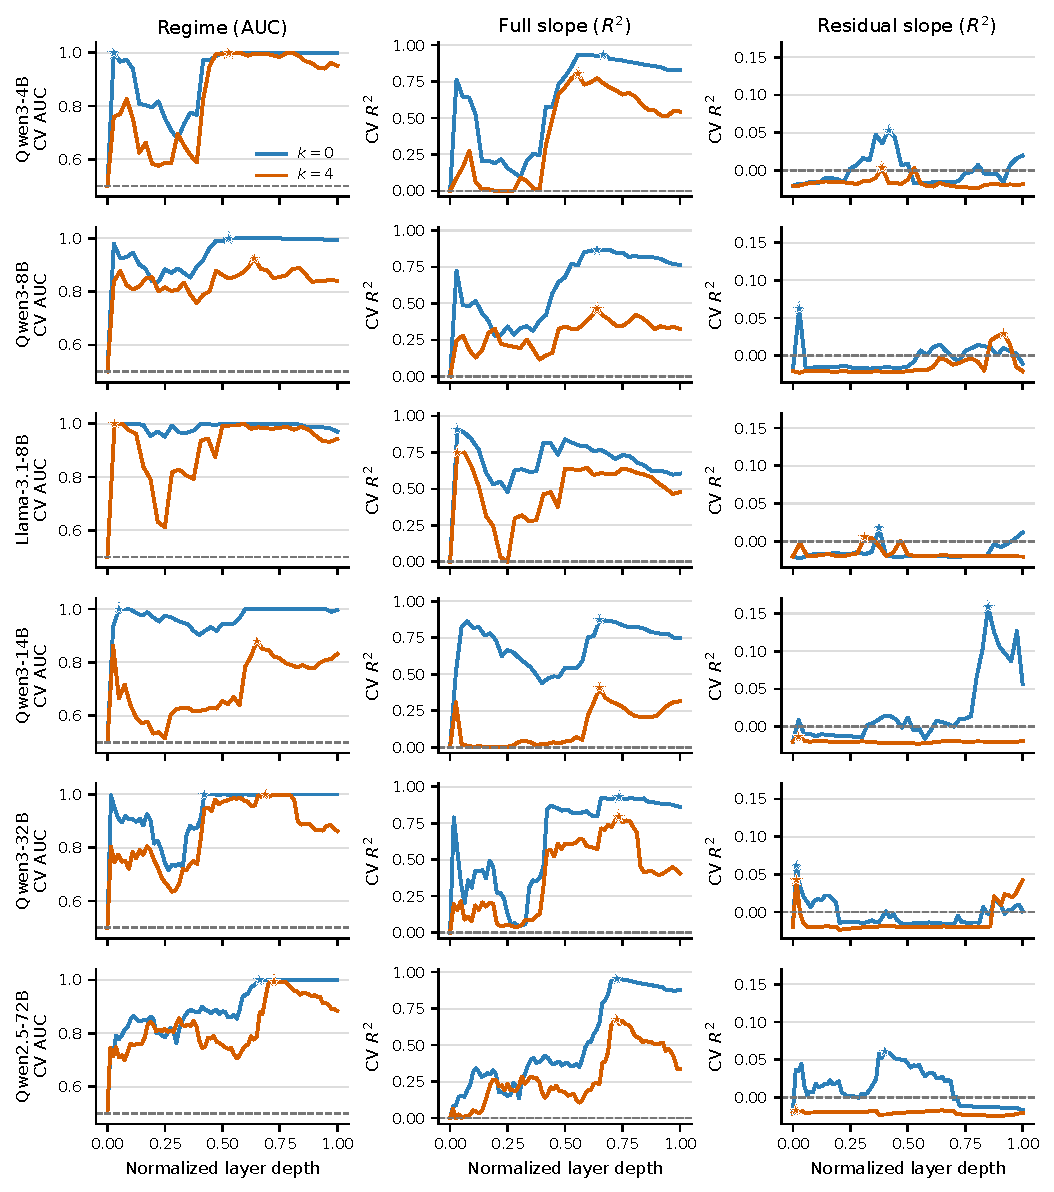
\includegraphics[width=\linewidth]{figures/exp2_qwen3_mechanistic_probe.pdf}
  \caption{\textbf{Development layer trajectories for the six-model probe.}
  Curves show four-fold development CV rather than test performance; stars mark
  the layer selected before the test set was opened. Layer depth is normalized
  because the checkpoints have 32--80 transformer blocks. The regime and
  full-slope signals are broad, whereas residual-slope CV is weak and does not
  survive held-out evaluation.}
  \label{fig:coin-city-mechanistic-probe}
\end{figure}

\subsubsection{Regime and Full-Slope Decodability}
Across the six checkpoints and two evidence depths, correct-context regime AUC
is $.844$--$1.000$ and full-slope $R^2$ is $.627$--$.975$
(Table~\ref{tab:coin-city-mechanistic-summary}). This information is not a
context-invariant encoding of the true coefficient: removing the City C
description drives selected-layer full-slope $R^2$ below zero in all 12
model--$k$ cells. Under inversion, true-target regime AUC falls to
$.000$--$.109$ while cue-target AUC is $.891$--$1.000$; the full-slope probe
likewise fits the cue-assigned relationship better than the true one. The Llama
replication shows that this pattern is not specific to the Qwen checkpoints.
Across both model families, the linearly available signal therefore tracks the
response family that context assigns to City C.

\subsubsection{Specificity: Within-Regime Residuals}
The probes do not detect episode-specific variation within a response family.
The 12 correct-context residual-slope $R^2$ values range from $-.531$ to $.003$,
and none of their permutation tests rejects the null ($p=.221$--$.927$); 33 of
36 arm-level residual scores are nonpositive. Mean-pooled input embeddings for
every Qwen checkpoint already give perfect regime AUC and full-slope
$R^2=.988$--$.993$ under correct context because the explicit description
identifies a regime and the regime means dominate slope variance. Llama input
embeddings likewise give perfect regime AUC and full-slope
$R^2=.756/.827$. Every input-embedding residual-slope score is negative.
The layer-wise result is therefore evidence that the cue-selected response
family is linearly represented, not evidence that the exact continuous $g_C$ is
recovered. The original behavioral inversion screen connects this representation
to output sensitivity in the three larger screened checkpoints: inverted context
raises $k=0$ forecast MAE by $1.66$, $1.96$, and $2.21$ points for 14B, 32B, and
72B, respectively.

\subsubsection{Power-Matched Semantic and Arbitrary-Symbol Replication}
\label{app:coin-city-probe-power}

The six-checkpoint roster above seals 16 test episodes per arm. Its exact
label-permutation null spans ROC AUC $[.203,.797]$, so it can separate a score
from chance only above about $.75$. That resolution suffices for the semantic arm,
whose scores sit at ceiling, but it cannot evaluate a weaker signal at all. We
therefore repeated the protocol on Qwen3-14B at the design's balanced maximum---248
episodes, 160 development and 88 sealed test, 1,488 activation records---once with
the semantic cue and once with the episode-randomized \texttt{KIV}/\texttt{ZOR}
labels. Anchor, targets, fold structure, ridge grid, layer-selection rule, pooling
controls and the 10,000-repeat held-out permutation test are unchanged; only the
number of episodes differs. The 88-episode null reaches AUC $.603$. The enlarged
development set is disjoint from every episode used by the 16-episode runs, so this
is an independent replication rather than a re-slice.

\begin{center}
\begin{minipage}{\linewidth}
\centering
\captionof{table}{\textbf{Power-matched Qwen3-14B probe, 88 sealed episodes per
arm.} Correct, none and wrong score the development-selected probe against the true
City C target under the three cue arms; wrong/cue scores the inverted arm against
the relationship its cue names. ``Layer'' is the development-selected block of 40
and ``Embed.'' is the mean-pooled input-embedding control under correct context.
$p$ is the one-sided held-out label-permutation value.}
\label{tab:coin-city-probe-power}
\scriptsize
\setlength{\tabcolsep}{3.2pt}
\resizebox{\linewidth}{!}{% Generated by paper/generate_coin_city_probe_power_table.py; do not edit.
\begin{tabular}{l l rrrr r r r}
\toprule
Arm & Target & Correct & None & Wrong & Wrong/cue & Layer & Embed. & $p$ \\
\midrule
Semantic cue & $k{=}0$ regime AUC & $1.000$ & $.429$ & $.000$ & $1.000$ & 1 & $1.000$ & $<$.001 \\
 & $k{=}4$ regime AUC & $1.000$ & $.560$ & $.000$ & $1.000$ & 1 & $1.000$ & $<$.001 \\
 & $k{=}0$ slope $R^2$ & $.942$ & $-.300$ & $-2.806$ & $.961$ & 27 & $.989$ & $<$.001 \\
 & $k{=}4$ slope $R^2$ & $.910$ & $-24.039$ & $-2.387$ & $.906$ & 1 & $.989$ & $<$.001 \\
\midrule
Arbitrary symbol & $k{=}0$ regime AUC & $.678$ & $.467$ & $.321$ & $.679$ & 26 & $.555$ & $.0016$ \\
 & $k{=}4$ regime AUC & $.713$ & $.689$ & $.747$ & $.253$ & 40 & $.582$ & $<$.001 \\
 & $k{=}0$ slope $R^2$ & $.016$ & $-.094$ & $-.130$ & $.065$ & 26 & $.003$ & $.1162$ \\
 & $k{=}4$ slope $R^2$ & $.030$ & $-.237$ & $.126$ & $-.855$ & 40 & $-.032$ & $<$.001 \\
\bottomrule
\end{tabular}
}
\end{minipage}
\end{center}

The two arms separate sharply, and the input-embedding control is what separates
them. Under the semantic cue the development-selected layer is the first
transformer block for three of the four conditions, and mean-pooled input
embeddings alone already reach regime AUC $1.000$ and full-slope $R^2=.989$: the
decodable quantity is the cue token itself. Under arbitrary labels the same control
collapses to AUC $.555$ and $R^2=.003$, the selected layers move to blocks 26 and
40 of 40, and held-out regime AUC is $.678$ at $k=0$ ($p=.0016$) and $.713$ at
$k=4$ ($p<.001$). The induced label-to-regime mapping is therefore linearly
represented, but only after computation and far more weakly than a regime the model
was told outright. The continuous coefficient does not follow: symbol-arm full-slope
$R^2$ is $.016$ at $k=0$ and does not reject its null.

Representation and behavior agree closely once the cue must be induced. On the same
88 sealed episodes the model's own forecasts give regime AUC $.702$, $.518$ and
$.331$ under correct, absent and inverted labels, against probe AUCs of $.678$,
$.467$ and $.321$; inversion raises $k=0$ poll MAE from $2.49$ to $4.28$. With four
City C cases the inverted-arm representation reverses: true-target regime AUC rises
from $.321$ to $.747$, and the full-slope probe fits the cue-named relationship at
$R^2=-.855$ while fitting the true one at $+.126$. Direct target evidence overrides
the induced label in the representation as it does in the forecast.

A 16-episode arbitrary-symbol pilot preceded this run under the identical protocol
and returned $k=0$ regime AUC $.312$ with $p=.90$. Given the $[.203,.797]$ null at
that size, it was uninformative rather than contrary, and we report it here so the
enlarged run is not mistaken for a replacement of an inconvenient result.

\subsubsection{Reproducibility and Scope}
The checkpoints are pinned to commits
\texttt{cdbee75f17c01a7cc42f958dc650907174af0554} (Qwen3-4B),
\texttt{b968826d9c46dd6066d109eabc6255188de91218} (Qwen3-8B),
\texttt{0e9e39f249a16976918f6564b8830bc894c89659} (Llama-3.1-8B),
\texttt{40c069824f4251a91eefaf281ebe4c544efd3e18} (Qwen3-14B),
\texttt{9216db5781bf21249d130ec9da846c4624c16137} (Qwen3-32B), and
\texttt{495f39366efef23836d0cfae4fbe635880d2be31} (Qwen2.5-72B).
The extension activation hashes are
\texttt{e1913859\allowbreak{}63d639aa\allowbreak{}5b8574a9\allowbreak{}abbeb91b\allowbreak{}3519aed9\allowbreak{}34ac491f\allowbreak{}86365563\allowbreak{}1b26dbbc}
(Qwen3-4B) and
\texttt{7f65aeec\allowbreak{}7a91e404\allowbreak{}cc600686\allowbreak{}18fedf25\allowbreak{}c679abde\allowbreak{}5d48c2b8\allowbreak{}477f7366\allowbreak{}70fbc54f}
(Llama-3.1-8B); all six hashes and tensor dimensions are enforced by the
fail-closed generator. Frozen tasks, activation tensors, extraction manifests,
generated behavior, selected predictions, complete layer curves, and probe
results are under
\path{exp2_v2/biased_news/data/coin_city_stable_relationship_claude_n250_v4/mechanistic_probe/}.
The analysis and asset generator are
\path{exp2_v2/biased_news/mechanistic_probe/analyze_probe.py} and
\path{paper/generate_coin_city_mechanistic_comparison.py}. The two power-matched Qwen3-14B runs are
\path{mechanistic_probe/qwen3_14b_probe_v2/} and
\path{mechanistic_probe/qwen3_14b_symbol_probe_v2/}, built by
\path{exp2_v2/biased_news/mechanistic_probe/build_probe_tasks.py} and
\path{build_arbitrary_symbol_probe_tasks.py} with 62 and 31 episodes per factorial
cell; \path{paper/generate_coin_city_probe_power_table.py} regenerates their table
and fails closed on run status, sealed-test size and task hash. The diagnostic
covers six checkpoints spanning Qwen and Llama at 16 sealed episodes per arm, plus
the matched 88-episode semantic and arbitrary-symbol Qwen3-14B pair. It is
correlational and does not establish that the decoded direction mediates the
forecast; it complements the paired behavioral interventions above.


\subsection{Missingness, Scope, and Artifact Map}
\label{app:coin-city-limitations}

\subsubsection{Missingness and record recovery}
Claude Opus~5 has two unparseable primary task cells: one correct-context response
at \(k=1\) and one no-context response at \(k=4\). Both exhausted the output
budget during extended thinking and returned no answer. GPT-5.6 has one
no-context failure at \(k=1\), where the provider returned a model-side HTTP 500
before any response. None was rerun. Complete-case pairing therefore gives
\(n=249\) for the corresponding deployment-prefix rows and \(n=250\) elsewhere.
These three failures constitute 0.013\% of the 22,500 primary task cells.

Claude Opus~4.8, DeepSeek-V4-Pro, Kimi K3, and Gemini 3.6 Flash have 3,750
parseable primary responses each after the one offline Claude key-whitespace
normalization described above. That normalization changed neither the forecast
value nor the raw model answer and made no additional API call.

All six misleading-context analytic files contain exactly 1,250 unique parseable
tasks. Concurrent writes in the Kimi collection produced 11 duplicate records and
14 malformed intermediate lines. Construction of the analytic file retained the
earliest response for each task and identified 11 absent task IDs; those 11 tasks
were collected under the unchanged Kimi configuration. Thus 7,500 is the number
of final unique analytic records for the misleading arm rather than the number of
intermediate records or provider-level attempts.

The expanded arbitrary-symbol evaluation contains fifteen response-record
triplets, or 56,250 records. Within every model, each arm contains 1,250
unique task IDs matched to the frozen task-file prompt hash. Original outputs are
preserved. When a model placed an explicit arithmetic expression rather than a
number in \texttt{predicted\_poll}, a no-call reparse accepts only numeric constants,
parentheses, unary signs, and the four arithmetic operators, and requires
the result to lie in the primary parser's 0--100 range. For Llama~3.1-8B, this
reparse leaves 1,234/1,241/1,232 parseable no-context, semantic-context, and
symbol records, respectively. Its matched complete-case $n$ is 242 at $k=0$ and
ranges from 238 to 246 across the five prefixes. Qwen3-32B retains one
unresolved symbol response, leaving 1,249 parseable symbol records; every other
model parses all 1,250 in every arm, and every model except Llama~3.1-8B has
$n=250$ at $k=0$. The final table reports these complete-case denominators, and unresolved
outputs remain missing rather than being re-asked.

\subsubsection{Interpretive scope}
The aggregate behavior is consistent with context-conditioned response-regime
assignment and integration of direct City C evidence in this controlled synthetic
setting. A label-conditioned analogical-regression benchmark---map the label to a
reference, estimate that reference's slope, transfer it to City C, and revise
with City C's own cases---is sufficient to reproduce the pattern but does not
identify the model's internal algorithm. In the misleading arm, reversing only
the City C label reverses forecast assignment while all numeric content remains
fixed.

The primary binary semantic cue is aligned by construction with the higher- or
lower-response family and has a fixed meaning across episodes. The arbitrary-symbol
control removes that meaning by reversing the \texttt{KIV}/\texttt{ZOR} mapping
across episodes; it therefore tests whether the semantic-arm result can arise
solely from a pre-existing national-greater-than-local prior. The expanded
15-model comparison shows detectable symbol-based discrimination for Qwen3-14B
and Qwen3-32B, all four tested Qwen2.5 checkpoints, Llama~3.1-70B, and all five
hosted systems.
Intervals span zero for Qwen3-4B, Qwen3-8B, and Llama~3.1-8B. Within Qwen3 the
mapping is recovered only from 14B upward, and within Llama only at 70B,
providing within-family evidence of a capacity dependence; Qwen2.5-7B's positive
result alongside Qwen3-8B's interval spanning zero, and Qwen3-32B's smaller
point estimate than Qwen3-14B's, show that the transition is neither monotone in
nor determined by parameter count alone.
Four analyses bear on whether a model induces the arbitrary label-to-regime
mapping, and they are computed from different quantities: the
symbol-minus-no-context correlation contrast on forecasts; the partial correlation
between the implied slope and the cue-named reference's own fitted slope
(Section~\ref{app:coin-city-reference-selection}); held-out linear decoding of
hidden states; and causal patching of those states
(Section~\ref{app:coin-city-causal-patch}). Where more than one was run on a
checkpoint they agree, including on Llama~3.1-8B, where all of them are null.
Agreement among measures that could have disagreed is the reason to prefer the
induction account over a lexical or pooling one. It does not extend the claim to
the hosted deployments, whose internals are unavailable, and only one checkpoint
carries the causal test.

Because discrimination and forecast MAE can move in opposite directions, mapping
induction is not equivalent to calibrated numerical use. Ambiguous, continuous,
and adversarial cues remain untested. All prompts also tell models that within-city
response is stable and explain the matched-pair structure.

The query target is a latent conditional mean with no newly sampled observation
noise. This isolates response recovery but is not equivalent to calibration on a
future noisy poll. The six primary deployments differ in provider, reasoning mode,
output budget, and service tier. The symbol module mixes local
vLLM checkpoints with hosted calls and includes the documented cross-resource
Opus~4.8 arm. Cross-model comparisons are therefore descriptive rather than
configuration-matched capability rankings. The cue-inversion module is a
separately frozen stress test over the same task identities and numeric inputs.

Finally, the 250 episodes are one reproducible seeded synthetic population.
Bootstrap intervals resample episodes and are pointwise; they do not incorporate
generator-parameter uncertainty, provider drift, or a correction for the many
model, arm, and prefix comparisons. Follow-up work should vary cue strength, add a
semantic cue-only arm without A/B examples, evaluate additional generated
populations, and score predictive calibration against noisy held-out outcomes.

\subsubsection{Reproducibility and artifact map}
The frozen data root is
\path{exp2_v2/biased_news/data/coin_city_stable_relationship_claude_n250_v4/},
and the experiment-code root is \path{exp2_v2/biased_news/}. Paths below are
relative to those roots unless a repository-level path is shown.
\begin{description}
  \item[Design and preflight.]
  Under the data root, \path{design/manifest.json} and
  \path{design/validation.json} freeze and validate the primary design;
  \path{design/tasks_abc_wrong_context.manifest.json} records the misleading arm,
  and \path{design/tasks_abc_symbol_context.manifest.json} records the balanced,
  episode-randomized symbol control.

  \item[Generator and task builders.]
  Under the code root, the generator is
  \path{engine/coin_city_stable_relationship_claude_n250.py}; the builders are
  \path{eval/build_coin_city_stable_relationship_claude_n250.py} and
  \path{eval/build_coin_city_wrong_context_tasks.py}. The symbol implementation is
  \path{engine/coin_city_symbol_context_arm.py}, with task builder
  \path{eval/build_coin_city_symbol_context_tasks.py}.

  \item[Execution and parsing.]
  The manifest-locked Opus~4.8 wrapper is
  \path{eval/run_coin_city_stable_relationship_claude_n250.py}; shared
  append-only execution and parsing are in
  \path{eval/run_frozen_task_shard.py}. Model-specific runners and
  \path{eval/run_coin_city_wrong_context.py} preserve configurations
  and response records under the data root. The symbol runner is
  \path{eval/run_coin_city_symbol_context.py}; its contemporaneous comparison arms
  are under \path{responses/symbol_control_matched_20260813/}. The open-model runner
  is \path{eval/run_coin_city_symbol_context_open_model.py}; the module-specific
  Qwen and Llama responses, hosted symbol arms, launchers, and run manifests are under
  \path{local_results/symbol_context_model_comparison_20260824/} relative to the
  code root.

  \item[Primary analysis.]
  \path{analysis/analyze_coin_city_stable_relationship_multimodel.py} under the
  code root produces \path{analysis/multimodel_results.json} under the data root,
  the authority for the primary-arm metrics and paired contrasts.

  \item[Arbitrary-symbol analysis.]
  \path{analysis/analyze_coin_city_symbol_context.py} supplies the common estimator;
  \path{local_results/symbol_context_model_comparison_20260824/build_final_comparison.py}
  writes the paper authority
  \path{analysis/symbol_context_model_comparison_20260824.json}. Focused design
  checks are in \path{tests/test_coin_city_symbol_context.py};
  \path{paper/generate_coin_city_symbol_context_tables.py} generates both appendix
  tables from the final comparison.

  \item[Reference-selection analysis.]
  \path{analysis/analyze_coin_city_reference_selection.py} under the code root
  recomputes the partial correlations of
  Section~\ref{app:coin-city-reference-selection} from the frozen responses and
  writes \path{analysis/reference_selection_results.json} under the data root; it
  makes no model call. Checks are in
  \path{tests/test_coin_city_reference_selection.py}, including one that requires
  the partial correlation and the symbol-arm $\Delta\rho$ contrast to name the same
  systems. \path{paper/generate_coin_city_reference_selection_tables.py} writes
  both appendix tables.

  \item[Misleading arm and paper outputs.]
  The repository-level script
  \path{paper/generate_coin_city_split_figures.py} recomputes misleading-arm
  metrics from the final response files and scoring key.
  \path{paper/generate_coin_city_appendix_tables.py} generates the primary tables
  and pairwise contrasts.
\end{description}

% ============================================================
%  APPENDIX — EXPERIMENT 3 FULL DETAILS  (training & transfer)
%  Place after the Experiment 2 appendix.
% ============================================================

\section{Experiments 3 and 4: Training and Transfer}
\label{app:exp3}

This appendix reports the complete Coin City A-to-B design and Qwen3-4B
endpoints, the completed 48-endpoint structural-OOD factorial, and the Experiment~4
historical-market protocol and results. It also records the effective training
and evaluation configuration for every reported cell.

\subsection{Experiment 3: Coin City Domain and Structural Transfer}
\label{app:exp3-coin-structural}

\subsubsection{Data-generating processes}

Training uses only Structure~A, the direct relationship from Experiment~2. On
the displayed scale of domain $d$,
\begin{equation}
  y_{t+1}=b_d+g_jx_t+\epsilon_t,\qquad
  \epsilon_t\sim\mathcal N(0,\sigma_d^2).
  \label{eq:exp3-coin-a}
\end{equation}
A pulse acts in the next period and has no residual effect under zero subsequent
input. The unseen evaluation mechanism, Structure~B, is
\begin{align}
  m_{t+1}&=\rho m_t+g_jx_t,\\
  y_{t+1}-b_d&=\phi(y_t-b_d)+\lambda m_{t+1}+\epsilon_t.
  \label{eq:exp3-coin-b}
\end{align}
This is a linear-Gaussian latent-state process in the sense of
\citet{kalman1960new}: it introduces a persistent mediator and outcome carry-over,
so a single pulse has both immediate and delayed effects. Model prompts disclose neither equation,
parameter values, internal variable, nor structure label.

Coin City uses $b=50$, range $[0,100]$, driver pool
$\{-12,-8,-4,0,4,8,12\}$, and $\sigma=1.6$. Held-out Coin Harbor uses
$b=180$, range $[40,320]$, driver pool
$\{-24,-16,-8,0,8,16,24\}$, and $\sigma=4.5$, together with new terminology,
units, and qualitative descriptions. Evaluation gains follow
$g\sim\mathrm{Uniform}(.22,.92)$. Structure~B independently samples
$\rho\sim\mathrm{Uniform}(.48,.74)$,
$\phi\sim\mathrm{Uniform}(.18,.42)$, and
$\lambda\sim\mathrm{Uniform}(.68,.94)$. A reference and its matched target share
these parameters but have independent inputs and noise.

\begin{center}
\begin{minipage}{\linewidth}
\centering
\captionof{table}{\textbf{Exact Coin City--Coin Harbor domain contrast.} Both
surfaces instantiate the same Structure~A and B simulators and task template; Coin
Harbor changes the semantic setting, time unit, numeric scale, interventions, noise,
and pathway descriptions.}
\label{tab:exp3-domain-contrast}
\footnotesize
\setlength{\tabcolsep}{3pt}
\renewcommand{\arraystretch}{1.05}
\begin{tabular}{p{.20\linewidth}p{.36\linewidth}p{.36\linewidth}}
\toprule
\textbf{Field} & \textbf{Coin City (train and test)} & \textbf{Coin Harbor (test only)} \\
\midrule
Driver $\to$ outcome & Net campaign news $\to$ candidate support & Net shipping
bulletin $\to$ cargo-flow index \\
Time unit & Week & Tide cycle \\
Resting level / support & 50 / $[0,100]$ & 180 / $[40,320]$ \\
Observed-input pool & $\{-12,-8,-4,0,4,8,12\}$ &
$\{-24,-16,-8,0,8,16,24\}$ \\
Evaluation shocks & $\{-12,-6,0,6,12\}$ & $\{-24,-12,0,12,24\}$ \\
Observation-noise SD & 1.6 support points & 4.5 cargo-index points \\
Structure A description & Synchronized citywide alerts; reactions occur mostly in
the same week & Synchronized fleetwide radio; responses occur mostly in the same
tide cycle \\
Structure B description & Neighborhood conversations and local organizations;
reactions build gradually and persist & Dockside crews and harbor groups; responses
build gradually and persist \\
\bottomrule
\end{tabular}
\end{minipage}
\end{center}

\subsubsection{Training episodes and matched control}

Each training prompt contains two 14-case Coin City reference systems, both
governed by Equation~\ref{eq:exp3-coin-a}. One draws
$g\in[.18,.46]$ and the other $g\in[.68,.98]$; their order is randomized.
The target shares exactly one reference gain, selected in balanced fashion, and
shows $k\in\{0,2,4,8\}$ independently generated cases. Its national/local
background description identifies the matching weak or strong response as in
Experiment~2. There are 1,200 rows at each $k$, or 4,800 per training run.

The causal and population-prior datasets have byte-identical prompts. Causal
reward uses the target's noise-free forecasts. For the control, targets are
deranged within each $k$ stratum with a fixed permutation: no row keeps its own
target, while the complete multiset of target vectors is exactly preserved.
Consequently the control can learn the output format and population distribution
but cannot improve reward by using that row's references or target history.
The Qwen3-4B structureless diagnostic additionally scrambles displayed drivers
and rewards a flat intervention response; it is not a confirmatory comparator.

% Worked example for the Experiment 3 training policies.
%
% Panel A is the real content of training episode train:1:k2, regenerated from
% exp3_training_transfer/coin_city_structural/make_dataset.py (_training_base(1));
% backgrounds are abridged from the rendered prompt.
%
% Panel B draws the prompt-to-key pairing that defines the three trained arms.
% The population-prior control is a cyclic shift within an evidence-depth
% stratum (np.roll under seed 0xC01AC17 in build_training), so it is drawn as a
% shift with one wrap-around edge: every key is still used exactly once, but no
% prompt keeps its own.
\begin{center}
\begin{minipage}{\linewidth}
\captionof{table}{\textbf{One training episode, and what each policy is rewarded against.}
Panel~A is the prompt for episode \texttt{train:1:k2}, abridged from the rendered
text. Panel~B is the prompt--key pairing used during training, drawn for four episodes
at one evidence depth: $P_i$ is episode $i$'s prompt and $\mathbf y^\star_i$ its
ten-answer key. Causal and population-prior training use byte-identical prompts
and the same multiset of keys; only the pairing differs. The control shifts
cyclically across all 1,200 episodes at a depth, so its key is a real key drawn
from the same distribution but never this prompt's, and no reward can be earned by
reading this row's references. Base is untrained and receives no supervision.}
\label{tab:exp3-training-policies}
\scriptsize
\setlength{\tabcolsep}{2.5pt}
\renewcommand{\arraystretch}{1.12}
% The two paper builds have different measures; shrink a panel only if its
% natural width would overrun the text block.
\providecommand{\fitwidth}[1]{%
  \resizebox{\ifdim\width>\linewidth\linewidth\else\width\fi}{!}{#1}}

% ---- Panel A: the shared prompt ------------------------------------------
\noindent\colorbox{black!4}{%
\begin{minipage}{\dimexpr\linewidth-2\fboxsep\relax}%
\fitwidth{%
\begin{tabular}{@{\ }l@{\ \ }l@{\ }}
\multicolumn{2}{@{\ }l@{\ }}{\textbf{A. Shared prompt.} Coin City; resting level
$50.0$, bounded to $[0,100]$; no equation or coefficient is shown.} \\[1.5pt]
\textsc{reference 1} & ``\dots immediate national alerts \dots react
\textbf{strongly}''\quad 14 wk: $-8.0\!\to\!43.8$, $-12.0\!\to\!40.9$, \dots,
$0.0\!\to\!51.6$ \\
\textsc{reference 2} & ``\dots local civic briefings \dots react
\textbf{weakly}''\quad 14 wk: $+8.0\!\to\!52.6$, $+4.0\!\to\!51.3$, \dots,
$-12.0\!\to\!46.9$ \\
\textsc{target} ($k{=}2$) & ``\dots immediate national alerts \dots react
\textbf{strongly}''\quad $-8.0\!\to\!42.3$, $+4.0\!\to\!53.9$ \\
\textsc{query} & ten counterfactuals A--J: shock $\in\{-12,-6,0,6,12\}$ $\times$
horizon $\in\{1,3\}$; return \texttt{\{"forecasts":[A,\dots,J]\}} \\
\end{tabular}}%
\end{minipage}}

\vspace{6pt}
\noindent\textbf{B. How prompts are paired with answer keys during training.}
\vspace{2pt}

% ---- Panel B: the prompt-to-key wiring ------------------------------------
\definecolor{wireInk}{HTML}{3F4550}
\definecolor{wireMute}{HTML}{8A93A3}
\definecolor{wireKeyFill}{HTML}{E8F2FB}
\definecolor{wireKeyEdge}{HTML}{4F7EA8}
\noindent\fitwidth{%
\begin{tikzpicture}[
  x=1cm, y=1cm,
  pchip/.style={rounded corners=2pt, minimum width=0.95cm, minimum height=0.26cm,
    inner sep=0pt, draw=wireMute!60, fill=black!4, line width=.5pt,
    font=\scriptsize, text=wireInk},
  schip/.style={pchip, dash pattern=on 1.3pt off 1.1pt},
  kchip/.style={rounded corners=2pt, minimum width=0.95cm, minimum height=0.26cm,
    inner sep=0pt, draw=wireKeyEdge, fill=wireKeyFill, line width=.5pt,
    font=\scriptsize, text=wireInk},
  flatbox/.style={kchip, minimum width=1.60cm, minimum height=0.30cm,
    draw=wireMute!70, fill=black!4},
  wire/.style={-{Stealth[length=3pt,width=2.4pt]}, draw=wireInk!65,
    line width=.5pt, shorten >=.5pt, shorten <=.5pt},
  ptitle/.style={anchor=south, font=\scriptsize\bfseries, text=wireInk},
  pnote/.style={anchor=north, font=\tiny\itshape, text=wireMute},
]
\node[ptitle] at (1.55,0.12) {Causal};
\node[ptitle] at (6.65,0.12) {Population prior};
\node[ptitle] at (11.72,0.12) {Structureless};

% --- Causal: each prompt keeps its own key --------------------------------
\foreach \r/\y in {1/-0.30, 2/-0.66, 3/-1.02, 4/-1.38}{
  \node[pchip] (cp\r) at (0.50,\y) {$P_\r$};
  \node[kchip] (ck\r) at (2.60,\y) {$\mathbf y^\star_\r$};
  \draw[wire] (cp\r.east) -- (ck\r.west);}
\node[pnote] at (1.55,-1.85) {its own key};

% --- Population prior: cyclic shift within an evidence depth ---------------
% The wrap edge is routed under the chips and up outside the key column so it
% cannot clip a chip it does not connect to.
\foreach \r/\y in {1/-0.30, 2/-0.66, 3/-1.02, 4/-1.38}{
  \node[pchip] (pp\r) at (5.60,\y) {$P_\r$};
  \node[kchip] (pk\r) at (7.70,\y) {$\mathbf y^\star_\r$};}
\foreach \a/\b in {1/2, 2/3, 3/4}{
  \draw[wire] (pp\a.east) -- (pk\b.west);}
\draw[wire, rounded corners=3.5pt]
  (pp4.south) -- (5.60,-1.68) -- (8.50,-1.68) -- (8.50,-0.30) -- (pk1.east);
\node[pnote] at (6.65,-1.85) {every key used once, none its own};

% --- Structureless: scrambled prompt, one flat key -------------------------
\foreach \r/\y in {1/-0.30, 2/-0.66, 3/-1.02, 4/-1.38}{
  \node[schip] (sp\r) at (10.70,\y) {$\tilde P_\r$};}
\node[flatbox] (sflat) at (12.75,-0.84) {$(50,\dots,50)$};
\foreach \r in {1,2,3,4}{\draw[wire] (sp\r.east) -- (sflat.west);}
\node[pnote] at (11.72,-1.85) {flat key; displayed drivers permuted};
\end{tikzpicture}}
\end{minipage}
\end{center}


\subsubsection{Evaluation interface and qualitative hint}

Every evaluation prompt contains a complete 14-period Structure~A reference, a
complete 14-period Structure~B reference, and a target governed by one of them.
For Coin City the two reference descriptions are:
\begin{quote}\small
Residents receive campaign developments through synchronized citywide alerts.
Reactions occur mostly during the same week as the news.

Campaign developments usually spread through neighborhood conversations and
local organizations. Reactions may build gradually and persist after the
original news has faded.
\end{quote}
Coin Harbor uses the matched fleetwide-radio versus dockside-network descriptions.
The target receives the correct description, no description, or the other
pathway's description. The three prompt variants reuse the exact reference and
target trajectories, scenario grid, and gold forecasts; the freeze records a
common numeric hash for every cue triplet.

Each task requests ten counterfactuals: shocks
$\{-2u_d,-u_d,0,u_d,2u_d\}$ at horizons one and three, with $u_d=6$ in Coin City
and $u_d=12$ in Coin Harbor. The shock occurs in the next period and all later
inputs are zero. The response vector consists of the eight nonzero-shock minus
zero-shock contrasts. The full endpoint contains
\[
2\ {\rm domains}\times2\ {\rm structures}\times3\ {\rm hints}\times
4\ k{\rm\ values}\times30\ {\rm episodes}=1,440
\]
paired prompts. Training and evaluation seed bands begin at 81,000,000 and
91,000,000, respectively.

\paragraph{Exact task template and prompt variants.}
\label{app:exp3-coin-prompts}
The following is the task string emitted by the prompt generator before the
model-specific chat wrapper is applied. Bracketed uppercase fields below denote
row-specific substitutions; they are not shown to the model. Line wrapping is
typographic, while the blank-line-separated sections and all fixed wording are
part of the prompt.

\begin{quote}
\begingroup\ttfamily\scriptsize\raggedright
Forecasting task in [DOMAIN].

\smallskip
The resting level of [OUTCOME] is [BASELINE]. Values are bounded to
[LOWER, UPPER].

\smallskip
The reference systems are complete examples. The target system may share a
stable response pattern with one reference. Infer from the information shown;
no response equation or coefficient is provided.

\smallskip
REFERENCE SYSTEM 1

Background: [REFERENCE 1 CONTEXT]

[REFERENCE 1 TABLE: period, driver, and 14 observed outcomes]

\smallskip
REFERENCE SYSTEM 2

Background: [REFERENCE 2 CONTEXT]

[REFERENCE 2 TABLE: period, driver, and 14 observed outcomes]

\smallskip
TARGET SYSTEM

[TARGET BACKGROUND, WHEN PRESENT]

[TARGET TABLE WITH $k$ OBSERVATIONS, OR THE EXACT NO-OBSERVATION SENTENCE]

\smallskip
COUNTERFACTUAL FORECASTS

For each scenario, apply the stated [DRIVER] in the next [PERIOD] and then set it
to 0 in later periods. Forecast [OUTCOME] at the stated horizon.

\smallskip
A: shock=[VALUE]; horizon=1\quad $\ldots$\quad
E: shock=[VALUE]; horizon=1

F: shock=[VALUE]; horizon=3\quad $\ldots$\quad
J: shock=[VALUE]; horizon=3

\smallskip
Return only strict JSON with exactly ten finite numbers in scenario order:

\{"forecasts":[A,B,C,D,E,F,G,H,I,J]\}
\endgroup
\end{quote}

The renderer realizes the variants as follows. Training always includes the
correct strong/weak background and uses the same input string for causal and
population-prior training; only the hidden reward target differs. At evaluation,
\texttt{correct} inserts the target pathway's description, \texttt{none} omits
the background line entirely, and \texttt{misleading} inserts the other
pathway's description. Every cue triplet otherwise has identical tables,
interventions, and targets. If $k=0$, the target block contains the exact
sentence \emph{No target-system observations are available yet.}; otherwise it
contains the same table format as the references with the first $k$ rows. The
Qwen3-4B \texttt{structureless} diagnostic retains this shell but swaps every
displayed $-12.0\leftrightarrow12.0$ and $-8.0\leftrightarrow8.0$ token through
a collision-safe substitution. Untrained bases receive the same held-out
prompts as trained models. Thus cue, reward-arm, structureless, and base
comparisons do not introduce an unreported instruction change.

\subsubsection{Estimands, roster, and validation criteria}

The confirmatory grid is three models (Qwen3-4B, Qwen3-8B, and
Llama-3.1-8B), two arms, and three training seeds, for 18 runs. Three
Qwen3-4B structureless runs and three untrained endpoints are diagnostic.
The primary estimand is population-prior minus causal response MAE on
Structure~B in Coin Harbor with the correct hint, averaging the four $k$ values
equally. Positive values favor causal training. Prespecified secondary contrasts
apply the same estimator to Structure~A/Coin Harbor (domain transfer),
Structure~B/Coin City (structural transfer), and the in-distribution cell.
Paired absent-minus-correct and misleading-minus-correct contrasts measure hint
use. Their paired $k=8$ minus $k=0$ difference tests whether observations override
a misleading prior; negative values indicate a shrinking misleading-hint penalty.

Greedy output is retained for continuity, and every checkpoint adds five draws at
temperature $.7$. Draws are averaged within episode before inference. The
hierarchical bootstrap resamples the three training seeds at the top level and
paired episodes within each selected seed. Parse failures receive the full
observable-range error penalty rather than being discarded.

Before training, the dataset passed 17 fail-closed checks: exact row counts and factorial
balance; byte-identical causal/prior prompts and held-out datasets; exact
within-$k$ target marginals with no fixed reward links; absence of Structure~B
from training prompts and metadata; cue-triplet numeric identity; train/evaluation
identifier disjointness; hidden-equation leak scans; strict gold round trips; and
oracle separation from the blind pathway mixture. Mean A--B response separation
is 2.65 points in Coin City and 4.80 in Coin Harbor. Across all three tokenizers,
the longest prompt is 1,071 tokens against the registered 2,304-token limit.

The analysis plan assigns population-prior-minus-causal intervals to all four
transfer cells, paired intervals to both cue penalties at every $k$, and the paired
$k=8$ minus $k=0$ change in misleading-minus-correct error to evidence override.
The protocol archive records versioned input, analysis, and output hashes. Full
optimization and compute parameters are in
Section~\ref{app:exp3-complete-training-setup}.

\subsubsection{Round-300 Qwen3-4B results}
\label{app:exp3-coin-qwen4b}

All nine Qwen3-4B causal, population-prior, and structureless runs have produced
the complete 1,440-task greedy evaluation and the registered five-draw stochastic
evaluation at round 300; the untrained Qwen3-4B endpoint is also complete under
both regimes. The task universe is identical across conditions, and parse rates
are 100\% for every trained arm and 99.97\% for the stochastic base. The analysis
averages the four evidence depths equally and, for stochastic decoding, averages
draws within task before the seed-first bootstrap. The two larger-model Coin City grids
were incomplete when this analysis was finalized.

Under five-draw stochastic decoding, the joint-cell MAEs are $6.15$, $6.76$,
$4.81$, and $4.49$ for base, structureless, population-prior, and causal training,
respectively. The prior-minus-causal difference is $.319$ $[.134,.489]$; causal
training has the lowest point estimate in all four cells, with all four intervals
excluding zero. The stochastic nearest-pathway Structure~B accuracy is zero for
causal training and $.873$ for base. Table~\ref{tab:exp3-coin-stochastic} reports
the complete transfer grid.

\begin{center}
\begin{minipage}{\linewidth}
\centering
\captionof{table}{\textbf{Qwen3-4B Coin City round-300 stochastic endpoint.}
Entries are response MAE under the correct hint after averaging five draws within
task. Intervals use the registered paired seed-first bootstrap; lower is better.}
\label{tab:exp3-coin-stochastic}
\scriptsize
\setlength{\tabcolsep}{2.5pt}
\resizebox{\linewidth}{!}{% generated from completed round-300 Coin City endpoint artifacts -- do not edit
\begin{tabular}{lrrrrr}
\toprule
Test cell & Base & Structureless & Prior & Episode-matched & Prior $-$ episode-matched [95\% interval] \\
\midrule
City / A (ID) & 3.82 & 2.56 & 0.79 & 0.58 & 0.21 [0.11, 0.32] \\
Harbor / A (domain) & 8.53 & 5.23 & 1.91 & 1.68 & 0.23 [0.04, 0.38] \\
City / B (structure) & 2.66 & 3.59 & 2.53 & 2.34 & 0.19 [0.02, 0.35] \\
Harbor / B (joint) & 6.15 & 6.76 & 4.81 & 4.49 & 0.32 [0.13, 0.49] \\
\bottomrule
\end{tabular}
}
\end{minipage}
\end{center}

The qualitative hint also affects the held-out joint cell. Averaged over evidence
depths, omitting the hint raises causal response MAE by $.151$ $[.079,.235]$,
and a misleading hint raises it by $.313$ $[.228,.415]$. The misleading-hint
penalty is smaller at $k=8$ than at $k=0$, but the evidence-override contrast
$-.116$ $[-.309,.100]$ includes zero. Table~\ref{tab:exp3-coin-cue-by-k}
reports every prespecified hint-by-depth estimate.

\begin{center}
\begin{minipage}{\linewidth}
\centering
\captionof{table}{\textbf{Qwen3-4B hint use in the Coin Harbor/Structure B
joint-transfer cell under five-draw stochastic decoding.} MAE averages draws
within task and training seeds equally. Positive contrasts mean that removing or
reversing the qualitative hint increases error. The evidence-override row is the
$k=8$ minus $k=0$ change in the misleading-minus-correct penalty.}
\label{tab:exp3-coin-cue-by-k}
\scriptsize
\setlength{\tabcolsep}{2.2pt}
\resizebox{\linewidth}{!}{% generated by coin_city_structural/make_qwen3_4b_endpoint_outputs.py -- do not edit
\begin{tabular}{crrrrr}
\toprule
$k$ & Correct & Absent & Misleading & Absent $-$ correct [95\% CI] & Misleading $-$ correct [95\% CI] \\
\midrule
0 & 4.491 & 4.672 & 4.890 & .181 [.012,.370] & .399 [.204,.607] \\
2 & 4.444 & 4.530 & 4.688 & .086 [-.064,.271] & .243 [.115,.378] \\
4 & 4.527 & 4.684 & 4.855 & .157 [.037,.289] & .327 [.165,.511] \\
8 & 4.510 & 4.692 & 4.793 & .182 [.033,.331] & .283 [.146,.464] \\
\midrule
All $k$ & 4.493 & 4.645 & 4.806 & .151 [.079,.235] & .313 [.228,.415] \\
\midrule
\multicolumn{5}{l}{Evidence override: change in misleading penalty, $k=8$ minus $k=0$} & -.116 [-.309,.100]\\
\bottomrule
\end{tabular}
}
\end{minipage}
\end{center}

Greedy decoding yields joint-cell MAEs of $6.09$, $6.69$, $4.77$, and $4.59$,
respectively, and a prior-minus-causal difference of $.174$ $[.039,.316]$. Causal
training has the lowest point estimate in all four cells. The interval excludes
zero in the in-distribution and joint cells, but includes zero in the domain-only
and structure-only cells, marginally so for structure-only ($[-.002,.248]$).
Correct, absent, and misleading hints yield causal MAE of $4.59$, $4.68$, and
$4.86$ in the joint cell. Its nearest-pathway Structure~B accuracy is $.025$,
versus $.817$ for base.

\begin{center}
\begin{minipage}{\linewidth}
\centering
\captionof{table}{\textbf{Qwen3-4B Coin City round-300 greedy endpoint.}
Entries are response MAE under the correct hint. Intervals use the same registered
paired seed-first bootstrap; lower is better.}
\label{tab:exp3-coin-greedy}
\scriptsize
\setlength{\tabcolsep}{2.5pt}
\resizebox{\linewidth}{!}{% generated from completed round-300 Coin City endpoint artifacts -- do not edit
\begin{tabular}{lrrrrr}
\toprule
Test cell & Base & Structureless & Prior & Causal & Prior $-$ causal [95\% interval] \\
\midrule
City / A (ID) & 3.76 & 2.56 & 0.66 & 0.55 & 0.11 [0.07, 0.15] \\
Harbor / A (domain) & 8.16 & 5.23 & 2.30 & 2.12 & 0.18 [-0.14, 0.45] \\
City / B (structure) & 2.55 & 3.59 & 2.37 & 2.23 & 0.14 [-0.002, 0.248] \\
Harbor / B (joint) & 6.09 & 6.69 & 4.77 & 4.59 & 0.17 [0.04, 0.32] \\
\bottomrule
\end{tabular}
}
\end{minipage}
\end{center}

Across both decoding regimes, lower response error does not imply recovery of the
mediated shape. The Coin City cross-model endpoint is excluded because its Qwen3-8B and
Llama-3.1-8B causal/prior grids were incomplete when this analysis was finalized.


\subsection{Experiment 4: Historical Polymarket Pastcasting}
\label{app:exp3b-protocol}

This study asks whether outcome-based training transfers to events and normalized
question families unseen during training, using a point-in-time cutoff and sealed
test.

\subsubsection{Frozen sample and leakage gates}

\paragraph{Frozen source and sample.}
The source export\footnote{%
  \micon{huggingface.png}\;%
  \href{https://huggingface.co/datasets/anonymous-review/polymarket-full-market-data}%
  {Full Polymarket archive}. Link anonymized for review.%
} has 1,788,703 rows and SHA-256
\texttt{5697f767\ldots f638e7d} (the full digest is stored in the manifest).
The builder scans the entire file and fails on checksum drift. The frozen calendar
splits contain 1,736 train, 512 development, and 1,024 test markets, with YES rates
.311, .275, and .301. Train contains 991 distinct events and 1,456 normalized
question templates; development contains 292 and 453; test contains 493 and 866.
The selected archive rows have no official series identifiers, so event and
template components supply the operative family groups.

\paragraph{Eligibility and point-in-time censoring.}
We admit literal Yes/No markets resolved by an extreme final token price. A
boundary-aware domain rule selects political, governmental, macroeconomic, and
geopolitical questions while explicitly rejecting culture, awards, sports,
esports, and crypto categories. This rule is fixed before model training. One task
is built 30 days before the earliest archived terminal timestamp. At least four
distinct UTC dates must have genuine pre-cutoff YES candles, the latest candle must
be no more than seven days stale, and its price must remain in $[.02,.98]$. We keep
at most the latest 14 dates. Empty, carry-forward, and post-cutoff candles are
rejected. The prompt omits the outcome, final prices and volume, market status,
realized terminal time, and the tags used for domain selection.

The archive records timestamped price history but not revisions to static question
or resolution-rules text. We therefore treat those strings as time-invariant. This
is a residual point-in-time limitation: the audit can prove that no timestamped or
outcome field crosses the cutoff, but cannot prove that an archived rule was never
edited later.

\paragraph{Family-disjoint temporal split.}
Before applying sample caps, every development row sharing an event, available
series, or normalized template with train is removed; the same rule removes test
rows matching train or development. Numeric values and month names are normalized
in template keys. The final intersection is zero for each pair of splits. Sampling
within a split is a stable hash of task identifier and protocol version, so row
order in the export cannot change membership.

\subsubsection{Registered training and sealed evaluation}

\paragraph{Matched update budget.}
The target domain yields 1,736 unique train markets rather than 4,800. We preserve
the precommitted 300-round comparison with Experiment~3A using a deterministic,
balanced schedule of 4,800 presentations: every market appears twice and 1,328
appear a third time. Schedule order and task files are hash-locked. With batch size
16 this gives exactly 300 rollout-and-update rounds (2,400 AdamW steps). This distinction between unique markets and
presentations is retained in every manifest and table. The longest wrapped prompt
is 1,012 Qwen tokens against the 1,792-token training limit, so OAT's prompt filter
drops no task.

\begin{center}
\begin{minipage}{\linewidth}
\centering
\captionof{table}{Experiment~4 training configuration. Test data are absent from the
training process and evaluated once after all three training seeds succeed.}
\label{tab:exp3b-hparams}
\scriptsize
\begin{tabular}{p{.34\linewidth}p{.59\linewidth}}
\toprule
\textbf{Quantity} & \textbf{Value} \\
\midrule
Base / adapter & Qwen3-4B-Instruct-2507; LoRA rank 32, $\alpha=64$ \\
Algorithm & Dr.~GRPO; $\beta=0$; AdamW, lr $10^{-6}$ \\
Unique train / presentations & 1,736 / 4,800 balanced repetitions \\
Rounds / seeds & 300; $42,43,44$ \\
Rollout & 16 prompts, 8 samples each; temperature 1.3 \\
Output & one JSON probability; 128 new-token limit \\
Reward & $1-(\hat p-y)^2$ only \\
Development & 512 tasks; greedy evaluation every 25 rounds \\
Locked test & 1,024 tasks; greedy, once after all seeds succeed \\
\bottomrule
\end{tabular}
\end{minipage}
\end{center}

\subsubsection{Completed locked-test accuracy}
\label{app:exp3b-results}
\paragraph{Frozen comparators and decision rule.}
The latest genuine market price has test Brier .11369 and log loss .36581. Platt
calibration fit on train only uses intercept .03166 and market-logit slope 1.20747;
it obtains test Brier .11232 and log loss .36046. Its Brier improvement over the
raw market is $-.00137$ with family-bootstrap 95\% interval
$[-.00262,-.00011]$. Train prevalence obtains .21042 Brier. These deterministic
comparators were frozen before learned-model results. The primary learned
contrast is the mean loss over three trained seeds minus base loss. Invalid JSON
receives Brier loss one. We report trained minus raw market and trained minus
train-only Platt separately, using 5,000 bootstrap resamples of connected
event/template components.

All test forecasts parse. The three-seed trained mean obtains Brier .11589 versus
.13160 for the base, a
difference of $-.01572$ with 95\% interval $[-.02528,-.00667]$. Its difference
from the raw market is $.00219$ with interval $[-.00264,.00721]$, and its
difference from train-only Platt is $.00356$ with interval
$[-.00125,.00874]$. Thus the learned model passes the primary base-relative
decision but not the stronger market-improvement criterion.
The result establishes transfer relative to the untrained model, not an advantage
over the market signal.

\begin{center}
\begin{minipage}{.9\linewidth}
\centering
\captionof{table}{\textbf{Per-seed locked-test results.}
Every trained seed improves on the untrained Brier score of $.1316$; the main
text reports only the predeclared three-seed mean.}
\label{tab:exp3b-seed-results}
\scriptsize
\setlength{\tabcolsep}{3.5pt}
\resizebox{\linewidth}{!}{%
% Per-seed checkpoint-300 locked-test results, 2026-08-13.
% Source: reports/exp3b_locked_test_j30505540.summary.json.
\begin{tabular}{lrrrrr}
\toprule
Forecaster & Updates & Brier $\downarrow$ & $\Delta$ base & $\Delta$ market & Log loss $\downarrow$ \\
\midrule
Trained, seed 42 & 300 & .1142 & -.0174 & +.0005 & .3780 \\
Trained, seed 43 & 300 & .1140 & -.0176 & +.0003 & .3772 \\
Trained, seed 44 & 300 & .1194 & -.0122 & +.0058 & .4330 \\
\midrule
Trained mean     & 300 & .1159 & -.0157 & +.0022 & .3960 \\
\bottomrule
\end{tabular}

}
\end{minipage}
\end{center}

\subsubsection{Secondary evidence-updating analysis}
\label{app:exp3b-update}
After the locked-test decision, we apply the exact Experiment~1 update prompt and
all nine frozen packets for each of its 100 markets (three pro-$H_1$, three
anti-$H_1$, and three orthogonal). The packet and initial-context SHA-256 digests
are \texttt{6741be0a\ldots8796d36} and
\texttt{c550cf05\ldots0c098}. Every condition receives the same canonical first
structured Qwen~2.5-7B forecast for each market, so this paired analysis isolates
conditional revision rather than web retrieval or initial event-model
construction. Search and thinking are disabled; decoding is greedy with a
1,500-token output cap. The longest prompt is 1,480 tokens against a 6,144-token
context limit.

The paired evaluation produces all 900 packet-conditioned revisions for the base
and each final adapter, with 100\% parse coverage and ICS equal to one. Base
EHC/HFC is $.909$ on 591 eligible directional updates. Seeds 42, 43, and 44 obtain
$.917$, $.922$, and $.918$ (592, 588, and 591 eligible updates), for a
three-seed mean of $.919$. The paired market-bootstrap trained-minus-base
difference is $+.0101$ with 95\% interval $[+.0004,+.0207]$ for both metrics.
Sensitivity is $4.64\times$ for base and averages $4.83\times$ after training;
its difference of $+.19$ has interval $[-.07,+.48]$. The secondary analysis
therefore detects a small improvement in directional consistency, but not
selectivity. It does not alter the locked-test decision and is a secondary
updating result, not a second transfer result.

\begin{center}
\begin{minipage}{.82\linewidth}
\centering
\captionof{table}{\textbf{Per-seed evidence-updating results.}
The main text reports only the three-seed mean. All conditions use identical
fixed contexts and evidence packets.}
\label{tab:exp3b-update-seed-results}
\scriptsize
\setlength{\tabcolsep}{4pt}
\resizebox{\linewidth}{!}{%
% Per-seed non-gating Experiment 1 reapplication, 2026-08-13.
% Source: reports/exp3b_exp1_reapplication_j30535058/summary.json.
\begin{tabular}{lrrrrr}
\toprule
Condition & Updates & EHC $\uparrow$ & HFC $\uparrow$ & Sens. $\uparrow$ & Valid \\
\midrule
Trained, seed 42 & 300 & .917 & .917 & $4.69\times$ & 900/900 \\
Trained, seed 43 & 300 & .922 & .922 & $5.13\times$ & 900/900 \\
Trained, seed 44 & 300 & .918 & .918 & $4.68\times$ & 900/900 \\
\midrule
Trained mean     & 300 & .919 & .919 & $4.83\times$ & 900/900 \\
\bottomrule
\end{tabular}

}
\end{minipage}
\end{center}

\subsection{Training and Evaluation Configuration}
\label{app:exp3-complete-training-setup}

Tables~\ref{tab:exp3-oat-common}--\ref{tab:exp3-runtime} record the effective
OAT/Dr.~GRPO arguments for the reported Coin City, structural-OOD, and
Polymarket studies, including framework defaults omitted from the command line.
Execution manifests hash the data, trainer, launcher, evaluator, prompt
renderer, and each cell's environment.

\paragraph{Step accounting.}
A ``step'' in the figures and earlier tables is one rollout-and-update round, not one
AdamW call.  Each full run consumes 16 prompts per round and samples eight responses
per prompt (128 trajectories).  With one learner GPU, per-device microbatch one, one
PPO epoch, and gradient accumulation 16, OAT performs eight AdamW parameter updates per
round. Thus 4,800 prompt presentations give 300 reported rounds and 2,400 AdamW
updates. The command line supplied a .03 warmup ratio, but OAT selected
Transformers' \texttt{constant} scheduler, which does not use the warmup argument.
The effective learning rate was therefore $10^{-6}$ from the first optimizer
update. We use ``round'' below to avoid counting the eight within-round parameter
steps as independent data exposures.

\begin{center}
\begin{minipage}{\linewidth}
\centering
\captionof{table}{\textbf{Shared Dr.~GRPO implementation parameters.} These
values apply to Coin City, Polymarket, and the expanded structural-OOD study;
the study-specific tables below record exceptions.}
\label{tab:exp3-oat-common}
\scriptsize
\setlength{\tabcolsep}{3pt}
\begin{tabular}{p{.29\linewidth}p{.66\linewidth}}
\toprule
\textbf{Quantity} & \textbf{Effective value} \\
\midrule
Trainable parameters & Frozen base model; LoRA rank 32, $\alpha=64$, dropout 0,
no bias; targets \texttt{q\_proj}, \texttt{k\_proj}, \texttt{v\_proj},
\texttt{o\_proj}, \texttt{down\_proj}, \texttt{up\_proj}, and
\texttt{gate\_proj}; no quantization. \\
Algorithm & OAT Dr.~GRPO (\texttt{critic\_type=drgrpo}); eight-response group
advantage $r_i-\bar r$ with no group-standard-deviation division; policy loss is
token-summed with the generation limit as a fixed normalizer (no response-length
normalization). \\
Policy objective & PPO ratio clipping 0.2; truncated importance-sampling cap 2.0;
one PPO epoch; KL coefficient $\beta=0$; no critic/value model; reward whitening,
advantage whitening, and REINFORCE mode all off. \\
Optimizer & PyTorch AdamW \citep{loshchilov2019decoupled} (substituted for
DeepSpeed fused/CPU Adam); learning rate
$10^{-6}$; $\beta_1=.9$, $\beta_2=.95$; weight decay 0; maximum gradient norm 1.0. \\
Schedule & Constant $10^{-6}$ learning rate from the first optimizer update; the
supplied .03 warmup ratio is ignored by Transformers' \texttt{constant} scheduler;
one prompt epoch; 4,800 prompt presentations $=$ 300 rollout-and-update rounds
$=$ 2,400 AdamW steps. \\
Batching & 16 prompts per round; 8 sampled responses per prompt; 128 trajectories;
training microbatch 1; gradient accumulation 16; one learner GPU. \\
Training sampling & Temperature 1.3; top-$p=1$; top-$k=-1$; one independently
sampled completion at a time, repeated eight times per prompt. \\
Truncation and stopping & Model EOS only (no external stop string); a completion
ending at the length limit receives reward zero.  Missing or invalid required JSON
also receives reward zero. \\
Precision and memory & bfloat16; FlashAttention~2; gradient checkpointing;
DeepSpeed ZeRO-2 \citep{rajbhandari2020zero}; reference-model offload; vLLM prefix
caching \citep{kwon2023vllm}; dropout disabled. \\
Seeds and shuffling & Training seeds 42, 43, and 44.  Each dataset is deterministically
shuffled once, then OAT shuffles prompt batches independently under the training seed. \\
Checkpointing and logging & Evaluation includes step zero and the final round;
intermediate evaluation at the setting-specific frequency; one final LoRA adapter retained; metrics
logged each round; Weights \& Biases disabled. \\
\bottomrule
\end{tabular}
\end{minipage}
\end{center}


\subsubsection{Coin City A-to-B Factorial}
\label{app:exp3-coin-structural-hparams}

Table~\ref{tab:exp3-coin-structural-hparams} records the locked configuration
for Experiment~3. The Qwen3-4B analysis uses the complete greedy and five-draw
stochastic round-300 evaluations from each causal, population-prior, and
structureless seed. The full cross-model endpoint additionally requires the
Qwen3-8B and Llama-3.1-8B causal/prior grids. The table supplements the shared optimizer
details in Table~\ref{tab:exp3-oat-common}; where the two tables differ, this
setting-specific table governs. The execution manifest stores the environment;
the protocol archive hashes the preflight manifest, data files,
generator, prompt renderer, scorer, and trainer entry point.

\begin{center}
\begin{minipage}{\linewidth}
\centering
\captionof{table}{\textbf{Complete registered configuration for Coin City
hidden-structure transfer.}}
\label{tab:exp3-coin-structural-hparams}
\scriptsize
\setlength{\tabcolsep}{3pt}
\begin{tabular}{p{.29\linewidth}p{.66\linewidth}}
\toprule
\textbf{Quantity} & \textbf{Effective registered value} \\
\midrule
Model roster & \texttt{Qwen/Qwen3-4B-Instruct-2507},
\texttt{Qwen/Qwen3-8B}, and
\texttt{meta-llama/Llama-3.1-8B-Instruct}. \\
Chat formatting & Qwen3-4B uses the explicit ChatML wrapper; Qwen3-8B uses its
tokenizer template with thinking disabled; Llama uses its tokenizer template.
All include an assistant-generation prefix. \\
Registered grid & 3 models $\times$ 2 reward arms
(\texttt{causal}, \texttt{population\_prior}) $\times$ 3 seeds
($42,43,44$) $=18$ full training runs. \\
Diagnostics & Qwen3-4B \texttt{structureless} at the same three seeds, plus one
untrained endpoint for each model. These six diagnostics are excluded from the primary
causal-versus-prior estimand. \\
Training data & Coin City and Structure~A only; 4,800 prompts, balanced across
$k\in\{0,2,4,8\}$ and weak/strong target match. Two reference trajectories of
length 14 and one target trajectory of maximum length 8. \\
Comparator target construction & Causal reward uses the episode truth.
Population-prior reward targets are a fixed no-self-match derangement within
each $k$; its target-vector multiset is exactly identical to causal training.
Prompt strings are byte-identical across these two arms. \\
Held-out data & $2$ domains $\times2$ target structures $\times3$ hint arms
$\times4$ evidence depths $\times30$ episode seeds $=1,440$ rows. The complete
held-out dataset is byte-identical across all training arms. \\
Mechanism ranges & Evaluation $g\in[.22,.92]$; Structure~B
$\rho\in[.48,.74]$, $\phi\in[.18,.42]$, and $\lambda\in[.68,.94]$.
Training reference gains are $[.18,.46]$ and $[.68,.98]$. \\
Domain ranges & Coin City: baseline 50, support $[0,100]$, noise 1.6, driver
pool $\{-12,-8,-4,0,4,8,12\}$. Coin Harbor: baseline 180, support $[40,320]$,
noise 4.5, driver pool $\{-24,-16,-8,0,8,16,24\}$. \\
Interventions & Five shocks at horizons one and three; Coin City
$\{-12,-6,0,6,12\}$, Coin Harbor $\{-24,-12,0,12,24\}$. Ten joint forecasts
produce eight nonzero-minus-zero response contrasts. \\
Reward & $.4\,r_{\rm level}+.6\,r_{\rm response}$. Each component averages
$\max(0,1-|e|/S)$; level tolerance is 10\% of the domain's observable range
(10 Coin City points; 28 Coin Harbor units), and response tolerance is half one
shock unit (3 and 6, respectively). Invalid or length-truncated output receives
zero online reward. \\
Output contract & Exactly one JSON object with sole key
\texttt{forecasts} and exactly ten finite JSON numbers. The same strict parser
is used online and offline; no prose, extra/duplicate key, Boolean, non-finite
value, or wrong-length list is accepted. \\
Structured decoding & Syntax-only XGrammar GBNF in training, online evaluation,
endpoint evaluation, and base evaluation. It fixes object shape and arity only;
numeric values and their relationship to targets remain unconstrained. \\
Optimization & Frozen base plus LoRA rank 32, $\alpha=64$; OAT Dr.~GRPO;
PyTorch AdamW learning rate $10^{-6}$ with an effective constant schedule and no
warmup; $\beta=0$; one PPO epoch; gradient norm 1; ZeRO-2 and reference offload. \\
Batch and update accounting & 16 prompts per round; eight rollouts per prompt;
128 trajectories; microbatch 1; gradient accumulation 16; 4,800 presentations
$=$ 300 rollout-and-update rounds $=$ 2,400 AdamW steps. \\
Training generation & Temperature 1.3, top-$p=1$, top-$k=-1$, model EOS only;
192 new-token limit; prompt limit 2,304; total model context 3,072; vLLM prefix
caching enabled. \\
Precision / memory & BF16, FlashAttention~2, gradient checkpointing, dropout
off, no quantization; vLLM GPU fraction .38; expandable-segments CUDA allocator. \\
Online evaluation & All 1,440 rows at temperature 0, one draw, top-$p=1$,
192-token limit, batch 120, at step zero and every 50 rounds including round 300. \\
Endpoint evaluation & Greedy plus five draws per prompt at temperature .7 and
top-$p=.95$; trained stochastic decode seed is training seed $+20{,}260{,}818$.
Base seeds are 20,260,818 (greedy) and 20,260,819 (stochastic). \\
Offline scoring & Level MAE, response MAE, response error normalized by the
blind 50/50 pathway mixture, response correlation, strict parse coverage, and
nearest behavioral pathway. A parse failure receives the full domain range as
both level and response error. \\
Variance and estimands & Five-draw outputs first average within episode.
Hierarchical intervals resample three training seeds, then paired episodes.
Primary: prior-minus-causal response MAE for correct-hint Structure~B in Coin
Harbor, equal over $k$. Domain, structure, joint, hint, and hint-by-$k$ contrasts
are prespecified secondary analyses. \\
Preflight validation & A 10-round run for every model and confirmatory arm must
save an adapter, produce the full greedy and stochastic evaluation sets, achieve
at least .95 strict parse rate under each decoder, and exhibit nonconstant finite
reward. The 17-check data preflight must also pass before estimating the factorial. \\
Compute & Training uses two NVIDIA A6000 48-GB GPUs (one actor, one learner),
8 CPU cores, and 100 GB host memory. Base and endpoint evaluation uses one A6000,
8 CPU cores, and 24 GB host memory. All runs load models from the same frozen
local cache. \\
\bottomrule
\end{tabular}
\end{minipage}
\end{center}

\subsubsection{Structural Transfer to Unseen Mechanism Compositions}
\label{app:exp3-expanded-structural-ood}

This study tests broader structural transfer than the
two-mechanism Coin City design. Eight balanced training worlds expose individual
topology and response primitives. The four held-out blocks contain unseen topology
composition, nonlinear composition, mixed threshold--persistence composition, and
feedback--saturation with gain and noise beyond the training hull. Disclosed and
undisclosed prompts use identical
numeric episodes; only the mechanism-description block is present or absent. The
completed analysis covers the full Qwen3-4B, Qwen3-8B, and
Llama-3.1-8B arm-by-disclosure factorial, the Qwen3-4B structureless diagnostic,
and all six untrained endpoints.

\paragraph{Exact disclosed and undisclosed task templates.}
\label{app:exp3-structural-prompts}
The prompt generator emits the following raw task string before the
model-specific chat wrapper. Bracketed uppercase fields are row substitutions,
not text shown to the model. Each calibration and target table is a Markdown
table headed by \texttt{Step}, the world-specific driver name or names, and the
outcome name; inputs are signed to one decimal place and outcomes are printed to
two decimal places.

\begin{quote}
\begingroup\ttfamily\scriptsize\raggedright
You are forecasting [OUTCOME] in [DOMAIN].

Time advances one [PERIOD] at a time. Signed drivers may be positive, negative,
or zero.

The usual outcome level is near [BASELINE]; valid forecasts range from [LOWER]
to [UPPER].

[DISCLOSURE BLOCK]

\smallskip
Calibration trajectory 1 (same response system; its own fixed hidden
sensitivity):

[TEN-ROW CALIBRATION TABLE 1]

\smallskip
Calibration trajectory 2 (same response system; its own fixed hidden
sensitivity):

[TEN-ROW CALIBRATION TABLE 2]

\smallskip
Calibration trajectory 3 (same response system; its own fixed hidden
sensitivity):

[TEN-ROW CALIBRATION TABLE 3]

\smallskip
Target trajectory (infer its own fixed hidden sensitivity):

[TARGET TABLE WITH $k\in\{3,6,9\}$ ROWS]

\smallskip
Starting immediately after the target trajectory, consider each intervention
independently.

The named shock is applied to the first driver for one period; every driver is
zero afterward.

- Scenario A: shock -12; forecast horizon 1 [PERIOD](s).

- Scenario B: shock -4; forecast horizon 1 [PERIOD](s).

- Scenario C: shock +0; forecast horizon 1 [PERIOD](s).

- Scenario D: shock +4; forecast horizon 1 [PERIOD](s).

- Scenario E: shock +12; forecast horizon 1 [PERIOD](s).

- Scenario F: shock -12; forecast horizon 3 [PERIOD](s).

- Scenario G: shock -4; forecast horizon 3 [PERIOD](s).

- Scenario H: shock +0; forecast horizon 3 [PERIOD](s).

- Scenario I: shock +4; forecast horizon 3 [PERIOD](s).

- Scenario J: shock +12; forecast horizon 3 [PERIOD](s).

\smallskip
Forecast every scenario using one coherent interpretation of the target
trajectory.

Put the ten forecasts in scenario order A through J.

Use exactly the key shown, exactly ten numeric entries, and no prose or extra
keys.

Start your response with \{"forecasts":[

Write exactly ten finite decimal numbers separated by commas inside that list.

After the tenth number, write ]\} and stop.
\endgroup
\end{quote}

For \texttt{undisclosed}, the disclosure block is exactly: \emph{The repeatable
response pattern is not described. Infer it from the calibration trajectories
and the target trajectory.} For \texttt{disclosed}, the block begins with
\texttt{[[MECHANISM\_DESCRIPTION\_BEGIN]]}, ends with
\texttt{[[MECHANISM\_DESCRIPTION\_END]]}, and contains a deterministic
description assembled from the specified world. It opens with \emph{The stable
mechanism is known.} The law sentence is one of: (i) \emph{The immediate driver
effect is g times the signed driver value.}; (ii) \emph{The driver effect is
g*s*tanh(driver/s), so large shocks saturate.}; or (iii) \emph{Driver magnitudes
up to t have no effect; beyond that threshold the excess is multiplied by g,
with negative effects multiplied by a.} Here $s$, $t$, and $a$ are replaced by
the values in Table~\ref{tab:exp3-expanded-worlds}.

The next sentence states the path: direct replacement; retained
outcome plus current effect; a retained mediator feeding a retained outcome; a
feedback state interacting with the driver and outcome; or the composed
mediator--feedback path. It prints every retention and coupling value in
Table~\ref{tab:exp3-expanded-worlds}. A two-driver world adds exactly
\emph{The second driver has a fixed coefficient [VALUE].} Every disclosed block
then ends: \emph{The episode-specific g is fixed within a trajectory and lies
between [LOW] and [HIGH]. Observations have Gaussian noise with standard
deviation [SD].}

Causal-family and population-prior training receive byte-identical rendered
prompts; only their private reward vectors differ. The structureless diagnostic
uses the same renderer but independently resamples every displayed calibration
and target driver while retaining the displayed outcomes and task identity.
Untrained bases receive the same held-out prompt rows as trained models. Thus
disclosure is the only instruction-level difference in the confirmatory
disclosed/undisclosed comparison.

\begin{center}
\begin{minipage}{\linewidth}
\centering
\captionof{table}{\textbf{Frozen mechanism split.} A mechanism identity is
the tuple (response law, path topology, number of drivers); domain nouns,
baselines, and other surface labels are excluded. No held-out identity occurs in
training.}
\label{tab:exp3-expanded-worlds}
\scriptsize
\setlength{\tabcolsep}{3pt}
\begin{tabular}{p{.29\linewidth}p{.19\linewidth}p{.29\linewidth}p{.15\linewidth}}
\toprule
\textbf{Split / world} & \textbf{Law / path} & \textbf{Dynamic parameters} &
\textbf{Gain / noise} \\
\midrule
Train: \texttt{direct\_linear} & linear / direct & --- &
$g\in[.20,.90]$; $\sigma=1.2$ \\
Train: \texttt{persistent\_linear} & linear / persistent & $\phi_y=.62$ &
$g\in[.20,.90]$; $\sigma=1.6$ \\
Train: \texttt{mediated\_linear} & linear / mediated &
$\phi_y=.22,\ \phi_m=.48,\ c=.78$ &
$g\in[.20,.90]$; $\sigma=1.4$ \\
Train: \texttt{feedback\_linear} & linear / feedback &
$\phi_y=.38,\ \phi_m=.34,\ f=.36$ &
$g\in[.20,.90]$; $\sigma=1.8$ \\
Train: \texttt{two\_driver\_linear} & linear / persistent; 2 drivers &
$\phi_y=.42,\ d_2=.22$ &
$g\in[.20,.90]$; $\sigma=1.5$ \\
Train: \texttt{direct\_saturating} & saturating / direct & $s=6$ &
$g\in[.20,.90]$; $\sigma=1.3$ \\
Train: \texttt{direct\_threshold} & threshold / direct &
$\tau=4,\ a_-=1.30$ &
$g\in[.20,.90]$; $\sigma=1.7$ \\
Train: \texttt{persistent\_saturating} & saturating / persistent &
$\phi_y=.48,\ s=7$ &
$g\in[.20,.90]$; $\sigma=2.0$ \\
Held out: \texttt{mediated\_feedback\_linear} & linear / mediated-feedback &
$\phi_y=.24,\ \phi_m=.38,\ c=.68,\ f=.18$ &
$g\in[.20,.90]$; $\sigma=1.8$ \\
Held out: \texttt{mediated\_saturating} & saturating / mediated &
$\phi_y=.20,\ \phi_m=.44,\ c=.82,\ s=6.5$ &
$g\in[.20,.90]$; $\sigma=1.6$ \\
Held out: \texttt{persistent\_threshold} & threshold / persistent &
$\phi_y=.58,\ \tau=3.5,\ a_-=1.20$ &
$g\in[.20,.90]$; $\sigma=1.9$ \\
Held out: \texttt{feedback\_saturating\_extrap} & saturating / feedback &
$\phi_y=.44,\ \phi_m=.40,\ f=.32,\ s=8$ &
$g\in[1.02,1.28]$; $\sigma=4.2$ \\
\bottomrule
\end{tabular}
\end{minipage}
\end{center}

All outcomes are clipped to $[0,100]$. In table order, the world-specific
baselines are $48,55,44,51,58,47,52,46$ for training and $54,43,57,49$ for
held out. Thus the extrapolation block places both gain and observation noise
strictly beyond the training hull ($g\leq .90$, $\sigma\leq2.0$), while the
other three held-out blocks isolate unseen compositions at in-hull parameters.
\begin{center}
\begin{minipage}{\linewidth}
\centering
\captionof{table}{\textbf{Structural-OOD training and evaluation protocol.} The two
confirmatory reward arms receive byte-identical prompts and differ only in their
training target.}
\label{tab:exp3-expanded-hparams}
\scriptsize
\setlength{\tabcolsep}{3pt}
\begin{tabular}{p{.29\linewidth}p{.66\linewidth}}
\toprule
\textbf{Quantity} & \textbf{Value} \\
\midrule
Model roster & \texttt{Qwen/Qwen3-4B-Instruct-2507},
\texttt{Qwen/Qwen3-8B}, and \texttt{meta-llama/Llama-3.1-8B-Instruct}. \\
Chat formatting & Qwen3-4B uses its explicit ChatML wrapper; Qwen3-8B uses its
tokenizer chat template with thinking disabled; Llama uses its tokenizer chat
template.  All add an assistant-generation prefix. \\
Roster-contrast scope & The Qwen comparison is a within-family
checkpoint/scale contrast and the Qwen3-8B--Llama-3.1-8B comparison is
approximately parameter matched.  Neither identifies a pure scale or architecture
effect because post-training release and tokenizer formatting also differ. \\
Confirmatory grid & 2 disclosures $\times$ 3 models $\times$ 2 arms
(\texttt{causal\_family}, \texttt{population\_prior}) $\times$ 3 seeds
($42,43,44$) $=36$ training runs. \\
Diagnostic and bases & Qwen3-4B structureless control under both disclosures and
all three seeds (6 runs), plus all 3 untrained bases under both disclosures (6
evaluation runs); total synthetic design 48 runs. \\
Training data & 8 worlds $\times$ 600 episodes $=4,800$ rows per disclosure/arm;
three calibration trajectories of length 10 and target evidence depth
$k\in\{3,6,9\}$, balanced round-robin. \\
Held-out data & 4 structural-OOD worlds $\times$ 60 episode seeds $\times$ 3 evidence
depths $=720$ paired rows.  Training seed bands begin at 31,000,000 and evaluation
bands at 73,000,000; they are disjoint. \\
Interventions & Shocks $\{-12,-4,0,4,12\}$ at horizons 1 and 3, yielding ten joint
forecasts and eight nonzero-minus-zero response contrasts. \\
Output contract & The complete response must be exactly one JSON object
\texttt{\{"forecasts":[x\_A,...,x\_J]\}} with one key and ten finite numbers.
The prompt specifies the opening and closing literals separately and contains no non-JSON
angle-bracket placeholder object.
Extra prose/keys, duplicate keys, booleans, non-finite values, and wrong lengths are
invalid under the same parser in online reward and offline scoring. \\
Structured decoding & A syntax-only GBNF constraint is applied identically during
training rollouts, online greedy evaluation, endpoint greedy/stochastic evaluation,
and untrained-base evaluation. It enforces the single key and ten-number arity but
places no range or target-dependent constraint on any number. There is no parser repair
or model-specific exception. \\
\bottomrule
\end{tabular}
\end{minipage}
\end{center}

\begin{center}
\begin{minipage}{\linewidth}
\centering
\scriptsize
\noindent\textbf{Structural-OOD training and evaluation protocol (continued).}\par\smallskip
\setlength{\tabcolsep}{3pt}
\begin{tabular}{p{.29\linewidth}p{.66\linewidth}}
\toprule
\textbf{Quantity} & \textbf{Value} \\
\midrule
Causal-family reward & $.4\,r_{\rm level}+.6\,r_{\rm response}$, where each level
term is $\max(0,1-|\hat y-y|/10)$ and each response term is
$\max(0,1-|\widehat{\Delta y}-\Delta y|/4)$, averaged over forecasts or contrasts. \\
Comparator targets & \texttt{population\_prior} uses the frozen catalog-wide
response vector; \texttt{structureless} independently resamples displayed drivers
and uses a flat intervention response.  Evaluation targets are always the true
held-out mechanism and are byte-identical across training arms. \\
Full training & 4,800 presentations, 300 rollout-and-update rounds, 2,400 AdamW
steps; online greedy evaluation every 25 rounds; final adapter retained. \\
Online evaluation & All 720 rows; temperature 0, top-$p=1$, one draw, 192-token
limit.  Parse failures receive the full observable-range error penalty rather than
being dropped. \\
Endpoint decoding & Greedy retained for continuity.  Additionally, five draws per
episode at temperature .7, top-$p=.95$, 192-token limit; draws are averaged within
episode.  Untrained bases use decode seeds 20260814 (greedy) and 20260815
(stochastic); trained stochastic seed is training seed $+20{,}260{,}814$. \\
Variance estimation & 5,000 hierarchical bootstrap repetitions, RNG seed 20260814:
resample the three training seeds at the top level and paired episodes within seed;
repeated decodes are never counted as independent training replicates. \\
Registered contrasts & The primary contrast is population-prior minus causal-family
response MAE, pooled equally over all 720 held-out episodes.  The same contrast
within each of the four held-out blocks is a prespecified stratified analysis.
Secondary contrasts, specified before cross-model outcomes, are untrained base minus
causal-family error, structureless minus causal-family error, the
difference in causal-vs-prior benefit for Qwen3-8B versus Qwen3-4B and for Qwen3-8B
versus Llama-3.1-8B, and the disclosed-minus-undisclosed difference in
causal-vs-prior benefit.  Positive values favor causal training or the first-named
condition. All use the same seed/paired-episode bootstrap hierarchy. \\
Reporting rule & All six model-by-disclosure primary estimates and every
registered secondary contrast are reported; none is selected by its result.
Intervals are unadjusted 95\% hierarchical intervals. Broad roster claims
require directional consistency across models and both decoding analyses. \\
Preflight validation & For both disclosures and all three models, a 10-round
seed-42 run must save an adapter; greedy and stochastic strict-parse rates must
each be at least .95; reward SD must exceed $10^{-4}$; and the maximum per-round
fraction of length-limited generations must not exceed .05. Each untrained base
must cover all four held-out blocks at $k\in\{3,6,9\}$, yielding 720 greedy and
3,600 stochastic scored draws per model/disclosure cell with both parse rates at
least .95. Parse failures remain penalized forecasts in the final analysis. \\
Compute & Two NVIDIA A6000 48-GB GPUs per training run: one vLLM actor and one
DeepSpeed learner, non-collocated; 8 CPU cores and 100 GB host memory.  Base and
endpoint-only evaluations use one A6000, 8 CPU cores, and 24 GB host memory. \\
\bottomrule
\end{tabular}
\end{minipage}
\end{center}
\begin{center}
\begin{minipage}{\linewidth}
\centering
\captionof{table}{\textbf{Complete 48-endpoint structural-OOD comparison.}
The grid contains 42 trained endpoints and six untrained bases. Base, Prior, and
Causal are response MAE pooled equally over all 720 held-out episodes;
$\Delta_{\rm causal}=\mathrm{Prior}-\mathrm{Causal}$, so positive values favor
causal-family training. Stochastic rows average five draws within episode before
the seed-first bootstrap.}
\label{tab:exp3c-full-overall}
\scriptsize
\setlength{\tabcolsep}{2pt}
\resizebox{\linewidth}{!}{%
% generated by mechanism_family/make_paper_outputs.py -- do not edit
\begin{tabular}{lllrrrrr}
\toprule
Decode & Disclosure & Model & Base & Prior & Causal & $\Delta_{\rm causal}$ [95\% CI] & Mech. acc. \\
\midrule
Greedy & Disclosed & Qwen3-4B & 2.57 & 3.51 & 3.11 & 0.40 [-0.22,0.98] & 0.270 \\
Greedy & Disclosed & Qwen3-8B & 2.63 & 1.48 & 1.65 & -0.17 [-0.39,0.01] & 0.270 \\
Greedy & Disclosed & Llama-3.1-8B & 3.26 & 2.37 & 2.15 & 0.22 [-0.17,0.62] & 0.283 \\
\addlinespace
Greedy & Undisclosed & Qwen3-4B & 3.25 & 3.94 & 3.65 & 0.29 [-0.10,0.76] & 0.281 \\
Greedy & Undisclosed & Qwen3-8B & 2.99 & 2.50 & 2.19 & 0.31 [-0.20,0.83] & 0.280 \\
Greedy & Undisclosed & Llama-3.1-8B & 4.14 & 3.18 & 2.48 & 0.70 [0.12,1.26] & 0.288 \\
\addlinespace
\midrule
Stochastic & Disclosed & Qwen3-4B & 2.53 & 1.81 & 1.48 & 0.32 [0.26,0.42] & 0.265 \\
Stochastic & Disclosed & Qwen3-8B & 2.56 & 1.51 & 1.63 & -0.12 [-0.21,-0.03] & 0.251 \\
Stochastic & Disclosed & Llama-3.1-8B & 3.83 & 2.16 & 2.12 & 0.04 [-0.61,0.88] & 0.318 \\
\addlinespace
Stochastic & Undisclosed & Qwen3-4B & 3.26 & 1.82 & 1.48 & 0.34 [0.31,0.37] & 0.292 \\
Stochastic & Undisclosed & Qwen3-8B & 3.20 & 1.57 & 1.58 & -0.01 [-0.06,0.03] & 0.260 \\
Stochastic & Undisclosed & Llama-3.1-8B & 3.90 & 2.48 & 1.39 & 1.09 [0.37,2.40] & 0.296 \\
\addlinespace
\bottomrule
\end{tabular}

}
\end{minipage}
\end{center}

\noindent\textbf{The primary contrast is model-dependent.}
Under repeated sampling, causal-family training beats the population-prior arm
for Qwen3-4B with the mechanism shown ($0.32$, 95\% interval $[0.26,0.42]$) and
hidden ($0.34$ $[0.31,0.37]$). For Qwen3-8B, the disclosed contrast reverses
($-0.12$ $[-0.21,-0.03]$) and the hidden contrast is unresolved
($-0.01$ $[-0.06,0.03]$). Llama-3.1-8B is unresolved with disclosure
($0.04$ $[-0.61,0.88]$) but favors causal training without it
($1.09$ $[0.37,2.40]$). Greedy decoding favors causal training only for the
undisclosed Llama cell ($0.70$ $[0.12,1.26]$). The complete roster therefore
does not support a model-general causal-over-prior advantage.

\begin{center}
\begin{minipage}{\linewidth}
\centering
\captionof{table}{\textbf{Registered secondary contrasts for the complete
structural-OOD grid.} Positive Base$-$causal and Structureless$-$causal values
favor causal-family training. Model rows compare the causal-over-prior benefit;
disclosure rows compare that benefit when the mechanism text is shown versus hidden.}
\label{tab:exp3c-full-secondary}
\scriptsize
\setlength{\tabcolsep}{2.5pt}
\resizebox{\linewidth}{!}{%
% generated by mechanism_family/make_paper_outputs.py -- do not edit
\begin{tabular}{llrr}
\toprule
Contrast & Scope & Greedy [95\% CI] & Stochastic [95\% CI] \\
\midrule
Base $-$ causal & Disclosed / Qwen3-4B & -0.54 [-1.10,-0.02] & 1.05 [0.96,1.14] \\
Base $-$ causal & Disclosed / Qwen3-8B & 0.98 [0.76,1.16] & 0.93 [0.79,1.09] \\
Base $-$ causal & Disclosed / Llama-3.1-8B & 1.11 [0.66,1.52] & 1.71 [1.25,2.25] \\
Base $-$ causal & Undisclosed / Qwen3-4B & -0.41 [-1.09,0.20] & 1.79 [1.71,1.86] \\
Base $-$ causal & Undisclosed / Qwen3-8B & 0.79 [0.34,1.17] & 1.61 [1.40,1.87] \\
Base $-$ causal & Undisclosed / Llama-3.1-8B & 1.66 [1.05,2.28] & 2.51 [2.44,2.57] \\
\addlinespace
Structureless $-$ causal & Disclosed / Qwen3-4B & 0.82 [0.24,1.36] & 0.64 [0.55,0.78] \\
Structureless $-$ causal & Undisclosed / Qwen3-4B & 1.07 [-0.05,2.08] & 0.68 [0.57,0.86] \\
\addlinespace
Qwen3-8B $-$ Qwen3-4B causal benefit & Disclosed & -0.57 [-1.22,0.11] & -0.45 [-0.59,-0.30] \\
Qwen3-8B $-$ Llama-3.1-8B causal benefit & Disclosed & -0.39 [-0.78,-0.01] & -0.16 [-1.07,0.49] \\
Qwen3-8B $-$ Qwen3-4B causal benefit & Undisclosed & 0.02 [-0.62,0.70] & -0.35 [-0.40,-0.31] \\
Qwen3-8B $-$ Llama-3.1-8B causal benefit & Undisclosed & -0.39 [-1.07,0.31] & -1.11 [-2.43,-0.34] \\
\addlinespace
Disclosed $-$ undisclosed causal benefit & Qwen3-4B & 0.11 [-0.50,0.72] & -0.02 [-0.09,0.10] \\
Disclosed $-$ undisclosed causal benefit & Qwen3-8B & -0.48 [-1.08,0.11] & -0.11 [-0.22,0.04] \\
Disclosed $-$ undisclosed causal benefit & Llama-3.1-8B & -0.48 [-1.24,0.31] & -1.06 [-2.54,0.51] \\
\bottomrule
\end{tabular}

}
\end{minipage}
\end{center}

\noindent\textbf{Training improves on the untrained endpoint under repeated
sampling, but reward-arm effects remain heterogeneous.}
Causal-family training lowers stochastic response MAE relative to the untrained
base in all six model-by-disclosure cells; the registered contrasts range from
$0.93$ to $2.51$, and every interval excludes zero. In the Qwen3-4B diagnostic,
it also beats structureless training with disclosure ($0.64$ $[0.55,0.78]$) and
without it ($0.68$ $[0.57,0.86]$). The Qwen scale contrasts are negative under
repeated sampling in both disclosure conditions, so increasing Qwen parameter
count does not increase the causal-over-prior benefit in this grid.

\noindent\textbf{Disclosing the mechanism does not reliably change the training
contrast.}
For every model and decoding regime, the interval for the disclosed-minus-hidden
causal benefit includes zero. Overall exact mechanism accuracy for causal models
ranges from $.251$ to $.318$, near the four-way chance rate. The block tables show
that this average is concentrated: extrapolation accuracy is near one while
accuracy on topology and nonlinear compositions is near zero. Lower forecast
error therefore does not imply uniform identification of the held-out mechanism.

\begin{center}
\begin{minipage}{\linewidth}
\centering
\captionof{table}{\textbf{Greedy structural-OOD results by held-out block.}
$\Delta_{\rm causal}=\mathrm{Prior}-\mathrm{Causal}$; response MAE assigns the
fixed 100-point penalty to parse failures.}
\label{tab:exp3c-full-greedy-blocks}
\scriptsize
\setlength{\tabcolsep}{1.7pt}
\renewcommand{\arraystretch}{0.82}
\resizebox{\linewidth}{!}{%
% generated by mechanism_family/make_paper_outputs.py -- do not edit
\begin{tabular}{lllrrrrr}
\toprule
Disclosure & Model & Held-out block & Base & Prior & Causal & $\Delta_{\rm causal}$ [95\% CI] & Mech. acc. \\
\midrule
Disclosed & Qwen3-4B & topology & 2.05 & 2.21 & 1.98 & 0.23 [-0.64,0.80] & 0.017 \\
Disclosed & Qwen3-4B & nonlinear & 1.34 & 3.37 & 2.46 & 0.91 [0.20,1.99] & 0.004 \\
Disclosed & Qwen3-4B & mixed & 2.29 & 2.03 & 1.88 & 0.15 [-0.59,0.89] & 0.198 \\
Disclosed & Qwen3-4B & extrapolation & 4.59 & 6.45 & 6.12 & 0.33 [-1.71,2.46] & 0.863 \\
\addlinespace
Disclosed & Qwen3-8B & topology & 2.23 & 1.60 & 1.41 & 0.19 [-0.40,0.45] & 0.022 \\
Disclosed & Qwen3-8B & nonlinear & 1.49 & 1.05 & 0.80 & 0.25 [0.19,0.30] & 0.030 \\
Disclosed & Qwen3-8B & mixed & 2.46 & 1.51 & 1.40 & 0.11 [0.06,0.16] & 0.059 \\
Disclosed & Qwen3-8B & extrapolation & 4.34 & 1.76 & 2.99 & -1.23 [-1.88,-0.84] & 0.969 \\
\addlinespace
Disclosed & Llama-3.1-8B & topology & 2.89 & 1.79 & 1.49 & 0.30 [0.28,0.33] & 0.000 \\
Disclosed & Llama-3.1-8B & nonlinear & 1.66 & 2.12 & 1.57 & 0.55 [-0.18,1.29] & 0.000 \\
Disclosed & Llama-3.1-8B & mixed & 3.93 & 2.87 & 3.46 & -0.59 [-1.83,0.55] & 0.187 \\
Disclosed & Llama-3.1-8B & extrapolation & 4.55 & 2.69 & 2.08 & 0.62 [0.04,1.51] & 0.944 \\
\addlinespace
\midrule
Undisclosed & Qwen3-4B & topology & 2.90 & 2.96 & 3.13 & -0.17 [-1.19,0.72] & 0.046 \\
Undisclosed & Qwen3-4B & nonlinear & 1.72 & 4.77 & 3.83 & 0.94 [-0.12,2.23] & 0.011 \\
Undisclosed & Qwen3-4B & mixed & 2.84 & 2.95 & 3.12 & -0.17 [-0.71,0.04] & 0.135 \\
Undisclosed & Qwen3-4B & extrapolation & 5.52 & 5.09 & 4.53 & 0.55 [0.16,1.16] & 0.930 \\
\addlinespace
Undisclosed & Qwen3-8B & topology & 2.67 & 3.11 & 2.01 & 1.10 [-0.07,2.38] & 0.033 \\
Undisclosed & Qwen3-8B & nonlinear & 1.66 & 2.01 & 1.23 & 0.78 [0.22,1.50] & 0.017 \\
Undisclosed & Qwen3-8B & mixed & 2.53 & 2.62 & 2.31 & 0.31 [-0.92,1.54] & 0.085 \\
Undisclosed & Qwen3-8B & extrapolation & 5.08 & 2.27 & 3.21 & -0.94 [-1.62,-0.47] & 0.983 \\
\addlinespace
Undisclosed & Llama-3.1-8B & topology & 4.97 & 3.83 & 2.18 & 1.64 [0.44,2.88] & 0.006 \\
Undisclosed & Llama-3.1-8B & nonlinear & 2.62 & 3.02 & 2.48 & 0.54 [-0.81,1.90] & 0.004 \\
Undisclosed & Llama-3.1-8B & mixed & 3.95 & 3.25 & 3.16 & 0.09 [-0.63,0.81] & 0.169 \\
Undisclosed & Llama-3.1-8B & extrapolation & 5.02 & 2.60 & 2.08 & 0.53 [-0.21,1.22] & 0.976 \\
\addlinespace
\bottomrule
\end{tabular}

}
\end{minipage}
\end{center}

\begin{center}
\begin{minipage}{\linewidth}
\centering
\captionof{table}{\textbf{Five-draw stochastic structural-OOD results by
held-out block.} Draws are averaged within episode; all other conventions match
Table~\ref{tab:exp3c-full-greedy-blocks}.}
\label{tab:exp3c-full-stochastic-blocks}
\scriptsize
\setlength{\tabcolsep}{1.7pt}
\renewcommand{\arraystretch}{0.82}
\resizebox{\linewidth}{!}{%
% generated by mechanism_family/make_paper_outputs.py -- do not edit
\begin{tabular}{lllrrrrr}
\toprule
Disclosure & Model & Held-out block & Base & Prior & Causal & $\Delta_{\rm causal}$ [95\% CI] & Mech. acc. \\
\midrule
Disclosed & Qwen3-4B & topology & 1.99 & 1.86 & 1.37 & 0.48 [0.43,0.53] & 0.007 \\
Disclosed & Qwen3-4B & nonlinear & 1.31 & 1.43 & 0.94 & 0.49 [0.46,0.54] & 0.003 \\
Disclosed & Qwen3-4B & mixed & 2.22 & 1.14 & 1.15 & -0.01 [-0.06,0.05] & 0.190 \\
Disclosed & Qwen3-4B & extrapolation & 4.60 & 2.79 & 2.47 & 0.32 [0.02,0.77] & 0.860 \\
\addlinespace
Disclosed & Qwen3-8B & topology & 2.06 & 1.50 & 1.11 & 0.39 [0.34,0.44] & 0.000 \\
Disclosed & Qwen3-8B & nonlinear & 1.39 & 1.04 & 0.72 & 0.32 [0.27,0.37] & 0.020 \\
Disclosed & Qwen3-8B & mixed & 2.34 & 1.28 & 1.30 & -0.02 [-0.09,0.04] & 0.030 \\
Disclosed & Qwen3-8B & extrapolation & 4.45 & 2.21 & 3.39 & -1.18 [-1.40,-0.95] & 0.954 \\
\addlinespace
Disclosed & Llama-3.1-8B & topology & 3.21 & 1.69 & 1.39 & 0.29 [0.23,0.37] & 0.000 \\
Disclosed & Llama-3.1-8B & nonlinear & 3.49 & 3.11 & 3.63 & -0.52 [-3.08,2.99] & 0.004 \\
Disclosed & Llama-3.1-8B & mixed & 3.43 & 1.16 & 1.05 & 0.11 [0.05,0.17] & 0.297 \\
Disclosed & Llama-3.1-8B & extrapolation & 5.21 & 2.67 & 2.41 & 0.26 [0.12,0.42] & 0.971 \\
\addlinespace
\midrule
Undisclosed & Qwen3-4B & topology & 2.81 & 1.87 & 1.34 & 0.53 [0.49,0.58] & 0.030 \\
Undisclosed & Qwen3-4B & nonlinear & 1.70 & 1.44 & 0.92 & 0.52 [0.48,0.55] & 0.001 \\
Undisclosed & Qwen3-4B & mixed & 2.80 & 1.14 & 1.11 & 0.03 [-0.01,0.07] & 0.177 \\
Undisclosed & Qwen3-4B & extrapolation & 5.73 & 2.82 & 2.53 & 0.28 [0.17,0.38] & 0.958 \\
\addlinespace
Undisclosed & Qwen3-8B & topology & 2.37 & 1.37 & 1.11 & 0.26 [0.23,0.29] & 0.003 \\
Undisclosed & Qwen3-8B & nonlinear & 1.72 & 1.03 & 0.75 & 0.28 [0.26,0.31] & 0.004 \\
Undisclosed & Qwen3-8B & mixed & 2.48 & 1.21 & 1.25 & -0.04 [-0.08,0.00] & 0.063 \\
Undisclosed & Qwen3-8B & extrapolation & 6.23 & 2.68 & 3.24 & -0.55 [-0.79,-0.37] & 0.971 \\
\addlinespace
Undisclosed & Llama-3.1-8B & topology & 3.09 & 1.66 & 1.38 & 0.28 [0.11,0.43] & 0.014 \\
Undisclosed & Llama-3.1-8B & nonlinear & 3.39 & 4.07 & 0.94 & 3.13 [0.43,7.72] & 0.001 \\
Undisclosed & Llama-3.1-8B & mixed & 3.47 & 1.16 & 1.06 & 0.10 [0.06,0.14] & 0.197 \\
Undisclosed & Llama-3.1-8B & extrapolation & 5.64 & 3.05 & 2.18 & 0.87 [0.56,1.16] & 0.970 \\
\addlinespace
\bottomrule
\end{tabular}

}
\end{minipage}
\end{center}


\paragraph{Structured-output validity.}
All synthetic arms use one syntax-only GBNF decoder because malformed JSON would
otherwise mix forecasting error with a model-family formatting artifact. The
grammar constrains only object shape and array length, permits EOS only after the
root is complete, and places no restriction on numeric values. Parse failures
remain maximally penalized forecasts in the endpoint analysis.


\begin{center}
\begin{minipage}{\linewidth}
\centering
\captionof{table}{\textbf{Runtime environment for the reported training runs.}
Package versions come from the job execution environment.}
\label{tab:exp3-runtime}
\scriptsize
\setlength{\tabcolsep}{3pt}
\begin{tabular}{p{.29\linewidth}p{.66\linewidth}}
\toprule
\textbf{Component} & \textbf{Version / configuration} \\
\midrule
Python / CUDA build & Python 3.10.20; PyTorch 2.6.0 built for CUDA 12.4. \\
Training stack & OAT 0.2.4 at Git revision
\texttt{869706620a35ec5304fa80a0\allowbreak{}c74f0c566cc2bc57}; DeepSpeed 0.16.8; PEFT 0.15.2. \\
Generation stack & Transformers 4.51.3; vLLM 0.8.4; FlashAttention 2.7.4.post1. \\
Data stack & Datasets 2.16.1; Accelerate 1.14.0. \\
Allocator / logging & \texttt{PYTORCH\_CUDA\_ALLOC\_CONF=expandable\_segments:True};
Weights \& Biases disabled; stdout/stderr and per-round metrics retained with each
run. \\
\bottomrule
\end{tabular}
\end{minipage}
\end{center}


\subsection{Reproducibility}
\label{app:exp3-repro}

The artifact roots \path{exp3_training_transfer/mechanism_family/},
\path{exp3_training_transfer/coin_city_structural/}, and
\path{polymarket/scripts/} contain the generators, prompt builders, trainers,
evaluators, and analysis code for the three studies. Execution ledgers record
effective hyperparameters, Git revisions, adapter identities, and SHA-256 hashes
of data and executable protocol files; result renderers verify these fields before
aggregation.

For structural OOD, \path{reports/c3_mechanism_full_aggregate.json}
records the 48-job ledger, hashes for all 96 greedy and stochastic score files,
207,360 scored row-draws, the bootstrap seed, analysis-code hashes, and every
reported contrast. For Coin City,
\path{make_qwen3_4b_endpoint_outputs.py} validates the ten five-draw files
(72,000 scored draws), performs the paired seed-first bootstrap, and writes
Figure~\ref{fig:exp3-transfer-results} and Table~\ref{tab:exp3-coin-stochastic};
the companion greedy analysis verifies the round-300 task universe and writes
Table~\ref{tab:exp3-coin-greedy}. The Polymarket manifests preserve sample
membership, prompt and adapter hashes, parse coverage, and bootstrap settings.


\end{document}
